\documentclass{article}
\usepackage[T1]{fontenc}
\usepackage[utf8]{inputenc}
\usepackage{array}
\usepackage[french]{babel}
\usepackage{hyperref}
\usepackage[left=2.5cm,right=2.5cm,top=2.5cm,bottom=2.5cm]{geometry}
\usepackage{amsfonts}
\usepackage{amssymb}
\usepackage{stmaryrd}
\usepackage{graphicx}
\usepackage{xlop}
\usepackage{booktabs}
\usepackage{bbold}
\usepackage{pdflscape}
\usepackage{minted}
\usepackage{colortbl}
\usepackage{multirow}
\usepackage{graphicx}
\usepackage[tikz]{bclogo}
\usepackage{xcolor}
\usepackage[utf8]{inputenc}
\usepackage{amsmath}
\usepackage{xcolor}
\usepackage{tikz}
\usepackage{amssymb}
\usetikzlibrary{arrows.meta}
\usepackage{enumitem}
\usepackage[most]{tcolorbox}
\usepackage{caption} % Pour ajouter une légende sous le tableau
\usetikzlibrary{shapes.geometric, calc}
\usepackage{algorithm}
\usepackage{algpseudocode}
\usepackage{multicol}

% Define colors
\definecolor{navyblue}{rgb}{0.0, 0.0, 0.5}
\definecolor{red}{rgb}{1.0, 0.0, 0.0}
\definecolor{purple}{rgb}{0.5, 0.0, 0.5}
\definecolor{lightgray}{rgb}{0.9, 0.9, 0.9}
\definecolor{lightblue}{rgb}{0.8, 0.8, 1.0}


\title{Mathématiques Essentielles: Tout pour la 6ème }
\author{ATTOUMANI Ibrahim }
\date{2024}

\begin{document}

\begin{titlepage}

\newcommand{\HRule}{\rule{\linewidth}{0.5mm}}
\center 


\begin{figure}
    \centering
    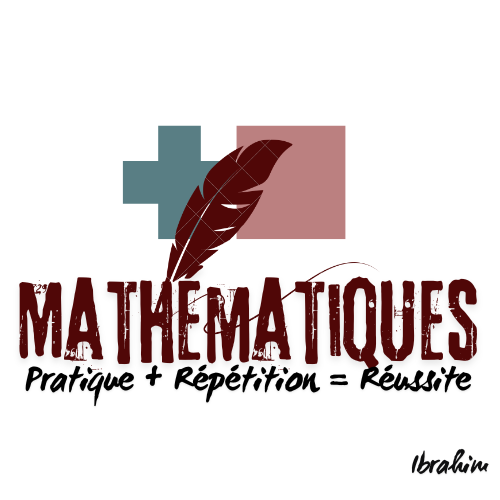
\includegraphics[width=0.5\linewidth]{LogoMath.png}
\end{figure}


\textsc{\Large 6ème Collège de Doujani }\\[1cm] % Major heading such as course name
\HRule \\[0.4cm]
{ \huge \bfseries Mathématiques Essentielles: \\ Tout pour la 6ème }\\[0.4cm]
\HRule \\[1.5cm]
\begin{center}
\begin{Large}
ATTOUMANI Ibrahim 
\end{Large}
\end{center}
    

\begin{center}
\vfill{
\includegraphics[width=0.15\linewidth]{DBS.png}}\vspace{0.5cm}\\
\begin{Large} Année 2024 - 2025
\end{Large}



\end{center}

\end{titlepage}

\pagebreak

\tableofcontents
\pagebreak

\newpage
\section{\textcolor{blue}{Introduction}}

Les mathématiques sont bien plus que des nombres et des formules : ce sont des outils puissants qui nous aident à comprendre le monde qui nous entoure, à résoudre des problèmes complexes et à développer notre capacité à penser de manière critique. Ce livre, conçu spécifiquement pour les élèves de 6ème, est une invitation à explorer ce monde fascinant des mathématiques.\\

À travers les différentes séquences de ce livre, nous allons plonger dans les principales branches des mathématiques qui seront abordées cette année. Chaque séquence a été soigneusement élaborée pour introduire progressivement les concepts mathématiques fondamentaux, tout en fournissant des exemples concrets et des exercices pour renforcer votre compréhension.\\

Nous commencerons par explorer les nombres entiers, apprendre à les manipuler et à comprendre leur place dans le système numérique. Ensuite, nous entrerons dans le monde de la géométrie, où nous découvrirons les formes, les lignes et les angles. Les opérations sur les nombres entiers seront également au programme, suivi de l'étude des distances, des cercles et des concepts de fractions.\\

Chaque séquence offre une opportunité d'apprendre de manière interactive et engageante. Nous utiliserons des outils comme la programmation pour explorer des concepts abstraits d'une manière tangible et pratique. De la proportionnalité à l'étude des angles et des formes géométriques, chaque sujet a été choisi pour enrichir votre compréhension des mathématiques et vous préparer à des défis plus complexes à l'avenir.\\

Ce livre n'est pas seulement un manuel scolaire, mais un guide pour vous aider à développer des compétences mathématiques essentielles qui vous serviront tout au long de votre parcours éducatif et au-delà. Nous espérons que vous trouverez ce voyage à travers les mathématiques aussi enrichissant que stimulant.\\

Bienvenue dans le monde captivant des mathématiques de la 6ème année!\\

\newpage

\section{\textcolor{blue}{Chapitre 1: Les Nombres Entiers}}

\subsection{\textcolor{red}{Les Entiers Naturels}}

\vspace{0.5cm}

\begin{tcolorbox}[colback=cyan!10!white, colframe=red!75!black, title=\textcolor{white}{Définition}, sharp corners=southwest]
\textcolor{black}{Les \textbf{entiers naturels} sont les nombres que nous utilisons pour compter. Ils commencent à zéro et augmentent sans fin. Ces nombres sont très importants en mathématiques et dans la vie quotidienne, car ils nous permettent de quantifier les objets et les événements.}
\end{tcolorbox}

\vspace{0.5cm}

\textcolor{purple}{Dans cette sous-section, nous allons apprendre à écrire ces nombres en toutes lettres et à les représenter graphiquement sur une demi-droite graduée.}

\vspace{0.5cm}

\begin{tcolorbox}[colback=orange!10!white, colframe=orange!75!black, title=\textcolor{white}{Exemples}, sharp corners=southwest]
\textcolor{purple}{Voici quelques exemples d'écriture en toutes lettres pour les entiers naturels :}
\begin{itemize}
    \item \textcolor{red}{0 se lit « zéro »}
    \item \textcolor{red}{1 se lit « un »}
    \item \textcolor{red}{2 se lit « deux »}
    \item \textcolor{red}{3 se lit « trois »}
    \item \textcolor{red}{4 se lit « quatre »}
    \item \textcolor{red}{5 se lit « cinq »}
    \item \textcolor{red}{6 se lit « six »}
    \item \textcolor{red}{7 se lit « sept »}
    \item \textcolor{red}{8 se lit « huit »}
    \item \textcolor{red}{9 se lit « neuf »}
\end{itemize}
\end{tcolorbox}

\vspace{0.5cm}

\textcolor{purple}{Dans un nombre, chaque chiffre occupe un certain rang détaillé dans le tableau ci-dessous:}

\vspace{0.5cm}

\begin{center}
\renewcommand{\arraystretch}{1.5}
\setlength{\arrayrulewidth}{0.5mm}

\begin{tikzpicture}
\node[rounded corners=15pt, thick, draw=gray, fill=gray!10, inner sep=10pt] (table) {
    \begin{tabular}{>{\columncolor{blue!10}}c|>{\columncolor{orange!10}}c|>{\columncolor{green!10}}c|>{\columncolor{red!10}}c}
    \hline
    \textbf{Classe des milliards} & 
    \textbf{Classe des millions} & 
    \textbf{Classe des milliers} & 
    \textbf{Unités simples} \\
    \hline
    \begin{tabular}{>{\columncolor{white}}c|>{\columncolor{white}}c|>{\columncolor{white}}c}
    \rotatebox{90}{\textcolor{black}{centaines}} &
    \rotatebox{90}{\textcolor{black}{dizaines}} &
    \rotatebox{90}{\textcolor{black}{unités}}
    \end{tabular} &
    \begin{tabular}{>{\columncolor{white}}c|>{\columncolor{white}}c|>{\columncolor{white}}c}
    \rotatebox{90}{\textcolor{black}{centaines}} &
    \rotatebox{90}{\textcolor{black}{dizaines}} &
    \rotatebox{90}{\textcolor{black}{unités}}
    \end{tabular} &
    \begin{tabular}{>{\columncolor{white}}c|>{\columncolor{white}}c|>{\columncolor{white}}c}
    \rotatebox{90}{\textcolor{black}{centaines}} &
    \rotatebox{90}{\textcolor{black}{dizaines}} &
    \rotatebox{90}{\textcolor{black}{unités}}
    \end{tabular} &
    \begin{tabular}{>{\columncolor{white}}c|>{\columncolor{white}}c|>{\columncolor{white}}c}
    \rotatebox{90}{\textcolor{black}{centaines}} &
    \rotatebox{90}{\textcolor{black}{dizaines}} &
    \rotatebox{90}{\textcolor{black}{unités}}
    \end{tabular} \\
    \hline
    \begin{tabular}{c|c|c}
    \textcolor{black}{X} &
    \textcolor{black}{X} &
    \textcolor{black}{X}
    \end{tabular} &
    \begin{tabular}{c|c|c}
    \textcolor{black}{X} &
    \textcolor{black}{X} &
    \textcolor{black}{X}
    \end{tabular} &
    \begin{tabular}{c|c|c}
    \textcolor{black}{X} &
    \textcolor{black}{X} &
    \textcolor{black}{X}
    \end{tabular} &
    \begin{tabular}{>{\columncolor{red!5}}c|>{\columncolor{red!5}}c|>{\columncolor{red!5}}c}
    \textcolor{black}{2} &
    \textcolor{black}{3} &
    \textcolor{black}{4}
    \end{tabular} \\
    \hline
    \begin{tabular}{c|c|c}
    \textcolor{black}{X} &
    \textcolor{black}{X} &
    \textcolor{black}{X}
    \end{tabular} &
    \begin{tabular}{c|c|c}
    \textcolor{black}{X} &
    \textcolor{black}{X} &
    \textcolor{black}{X}
    \end{tabular} &
    \begin{tabular}{>{\columncolor{green!5}}c|>{\columncolor{green!5}}c|>{\columncolor{green!5}}c}
    \textcolor{black}{6} &
    \textcolor{black}{5} &
    \textcolor{black}{4}
    \end{tabular} &
    \begin{tabular}{>{\columncolor{red!5}}c|>{\columncolor{red!5}}c|>{\columncolor{red!5}}c}
    \textcolor{black}{3} &
    \textcolor{black}{2} &
    \textcolor{black}{1}
    \end{tabular} \\
    \hline
    \begin{tabular}{c|c|c}
    \textcolor{black}{X} &
    \textcolor{black}{X} &
    \textcolor{black}{X}
    \end{tabular} &
    \begin{tabular}{>{\columncolor{orange!5}}c|>{\columncolor{orange!5}}c|>{\columncolor{orange!5}}c}
    \textcolor{black}{1} &
    \textcolor{black}{2} &
    \textcolor{black}{3}
    \end{tabular} &
    \begin{tabular}{>{\columncolor{green!5}}c|>{\columncolor{green!5}}c|>{\columncolor{green!5}}c}
    \textcolor{black}{9} &
    \textcolor{black}{8} &
    \textcolor{black}{7}
    \end{tabular} &
    \begin{tabular}{>{\columncolor{red!5}}c|>{\columncolor{red!5}}c|>{\columncolor{red!5}}c}
    \textcolor{black}{5} &
    \textcolor{black}{4} &
    \textcolor{black}{6}
    \end{tabular} \\
    \hline
    \begin{tabular}{c|c|c}
    \textcolor{black}{X} &
    \textcolor{black}{8} &
    \textcolor{black}{7}
    \end{tabular} &
    \begin{tabular}{>{\columncolor{orange!5}}c|>{\columncolor{orange!5}}c|>{\columncolor{orange!5}}c}
    \textcolor{black}{6} &
    \textcolor{black}{5} &
    \textcolor{black}{4}
    \end{tabular} &
    \begin{tabular}{>{\columncolor{green!5}}c|>{\columncolor{green!5}}c|>{\columncolor{green!5}}c}
    \textcolor{black}{3} &
    \textcolor{black}{2} &
    \textcolor{black}{1}
    \end{tabular} &
    \begin{tabular}{>{\columncolor{red!5}}c|>{\columncolor{red!5}}c|>{\columncolor{red!5}}c}
    \textcolor{black}{0} &
    \textcolor{black}{9} &
    \textcolor{black}{9}
    \end{tabular} \\
    \hline
    \end{tabular}
};
\end{tikzpicture}

\captionsetup{justification=centering, font=small}
\captionof{table}{\textbf{Représentation des différentes classes et unités d'un nombre.}}
\end{center}

\begin{tcolorbox}[colback=cyan!10!white, colframe=red!75!black, title=\textcolor{white}{Définition}, sharp corners=southwest]
\textcolor{black}{La demi-droite graduée est une ligne qui commence à zéro et continue indéfiniment vers la droite. Les nombres sont marqués régulièrement sur cette ligne pour représenter leur valeur. Voici une illustration de la demi-droite graduée :}

\vspace{0.5cm}

\begin{center}
\begin{tikzpicture}
    \draw[->] (0,0) -- (10,0) node[right] {\textcolor{red}{x}};
    \foreach \x in {0,1,2,3,4,5,6,7,8,9}
    \draw (\x,3pt) -- (\x,-3pt) node[below] {\textcolor{red}{\x}};
\end{tikzpicture}
\end{center}
\end{tcolorbox}

\vspace{0.5cm}

\begin{tcolorbox}[colback=cyan!10!white, colframe=lime!75!black, title=\textcolor{black}{Remarque}, sharp corners=southwest]
\textcolor{black}{Les petits traits tracés pour marquer les unités de longueur s'appellent la \textbf{\textcolor{red}{graduation}}. Lorsque l'espace entre le 0 et le 1 est trop grand, on peut utiliser une \textbf{\textcolor{red}{sous-graduation}} (en général on n'écrit pas les nombres en dessous). Au contraire, si cet espace est trop petit, on peut sauter plusieurs graduations pour ne graduer que de 5 en 5 par exemple.}
\end{tcolorbox}

\vspace{0.5cm}

\subsubsection{\textcolor{green}{Comparer, Ranger, Encadrer ou Intercaler des Entiers Naturels}}

\textcolor{purple}{Dans cette partie, nous allons apprendre à comparer, ranger, encadrer et intercaler des entiers naturels. Ces compétences sont utiles pour organiser et manipuler les nombres efficacement.}

\vspace{0.5cm}

\textcolor{purple}{**Comparer** des entiers naturels consiste à déterminer lequel est plus grand ou plus petit. Les signes utilisés pour comparer sont \(<\) (strictement inférieur à), \(>\) (strictement supérieur à), \(\leq\) (inférieur ou égal à), et \(\geq\) (supérieur ou égal à).}

\vspace{0.5cm}

\begin{tcolorbox}[colback=orange!10!white, colframe=orange!75!black, title=\textcolor{white}{Exemples}, sharp corners=southwest]

\begin{itemize}
    \item \textcolor{red}{\(3 < 5\) (trois est strictement inférieur à cinq)}
    \item \textcolor{red}{\(7 > 4\) (sept est strictement supérieur à quatre)}
    \item \textcolor{red}{\(6 \leq 6\) (six est inférieur ou égal à six)}
    \item \textcolor{red}{\(9 \geq 2\) (neuf est supérieur ou égal à deux)}
\end{itemize}.
\end{tcolorbox}

\vspace{0.5cm}

\textcolor{purple}{**Ranger** des entiers naturels signifie les organiser dans l'ordre croissant (du plus petit au plus grand) ou décroissant (du plus grand au plus petit).}

\vspace{0.5cm}

Considérons les nombres suivants en ordre croissant :

\[ 1 < 2 < 3 < 4 < 5 < 6 \]

Pour mieux visualiser l'ordre croissant, regardons la représentation graphique ci-dessous :

\begin{center}
\begin{tikzpicture}[scale=1.5]
  \draw[->] (0,0) -- (7,0) node[anchor=north west] {Nombres};
  \foreach \x in {1, 2, 3, 4, 5, 6}
    \draw (\x,0) -- (\x,0.2) node[above] {\x};
  
  \draw[thick, -{Latex[length=3mm, width=2mm]}] (0.5,0.5) -- (6.5,0.5);
  \node at (3.5, 0.75) {Ordre croissant};
\end{tikzpicture}
\end{center}

\begin{figure}[H]
    \centering
    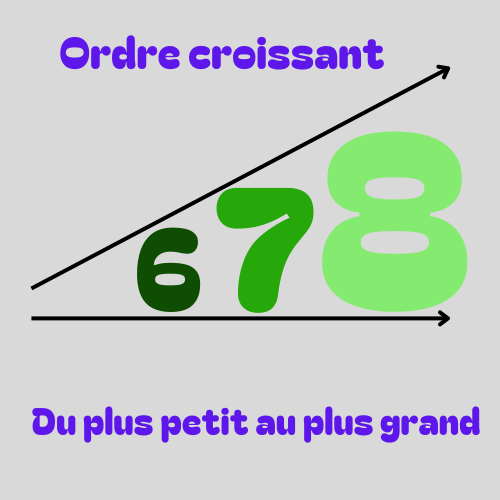
\includegraphics[width=0.49\linewidth]{ordreCroissant.png}
    \caption{Progression en Ordre Croissant}
    \label{fig:enter-label}
\end{figure}

Considérons les nombres suivants en ordre décroissant :

\[ 6 > 5 > 4 > 3 > 2 > 1 \]

Pour mieux visualiser l'ordre décroissant, regardons la représentation graphique ci-dessous :

\begin{center}
\begin{tikzpicture}[scale=1.5]
  \draw[->] (0,0) -- (7,0) node[anchor=north west] {Nombres};
  \foreach \x in {1, 2, 3, 4, 5, 6}
    \draw (\x,0) -- (\x,0.2) node[above] {\x};
  
  \draw[thick, -{Latex[length=3mm, width=2mm]}] (6.5,0.5) -- (0.5,0.5);
  \node at (3.5, 0.75) {Ordre décroissant};
\end{tikzpicture}
\end{center}

\begin{figure}[H]
    \centering
    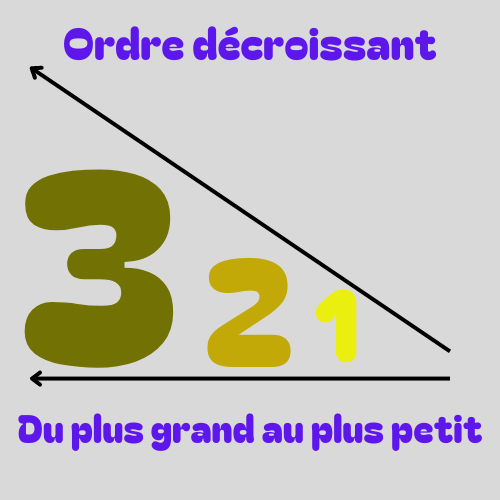
\includegraphics[width=0.49\linewidth]{ordreDecroissante.png}
    \caption{Progression en Ordre Décroissante}
    \label{fig:enter-label}
\end{figure}

\textcolor{purple}{**Encadrer** un nombre consiste à trouver deux nombres entre lesquels il se trouve. Cela peut aider à estimer la position d'un nombre par rapport aux autres.}

\vspace{0.25cm}

\begin{tcolorbox}[colback=orange!10!white, colframe=orange!75!black, title=\textcolor{white}{Exemples}, sharp corners=southwest]

\begin{itemize}
    \item \textcolor{red}{\(4 < 6 < 8\) (six est encadré entre quatre et huit)}
\end{itemize}.
\end{tcolorbox}

Considérons l'encadrement du nombre \(x = 3\) tel que \(a = 1 \leq x \leq b = 5\).

\[
a \leq x \leq b
\]

Pour mieux visualiser l'encadrement d'un nombre, regardons la représentation graphique ci-dessous :

\begin{center}
\begin{tikzpicture}[scale=1.5]
  \draw[->] (0,0) -- (7,0) node[anchor=north west] {Nombres};
  \foreach \x in {0, 1, 2, 3, 4, 5, 6}
    \draw (\x,0) -- (\x,0.2) node[above] {\x};
  
  \draw[thick, -{Latex[length=3mm, width=2mm]}] (1.2,0.5) -- (4.8,0.5);
  \node at (3, 0.75) {\(a \leq x \leq b\)};
  
  \draw[dashed] (1,0) -- (1,0.5);
  \node[below] at (1,0) {\(a\)};
  
  \draw[dashed] (5,0) -- (5,0.5);
  \node[below] at (5,0) {\(b\)};
  
  \node at (3, 0.25) {\(x\)};
\end{tikzpicture}
\end{center}

\textcolor{purple}{**Intercaler** un nombre signifie le placer correctement entre deux autres nombres. Cela aide à mieux comprendre la position relative des nombres.}

\vspace{0.4cm}

\begin{tcolorbox}[colback=orange!10!white, colframe=orange!75!black, title=\textcolor{white}{Exemples}, sharp corners=southwest]

\begin{itemize}
    \item \textcolor{red}{y = 3 est entre x = 2 et z = 4}
\end{itemize}.
\end{tcolorbox}

Pour mieux visualiser l'intercalation d'un nombre, regardons la représentation graphique ci-dessous :

\begin{center}
\begin{tikzpicture}[scale=1.5]
  \draw[->] (0,0) -- (7,0) node[anchor=north west] {Nombres};
  \foreach \x in {1, 2, 3, 4, 5, 6}
    \draw (\x,0) -- (\x,0.2) node[above] {\x};
  
  \draw[thick, -{Latex[length=3mm, width=2mm]}] (1,0.5) -- (5,0.5);
  \node at (3, 0.75) {\( x < y < z \)};
  
  \draw[dashed] (2,0) -- (2,0.5);
  \node[below] at (2,0) {\(x\)};
  
  \draw[dashed] (4,0) -- (4,0.5);
  \node[below] at (4,0) {\(z\)};
  
  \draw[fill=black] (3,0) circle (1.5pt);
  \node[below] at (3,0) {\(y\)};
  
\end{tikzpicture}
\end{center}

\vspace{0.5cm}

\begin{tcolorbox}[colback=orange!10!white, colframe=yellow!80!black, title=\textcolor{white}{Application directe}, 
                  sharp corners=south]
    \textbf{Exercice 1 :} Trouvez les nombres entiers naturels entre 10 et 20.

    \vspace{0.2cm}

    \textbf{Exercice 2 :} Écrivez les nombres suivants en toutes lettres : 13, 25, 37, 48, 59.

    \vspace{0.2cm}

    \textbf{Exercice 3 :} Représentez graphiquement les nombres 0, 1, 2, 3, 4, et 5 sur une demi-droite graduée.

    \vspace{0.2cm}

    \textbf{Exercice 4 :} Comparez les entiers naturels suivants en utilisant les signes \(<\), \(>\), \(\leq\), ou \(\geq\) : 7 et 9, 12 et 12, 15 et 8.

    \vspace{0.2cm}

    \textbf{Exercice 5 :} Rangez les nombres suivants dans l'ordre décroissant : 45, 23, 89, 12, 67.

    \vspace{0.2cm}

    \textbf{Exercice 6 :} Encadrez le nombre 6 entre deux entiers naturels.

    \vspace{0.2cm}

    \textbf{Exercice 7 :} Intercalez le nombre 5 entre les nombres 3 et 7.
\end{tcolorbox}

\begin{tcolorbox}[colback=cyan!10!white, colframe=cyan!75!black, title=\textcolor{white}{Récapitulatif}, 
                  sharp corners=south]
    \textcolor{black}{Dans cette section, nous avons exploré les concepts fondamentaux liés aux \textbf{nombres entiers naturels}. Voici les points essentiels à retenir :}

    \begin{itemize}
        \item \textbf{Les entiers naturels} sont les nombres que nous utilisons pour compter, comme 0, 1, 2, 3, etc.
        \item Chaque chiffre dans un nombre occupe un \textbf{rang} spécifique (unités, dizaines, centaines, etc.).
        \item La \textbf{demi-droite graduée} est utilisée pour représenter les entiers naturels graphiquement.
        \item Les \textbf{opérations de comparaison} permettent de déterminer si un nombre est plus grand, plus petit, ou égal à un autre.
        \item \textbf{Ranger} des entiers naturels signifie les organiser dans un ordre croissant ou décroissant.
        \item \textbf{Encadrer} un nombre consiste à trouver deux nombres entre lesquels il se situe.
        \item \textbf{Intercaler} un nombre consiste à le placer correctement entre deux autres nombres.
    \end{itemize}

    \textcolor{black}{Ces concepts sont cruciaux pour comprendre et manipuler les nombres dans les mathématiques de base.}
\end{tcolorbox}


\vspace{0.5cm}

\subsection{\textcolor{red}{Les Entiers Relatifs}}

\vspace{0.35cm}

\begin{tcolorbox}[colback=cyan!10!white, colframe=red!75!black, title=\textcolor{white}{Définition}, 
                  sharp corners=southwest]

\textcolor{black}{Les entiers relatifs incluent les entiers naturels ainsi que leurs opposés négatifs. Ces nombres permettent de représenter des quantités en dessous de zéro, comme les températures négatives ou les dettes.}
\end{tcolorbox}

\textcolor{purple}{Dans cette sous-section, nous apprendrons à écrire ces nombres en toutes lettres et à les représenter sur une demi-droite graduée.}

\vspace{0.4cm}

\begin{tcolorbox}[colback=orange!10!white, colframe=orange!75!black, title=\textcolor{white}{Exemples}, sharp corners=southwest]
\textcolor{purple}{Voici quelques exemples d'écriture en toutes lettres pour les entiers relatifs :}

\begin{itemize}
    \item \textcolor{red}{-3 se lit « moins trois »}
    \item \textcolor{red}{-2 se lit « moins deux »}
    \item \textcolor{red}{-1 se lit « moins un »}
    \item \textcolor{red}{0 se lit « zéro »}
    \item \textcolor{red}{1 se lit « un »}
    \item \textcolor{red}{2 se lit « deux »}
    \item \textcolor{red}{3 se lit « trois »}
\end{itemize}.
\end{tcolorbox}

\begin{tcolorbox}[colback=cyan!10!white, colframe=lime!75!black, title=\textcolor{black}{Remarque}, 
                  sharp corners=southwest]
\textcolor{black}{Sur une demi-droite graduée, les nombres négatifs sont placés à gauche de zéro, et les nombres positifs à droite. Voici une illustration :}

\begin{center}
\begin{tikzpicture}
    \draw[->] (-4,0) -- (4,0) node[right] {\textcolor{red}{x}};
    \foreach \x in {-3,-2,-1,0,1,2,3}
    \draw (\x,3pt) -- (\x,-3pt) node[below] {\textcolor{red}{\x}};
\end{tikzpicture}
\end{center}

\end{tcolorbox}

\vspace{0.5cm}

\textcolor{purple}{Imaginons que vous n'avez rien, soit 0 pièce (pas d'argent). Puis, vous faites un emprunt de 3 pièces à votre ami. Vous passez donc de 0 à -3, car vous devez maintenant 3 pièces à votre ami (c'est une dette). Ensuite, votre père vous donne 10 pièces comme argent de poche. Cela vous fait passer de -3 à 7 pièces, car dans les 10 pièces que vous avez reçues, vous en retirez 3 pour rembourser la dette envers votre ami. Voici comment cela se présente :}

\vspace{0.5cm}

\begin{center}
\begin{tikzpicture}
    \draw[->] (-5,0) -- (10,0) node[right] {\textcolor{red}{x}};
    \foreach \x in {-4,-3,-2,-1,0,1,2,3,4,5,6,7,8,9}
    \draw (\x,3pt) -- (\x,-3pt) node[below] {\textcolor{red}{\x}};
    
    \draw[fill=blue] (0,0) circle (2pt) node[above] {0};
    \draw[fill=blue] (-3,0) circle (2pt) node[above] {-3};
    \draw[fill=blue] (7,0) circle (2pt) node[above] {7};
    
    \node[align=center, above] at (0, 1) {\textcolor{blue}{Départ : 0}};
    \node[align=center, above] at (-3, 1) {\textcolor{blue}{Emprunt : -3}};
    \node[align=center, above] at (7, 1) {\textcolor{blue}{Après remboursement : 7}};
\end{tikzpicture}
\end{center}

\subsubsection{\textcolor{green}{Comparer, Ranger, Encadrer ou Intercaler des Entiers Relatifs}}

\textcolor{purple}{Comparer, ranger, encadrer et intercaler des entiers relatifs sont des compétences essentielles pour comprendre et manipuler ces nombres. Ces opérations nous aident à organiser les nombres négatifs et positifs et à les utiliser dans des situations variées.}

\vspace{0.35cm}

\textcolor{purple}{**Comparer** des entiers relatifs se fait avec les mêmes signes que pour les entiers naturels : \(<\), \(>\), \(\leq\), et \(\geq\).}

\vspace{0.5cm}

\begin{tcolorbox}[colback=orange!10!white, colframe=orange!75!black, title=\textcolor{white}{Exemples}, sharp corners=southwest]
\begin{itemize}
    \item \textcolor{red}{-3 < -1 (moins trois est strictement inférieur à moins un)}
    \item \textcolor{red}{2 > -4 (deux est strictement supérieur à moins quatre)}
    \item \textcolor{red}{$-2 \leq 0$ (moins deux est inférieur ou égal à zéro)}
    \item \textcolor{red}{$3 \geq -1$ (trois est supérieur ou égal à moins un)}
\end{itemize}.
\end{tcolorbox}

\textcolor{purple}{**Ranger** des entiers relatifs consiste à les organiser dans l'ordre croissant ou décroissant, en tenant compte des nombres négatifs et positifs.}

\vspace{0.35cm}

\textcolor{purple}{**Encadrer** un nombre relatif consiste à trouver deux entiers relatifs entre lesquels il se trouve. Cela peut être utile pour estimer sa position.}

\vspace{0.4cm}

\begin{tcolorbox}[colback=orange!10!white, colframe=orange!75!black, title=\textcolor{white}{Exemples}, sharp corners=southwest]

\begin{itemize}
    \item \textcolor{red}{-2 < 0 < 3 (zéro est encadré entre moins deux et trois)}
\end{itemize}.
\end{tcolorbox}

\textcolor{purple}{**Intercaler** un nombre relatif signifie le placer entre deux autres nombres. Cela aide à comprendre sa position relative dans l'ensemble des entiers.}

\vspace{0.4cm}

\begin{tcolorbox}[colback=orange!10!white, colframe=orange!75!black, title=\textcolor{white}{Exemples}, sharp corners=southwest]

\begin{itemize}
    \item \textcolor{red}{1 est entre 0 et 2}
    \item \textcolor{red}{-15 est entre -16 et -14}
\end{itemize}
\end{tcolorbox}

\begin{tcolorbox}[colback=yellow!10!white, colframe=yellow!80!black, title=\textcolor{white}{Application directe}, sharp corners=southwest]

\textcolor{purple}{
Écris les entiers relatifs suivants en toutes lettres :
}
\begin{itemize}
    \item $-4$
    \item $7$
    \item $-12$
    \item $0$
    \item $-9$
\end{itemize}

\vspace{0.4cm}

\textcolor{purple}{
Tracez une demi-droite graduée, puis placez-y les entiers relatifs suivants : $-3$, $-1$, $2$, $4$, $-2$.
}


\end{tcolorbox}

\vspace{0.5cm}

\begin{tcolorbox}[colback=yellow!10!white, colframe=cyan!80!black, title=\textcolor{black}{Récapitulatif}, sharp corners=southwest]
\textcolor{purple}{Dans cette leçon, nous avons appris à écrire et à représenter les entiers relatifs. N'oubliez pas que les nombres négatifs sont simplement des entiers avec un signe moins devant, et ils se trouvent à gauche de zéro sur une droite graduée.}
\end{tcolorbox}

\subsection{\textcolor{red}{Opérations sur les Nombres Entiers}}

\subsubsection{\textcolor{green}{Additions et Soustractions}}

\vspace{0.5cm}

\begin{tcolorbox}[colback=cyan!10!white, colframe=red!75!black, title=\textcolor{white}{Définition}, 
                  sharp corners=southwest]
                  
\textcolor{purple}{Les additions et soustractions sont les opérations de base pour combiner ou comparer des nombres. Nous allons explorer comment effectuer ces opérations avec des entiers.}
\end{tcolorbox}

\vspace{0.5cm}

\textcolor{purple}{**Additionner** des nombres signifie les combiner (les ajoutés entre eux) pour obtenir un total.}

\vspace{0.15cm}

\textbf{Exemples :}

\begin{itemize}
    \item \textcolor{red}{\(3 + 5 = 8\)}
\end{itemize}

\begin{figure}[H]
\centering
\begin{tikzpicture}
    % Capsule orange clair
    \fill[orange!20] (-0.5, -0.5) rectangle (10, 1.5);

    % Rectangles pour le nombre 3
    \fill[blue!70] (0.2, 0) rectangle (1.2, 1);
    \fill[blue!70] (1.3, 0) rectangle (2.3, 1);
    \fill[blue!70] (2.4, 0) rectangle (3.4, 1);

    % Espacement
    \draw[dashed] (3.5, 0) -- (3.5, 1);

    % Rectangles pour le nombre 5
    \fill[green!70] (4.0, 0) rectangle (5.0, 1);
    \fill[green!70] (5.1, 0) rectangle (6.1, 1);
    \fill[green!70] (6.2, 0) rectangle (7.2, 1);
    \fill[green!70] (7.3, 0) rectangle (8.3, 1);
    \fill[green!70] (8.4, 0) rectangle (9.4, 1);

    % Label du total
    \node at (4.5, 1.2) {\footnotesize \textbf{Total}};
    
    % Résultat
    \node at (4.5, -0.5) {\textcolor{red}{8}};
\end{tikzpicture}
\caption{Illustration de \(3 + 5\) avec des rectangles}
\end{figure}

\begin{itemize}
    \item \textcolor{red}{\(-3 + 4 = 1\)}
\end{itemize}

\begin{figure}[H]
\centering
\begin{tikzpicture}
    % Capsule orange clair
    \fill[orange!20] (-0.5, -0.5) rectangle (9, 1.5);

    % Rectangles pour le nombre -3 (négatifs en rouge)
    \fill[red!70] (0.2, 0) rectangle (1.2, 1);
    \fill[red!70] (1.3, 0) rectangle (2.3, 1);
    \fill[red!70] (2.4, 0) rectangle (3.4, 1);

    % Espacement
    \draw[dashed] (3.5, 0) -- (3.5, 1);

    % Rectangles pour le nombre 4
    \fill[cyan!70] (4.0, 0) rectangle (5.0, 1);
    \fill[cyan!70] (5.1, 0) rectangle (6.1, 1);
    \fill[cyan!70] (6.2, 0) rectangle (7.2, 1);
    \fill[cyan!70] (7.3, 0) rectangle (8.3, 1);

    % Label du total
    \node at (4.5, 1.2) {\footnotesize \textbf{Total}};
    
    % Résultat
    \node at (4.5, -0.5) {\textcolor{red}{1}};
\end{tikzpicture}
\caption{Illustration de \(-3 + 4\) avec des rectangles}
\end{figure}

\vspace{0.5cm}

\textcolor{purple}{**Soustraire** un nombre signifie enlever une quantité d'un autre nombre.}

\vspace{0.15cm}

\textbf{Exemples :}

\begin{itemize}
    \item \textcolor{red}{\(7 - 2 = 5\)}
\end{itemize}

\begin{figure}[h]
\centering
\begin{tikzpicture}
    % Capsule orange clair
    \fill[orange!20] (-0.5, -0.5) rectangle (16.5, 1.5);

    % Rectangles pour le nombre 7
    \fill[blue!70] (0.2, 0) rectangle (1.2, 1);
    \fill[blue!70] (1.3, 0) rectangle (2.3, 1);
    \fill[blue!70] (2.4, 0) rectangle (3.4, 1);
    \fill[blue!70] (3.5, 0) rectangle (4.5, 1);
    \fill[blue!70] (4.6, 0) rectangle (5.6, 1);
    \fill[blue!70] (5.7, 0) rectangle (6.7, 1);
    \fill[blue!70] (6.8, 0) rectangle (7.8, 1);

    % Espacement
    \draw[dashed] (7.9, 0) -- (7.9, 1);

    % Rectangles pour le nombre 2
    \fill[red!70] (8.0, 0) rectangle (9.0, 1);
    \fill[red!70] (9.1, 0) rectangle (10.1, 1);

    % Résultat (5)
    \fill[green!70] (10.5, 0) rectangle (11.5, 1);
    \fill[green!70] (11.6, 0) rectangle (12.6, 1);
    \fill[green!70] (12.7, 0) rectangle (13.7, 1);
    \fill[green!70] (13.8, 0) rectangle (14.8, 1);
    \fill[green!70] (14.9, 0) rectangle (15.9, 1);

    % Label du total
    \node at (10.5, 1.2) {\footnotesize \textbf{Résultat}};
    
    % Résultat
    \node at (12, -0.5) {\textcolor{red}{5}};
\end{tikzpicture}
\caption{Illustration de \(7 - 2\) avec des rectangles}
\end{figure}

\vspace{0.4cm}

\begin{itemize}
    \item \textcolor{red}{\(-5 - 2 = -7\)}
\end{itemize}

\begin{figure}[H]
\centering
\begin{tikzpicture}
    % Capsule orange clair
    \fill[orange!20] (-0.5, -0.5) rectangle (16.5, 1.5);

    % Rectangles pour le nombre -5 (négatifs en rouge)
    \fill[red!70] (0.2, 0) rectangle (1.2, 1);
    \fill[red!70] (1.3, 0) rectangle (2.3, 1);
    \fill[red!70] (2.4, 0) rectangle (3.4, 1);
    \fill[red!70] (3.5, 0) rectangle (4.5, 1);
    \fill[red!70] (4.6, 0) rectangle (5.6, 1);

    % Espacement
    \draw[dashed] (5.7, 0) -- (5.7, 1);

    % Rectangles pour le nombre -2
    \fill[cyan!70] (6.0, 0) rectangle (7.0, 1);
    \fill[cyan!70] (7.1, 0) rectangle (8.1, 1);

    % Résultat (-7)
    \fill[green!70] (8.5, 0) rectangle (9.5, 1);
    \fill[green!70] (9.6, 0) rectangle (10.6, 1);
    \fill[green!70] (10.7, 0) rectangle (11.7, 1);
    \fill[green!70] (11.8, 0) rectangle (12.8, 1);
    \fill[green!70] (12.9, 0) rectangle (13.9, 1);
    \fill[green!70] (14.0, 0) rectangle (15.0, 1);
    \fill[green!70] (15.1, 0) rectangle (16.1, 1);

    % Label du total
    \node at (8.5, 1.2) {\footnotesize \textbf{Résultat}};
    
    % Résultat
    \node at (11, -0.5) {\textcolor{red}{-7}};
\end{tikzpicture}
\caption{Illustration de \(-5 - 2\) avec des rectangles}
\end{figure}

\vspace{0.3cm}

\subsubsection{\textcolor{green}{Multiplications}}

\begin{tcolorbox}[colback=cyan!10!white, colframe=red!75!black, title=\textcolor{white}{Définition}, 
                  sharp corners=southwest]

\textcolor{purple}{La multiplication est une opération qui consiste à ajouter un nombre à lui-même un certain nombre de fois. Nous allons voir comment multiplier des entiers.}
\end{tcolorbox}

\vspace{0.3cm}

\textcolor{purple}{Relation de signes : Lorsque l'on multiplie ou divise des nombres, la règle est la suivante :}
\begin{itemize}
    \item \textcolor{purple}{Le produit ou le quotient de deux nombres de même signe (positif avec positif ou négatif avec négatif) est \textbf{positif}.}
    \item \textcolor{purple}{Le produit ou le quotient de deux nombres de signes opposés (positif avec négatif) est \textbf{négatif}.}
\end{itemize}

\vspace{0.2cm}

\begin{tcolorbox}[colback=lightblue, colframe=navyblue, title=\textcolor{white}{Relations de Signes}, sharp corners=southwest]
\centering
\begin{tabular}{|c|c|c|}
\hline
\textbf{Opération} & \textbf{Résultat} & \textbf{Couleur} \\
\hline
\cellcolor{lightgray} \(- \, (+) = -\) & \textcolor{red}{Négatif} & \textcolor{red}{\(-\)} \\
\hline
\cellcolor{lightblue} \(+ \, (+) = +\) & \textcolor{purple}{Positif} & \textcolor{purple}{\(+\)} \\
\hline
\cellcolor{lightgray} \(- \, (-) = +\) & \textcolor{purple}{Positif} & \textcolor{purple}{\(+\)} \\
\hline
\cellcolor{lightblue} \(+ \, (-) = -\) & \textcolor{red}{Négatif} & \textcolor{red}{\(-\)} \\
\hline
\end{tabular}
\end{tcolorbox}

\vspace{0.3cm}

\begin{tcolorbox}[colback=cyan!10!white, colframe=orange!75!black, title=\textcolor{white}{Exemples}, sharp corners=southwest]
\centering
\begin{minipage}{0.45\textwidth}
\centering
\textcolor{blue}{Multiplication de 10 avec 5} \\
\opmul[voperator=bottom, displayshiftintermediary=none]{10}{5}
\end{minipage}%
\hfill
\begin{minipage}{0.45\textwidth}
\centering
\textcolor{blue}{Multiplication de 12 avec 11} \\
\opmul[voperator=bottom, displayshiftintermediary=none]{12}{11}
\end{minipage}
\end{tcolorbox}

\begin{tcolorbox}[colback=orange!10!white, colframe=orange!75!black, sharp corners=south, boxrule=0.8mm, title=Explication des Exemples]
    \textbf{Multiplication de 10 par 5 :}
    \[
    \opmul[voperator=bottom, displayshiftintermediary=none]{10}{5}
    \]
    \textcolor{red}{(La multiplication de 10 par 5 est directe : 10 multiplié par 5 donne 50.)}
    
    \textbf{Explication :} Nous multiplions 10 par 5. Comme 10 est un nombre entier, nous multiplions simplement les chiffres 10 et 5. Le résultat est 50.

    \textbf{Multiplication de 12 par 11 :}
    \[
    \opmul[voperator=bottom, displayshiftintermediary=none]{12}{11}
    \]
    \textcolor{red}{(Pour multiplier 12 par 11, nous utilisons la méthode distributive : (10 + 2) × (10 + 1). On obtient 120 + 12 = 132.)}
    
    \textbf{Explication :} Nous multiplions 12 par 11 en utilisant la méthode distributive : 
    \begin{itemize}
        \item Décomposez 11 en 10 + 1.
        \item Multipliez 12 par 10 pour obtenir 120.
        \item Multipliez 12 par 1 pour obtenir 12.
        \item Additionnez les deux résultats : 120 + 12 = 132.
    \end{itemize}
\end{tcolorbox}

\vspace{0.4cm}

\textcolor{purple}{**Déroulement des Multiplications :**}

\begin{enumerate}
    \item \textcolor{purple}{Pour \(10 \times 5\) :}
    \begin{enumerate}
        \item \textcolor{purple}{On peut visualiser cela comme ajouter 10 cinq fois :}
        \[
        10 + 10 + 10 + 10 + 10 = 50
        \]
    \end{enumerate}

    \item \textcolor{purple}{Pour \(12 \times 11\) :}
    \begin{enumerate}
        \item \textcolor{purple}{On peut visualiser cela comme ajouter 12 onze fois :}
        \[
        12 + 12 + 12 + 12 + 12 + 12 + 12 + 12 + 12 + 12 + 12 = 132
        \]
    \end{enumerate}
\end{enumerate}


\begin{tcolorbox}[colback=cyan!10!white, colframe=red!75!black, title=\textcolor{white}{Définition},
                  sharp corners=southwest]
                  
\textcolor{black}{ Un multiple d'un nombre est le produit de ce nombre par un autre nombre entier. Par exemple, 24 est un multiple de 4 (car \(4 \times 6 = 24\)).}
\end{tcolorbox}

\subsubsection{\textcolor{green}{Division Euclidienne}}

\vspace{0.5cm}

\begin{tcolorbox}[colback=cyan!10!white, colframe=red!75!black, title=\textcolor{white}{Définition}, 
                  sharp corners=southwest]

\textcolor{black}{La division euclidienne consiste à diviser un nombre, appelé \textcolor{red}{dividende}, par un autre nombre, appelé \textcolor{red}{diviseur}, pour obtenir un \textcolor{red}{quotient} et un \textcolor{red}{reste}. Cette division est utile pour déterminer combien de fois un nombre peut être réparti en parts égales, et ce qui reste.}
\end{tcolorbox}

\vspace{0.5cm}

\textcolor{purple}{Voici les termes importants :}
\begin{itemize}
    \item \textcolor{red}{Dividende : Le nombre que l'on souhaite diviser.}
    \item \textcolor{red}{Diviseur : Le nombre par lequel on divise.}
    \item \textcolor{red}{Quotient : Le résultat entier de la division.}
    \item \textcolor{red}{Reste : Ce qui reste après la division.}
\end{itemize}


\begin{figure}[H]
    \centering
    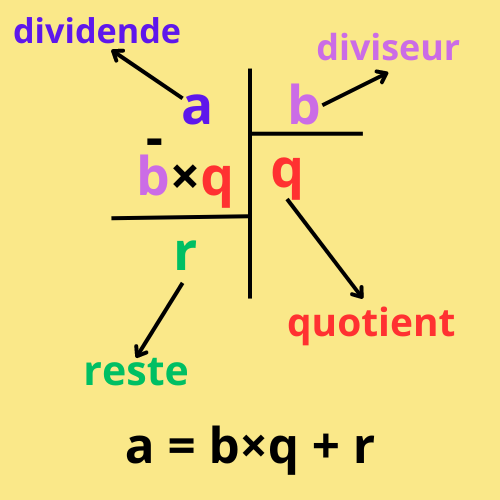
\includegraphics[width=0.55 \linewidth]{division_euclidienne.png}
    \caption{Illustration de la Division Euclidienne}
    \label{fig:enter-label}
\end{figure}

\vspace{0.1cm}

\textcolor{purple}{Exemple }

\begin{tcolorbox}[colback=cyan!10!white, colframe=orange!75!black, title=\textcolor{white}{Division Euclidienne de 27 par 4 avec reste non nul}, sharp corners=southwest]
\centering
\opidiv[displayintermediary=all,voperation=top]{27}{4}
\end{tcolorbox}

\textcolor{purple}{\textbf{Explication du déroulement :}}

\begin{enumerate}
    \item \textcolor{purple}{\textbf{Division :} Nous commençons par diviser 27 par 4. On cherche combien de fois 4 peut entrer dans 27 sans dépasser ce nombre. La réponse est 6 fois, car \(4 \times 6 = 24\).}
    \item \textcolor{purple}{\textbf{Soustraction :} Ensuite, on soustrait 24 de 27. Cette soustraction donne un reste de 3, car \(27 - 24 = 3\).}
    \item \textcolor{purple}{\textbf{Résultat :} La division euclidienne nous donne donc un quotient de 6 et un reste de 3. En d'autres termes, 27 divisé par 4 donne 6 avec un reste de 3.}
\end{enumerate}

\vspace{0.1cm}

\textcolor{purple}{Ainsi, la division euclidienne de 27 par 4 s'écrit : 
\[ 27 = 4 \times 6 + 3 \]}

\textcolor{purple}{Cette méthode nous permet de comprendre comment un nombre peut être divisé en parties égales et combien il en reste après avoir divisé complètement.}


\vspace{0.4cm}

\begin{tcolorbox}[colback=cyan!10!white, colframe=orange!75!black, title=\textcolor{white}{Division Euclidienne de 27 par 4 avec reste zéro}, 
                  sharp corners=southwest]
\centering
\opidiv[displayintermediary=all,voperation=top]{27}{3}
\end{tcolorbox}

\vspace{0.4cm}

\textcolor{purple}{\textbf{Explication du déroulement :}}

\begin{enumerate}
    \item \textcolor{purple}{\textbf{Division :} Nous commençons par diviser 27 par 3. On cherche combien de fois 3 peut entrer dans 27 sans dépasser ce nombre. La réponse est 9 fois, car \(3 \times 9 = 27\).}
    \item \textcolor{purple}{\textbf{Soustraction :} Ensuite, on soustrait 27 de 27. Cette soustraction donne un reste de 0, car \(27 - 27 = 0\).}
    \item \textcolor{purple}{\textbf{Résultat :} La division euclidienne nous donne donc un quotient de 9 et un reste de 0. En d'autres termes, 27 divisé par 3 donne 9 sans reste.}
\end{enumerate}

\textcolor{purple}{Ainsi, la division euclidienne de 27 par 3 s'écrit : 
\[ 27 = 3 \times 9 + 0 \]}

\textcolor{purple}{Cette méthode nous montre que 27 peut être divisé en parties égales de 3 sans qu'il reste de quantité. Cela signifie que 3 est un diviseur exact de 27.}

\vspace{0.15cm}

\begin{tcolorbox}[colback=cyan!10!white, colframe=pink!75!black, title=\textcolor{white}{Les types de divisions}, sharp corners=southwest]
En mathématiques, il existe principalement deux types de divisions lorsque l'on travaille avec des nombres entiers.

\vspace{0.2cm}

1. \textbf{Division avec reste non nul} : Lorsque l'on divise un nombre entier (appelé \textbf{dividende}) par un autre nombre entier (appelé \textbf{diviseur}), il se peut que le diviseur ne se divise pas exactement dans le dividende. Dans ce cas, après avoir trouvé combien de fois le diviseur peut entrer dans le dividende (c'est le \textbf{quotient}), il reste une certaine quantité, appelée le \textbf{reste}. Par exemple, si l'on divise 27 par 4, on obtient un quotient de 6 et un reste de 3, car \(27 = 4 \times 6 + 3\).

\vspace{0.2cm}

2. \textbf{Division avec reste zéro} : Dans ce type de division, le diviseur se divise exactement dans le dividende, c'est-à-dire qu'il n'y a pas de reste. Le quotient est donc le nombre entier de fois que le diviseur peut être multiplié pour atteindre le dividende. Par exemple, si l'on divise 24 par 6, on obtient un quotient de 4 et un reste de 0, car \(24 = 6 \times 4\). Cela signifie que 6 est un diviseur exact de 24, et que 24 est un multiple de 6.

\vspace{0.2cm}

Ces deux types de divisions sont importants pour comprendre comment les nombres peuvent être décomposés et regroupés. Dans le cas où le reste est zéro, cela indique une relation particulière entre le dividende et le diviseur, où le diviseur est un facteur exact du dividende.
\end{tcolorbox}

\vspace{0.15cm}

\begin{tcolorbox}[colback=cyan!10!white, colframe=lime!75!black, title=\textcolor{black}{Remarque}, 
                  sharp corners=southwest]
\textcolor{black}{
Il est possible de mélanger les opérations d'addition, de soustraction, de multiplication, et de division dans une même expression. Cependant, certaines opérations ont des priorités sur d'autres. Par exemple, les multiplications et les divisions doivent être effectuées avant les additions et les soustractions. Nous verrons plus en détail ces priorités opératoires par la suite.
}
\end{tcolorbox}

\subsubsection{\textcolor{green}{Priorités Opératoires}}

\vspace{0.25cm}

\begin{tcolorbox}[colback=cyan!10!white, colframe=red!75!black, title=\textcolor{white}{Définition}, 
                  sharp corners=southwest]

\textcolor{black}{Les priorités opératoires déterminent l'ordre dans lequel les opérations doivent être effectuées dans une expression mathématique pour obtenir le bon résultat.}
\end{tcolorbox}

\vspace{0.35cm}

\textcolor{purple}{Lors de la résolution d'expressions arithmétiques, il est important de suivre un ordre précis pour effectuer les opérations correctement. Voici les priorités opératoires à respecter :}

\vspace{0.35cm}

\begin{enumerate}
    \item \textcolor{red}{**Parenthèses** : Les opérations à l'intérieur des parenthèses doivent être effectuées en premier. Cela permet de regrouper les calculs et d'assurer leur exécution dans le bon ordre.}
    \item \textcolor{red}{**Multiplications et Divisions** : Ensuite, on effectue les multiplications et les divisions de gauche à droite. Ces opérations ont la même priorité, donc on les traite dans l'ordre où elles apparaissent.}
    \item \textcolor{red}{**Additions et Soustractions** : Enfin, on réalise les additions et les soustractions de gauche à droite. Comme pour les multiplications et divisions, ces opérations ont la même priorité.}
\end{enumerate}

\vspace{0.25cm}

\textcolor{purple}{Voici un exemple simple pour illustrer ces règles :}

\begin{itemize}
    \item \textcolor{purple}{Considérons l'expression : \( 4 + 3 \times 2 \).}
    \begin{itemize}
        \item \textcolor{red}{Il n'y a pas de parenthèses, donc on passe directement aux multiplications et divisions.}
        \item \textcolor{red}{Nous devons effectuer la multiplication avant l'addition. Calculons donc \( 3 \times 2 = 6 \).}
        \item \textcolor{red}{Ensuite, on effectue l'addition : \( 4 + 6 = 10 \).}
    \end{itemize}

    \item \textcolor{purple}{Un autre exemple : \( (8 - 3) \times 2 \).}
    \begin{itemize}
        \item \textcolor{red}{Nous commençons par les opérations à l'intérieur des parenthèses : \( 8 - 3 = 5 \).}
        \item \textcolor{red}{Ensuite, nous effectuons la multiplication : \( 5 \times 2 = 10 \).}
    \end{itemize}

    \item \textcolor{purple}{Un dernier exemple : \( 6 \div 2 + 1 \).}
    \begin{itemize}
        \item \textcolor{red}{Il n'y a pas de parenthèses, donc nous procédons aux multiplications et divisions avant les additions et soustractions.}
        \item \textcolor{red}{Effectuons la division : \( 6 \div 2 = 3 \).}
        \item \textcolor{red}{Puis nous réalisons l'addition : \( 3 + 1 = 4 \).}
    \end{itemize}
\end{itemize}

\textcolor{purple}{En respectant cet ordre des opérations, nous pouvons résoudre les expressions mathématiques de manière précise et cohérente.}

\subsection{\textcolor{red}{Exercices et Corrections}}

\begin{tcolorbox}[colback=yellow!10!white, colframe=yellow!75!black, sharp corners=south, boxrule=0.8mm, title=Exercices]
    \begin{enumerate}[label=\textbf{\arabic*.}]
        \item \textbf{Addition de nombres :} Calculez les sommes suivantes :
        \begin{enumerate}
            \item 45 + 27
            \item 76 + 89
            \item 123 + 54
            \item 35 + 48
            \item 67 + 29
            \item 88 + 32
            \item 56 + 44
        \end{enumerate}

        \item \textbf{Soustraction de nombres :} Calculez les différences suivantes :
        \begin{enumerate}
            \item 92 - 38
            \item 150 - 77
            \item 84 - 29
            \item 100 - 42
            \item 60 - 15
            \item 70 - 28
            \item 45 - 18
        \end{enumerate}

        \item \textbf{Multiplication :} Effectuez les multiplications suivantes :
        \begin{enumerate}
            \item 7 × 6
            \item 9 × 8
            \item 12 × 5
            \item 4 × 7
            \item 15 × 3
            \item 6 × 9
            \item 8 × 7
        \end{enumerate}

        \item \textbf{Division :} Effectuez les divisions suivantes :
        \begin{enumerate}
            \item 37 ÷ 5
            \item 55 ÷ 8
            \item 72 ÷ 10
            \item 50 ÷ 6
            \item 83 ÷ 7
            \item 99 ÷ 9
            \item 63 ÷ 4
        \end{enumerate}

        \item \textbf{Problème de multiplication :} Léo a 5 paquets de crayons, chaque paquet contient 9 crayons. Combien de crayons a-t-il en tout ?
        
        \item \textbf{Problème de soustraction :} Julie a 50 billes. Elle en donne 23 à son ami. Combien de billes lui reste-t-il ?

        \item \textbf{Problème de partage :} Une pizza est coupée en 8 parts égales. Si 3 parts sont mangées, combien de parts restent-elles ?

        \item \textbf{Problème de division :} Si une boîte contient 54 bonbons et qu’on veut les partager également entre 6 amis, combien de bonbons chaque ami recevra-t-il ?
    \end{enumerate}
\end{tcolorbox}

\begin{tcolorbox}[colback=green!10!white, colframe=green!75!black, sharp corners=south, boxrule=0.8mm, title=Corrections]
    \textbf{1. Addition de nombres :}
    \begin{itemize}
        \item 45 + 27 = 72 \textbf{car}
        \[
        \opadd{45}{27}
        \]
        \item 76 + 89 = 165 \textbf{car}
        \[
        \opadd{76}{89}
        \]
        \item 123 + 54 = 177 \textbf{car}
        \[
        \opadd{123}{54}
        \]
        \item 35 + 48 = 83 \textbf{car}
        \[
        \opadd{35}{48}
        \]
        \item 67 + 29 = 96 \textbf{car}
        \[
        \opadd{67}{29}
        \]
        \item 88 + 32 = 120 \textbf{car}
        \[
        \opadd{88}{32}
        \]
        \item 56 + 44 = 100 \textbf{car}
        \[
        \opadd{56}{44}
        \]
    \end{itemize}

    \textbf{2. Soustraction de nombres :}
    \begin{itemize}
        \item 92 - 38 = 54 \textbf{car}
        \[
        \opsub{92}{38}
        \]
        \item 150 - 77 = 73 \textbf{car}
        \[
        \opsub{150}{77}
        \]
        \item 84 - 29 = 55 \textbf{car}
        \[
        \opsub{84}{29}
        \]
    \end{itemize}
\end{tcolorbox}

\begin{tcolorbox}[colback=green!10!white, colframe=green!75!black, sharp corners=south, boxrule=0.8mm, title=Corrections]
    \begin{itemize}
        \item 100 - 42 = 58 \textbf{car}
        \[
        \opsub{100}{42}
        \]
        \item 60 - 15 = 45 \textbf{car}
        \[
        \opsub{60}{15}
        \]
        \item 70 - 28 = 42 \textbf{car}
        \[
        \opsub{70}{28}
        \]
        \item 45 - 18 = 27 \textbf{car}
        \[
        \opsub{45}{18}
        \]
    \end{itemize}

    \textbf{3. Multiplication :}
    \begin{itemize}
        \item 7 × 6 = 42 \textbf{car}
        \[
        \opmul{7}{6}
        \]
        \item 9 × 8 = 72 \textbf{car}
        \[
        \opmul{9}{8}
        \]
        \item 12 × 5 = 60 \textbf{car}
        \[
        \opmul{12}{5}
        \]
        \item 4 × 7 = 28 \textbf{car}
        \[
        \opmul{4}{7} 
        \]
        \item 15 × 3 = 45 \textbf{car}
        \[
        \opmul{15}{3}
        \]
        \item 6 × 9 = 54 \textbf{car}
        \[
        \opmul{6}{9} 
        \]
        \item 8 × 7 = 56 \textbf{car}
        \[
        \opmul{8}{7} 
        \]
    \end{itemize}
\end{tcolorbox}

\begin{tcolorbox}[colback=green!10!white, colframe=green!75!black, sharp corners=south, boxrule=0.8mm, title=Corrections]

   \textbf{4. Division :}
\begin{itemize}
\item 37 ÷ 5 = 7 \textbf{ avec un reste de } 2 \textbf{ car } 
    \[
    37 = 5 \times 7 + 2
    \]
    En effet, si nous divisons 37 par 5, nous obtenons un quotient de 7 et un reste de 2. Voici le calcul détaillé :
    \[
    \opidiv[displayintermediary=all,voperation=top]{37}{5}
    \]
    On peut vérifier que :
    \[
    5 \times 7 + 2 = 37
    \]
    \item 55 ÷ 8 = 6 \textbf{ avec un reste de } 7 \textbf{ car } 
    \[
    55 = 8 \times 6 + 7
    \]
    En effet, si nous divisons 55 par 8, nous obtenons un quotient de 6 et un reste de 7. Vérifions :
    \[
    8 \times 6 + 7 = 55
    \]
    \item 72 ÷ 10 = 7 \textbf{ avec un reste de } 2 \textbf{ car }
    \[
    72 = 10 \times 7 + 2
    \]
    \item 50 ÷ 6 = 8 \textbf{ avec un reste de } 2 \textbf{ car }
    \[
    50 = 6 \times 8 + 2
    \]
    \item 83 ÷ 7 = 11 \textbf{ avec un reste de } 6 \textbf{ car }
    \[
    83 = 7 \times 11 + 6
    \]
    \item 94 ÷ 9 = 10 \textbf{ avec un reste de } 4 \textbf{ car }
    \[
    94 = 9 \times 10 + 4
    \]
    \item 63 ÷ 4 = 15 \textbf{ avec un reste de } 3 \textbf{ car }
    \[
    63 = 4 \times 15 + 3
    \]
\end{itemize}


    \textbf{5. Problème de multiplication :}
    \begin{itemize}
        \item Léo a 5 paquets de crayons, chaque paquet contenant 9 crayons. Donc, il a :
        \[
        \opmul{5}{9} 
        \]
        Léo a 45 crayons en tout.
    \end{itemize}
\end{tcolorbox}

\begin{tcolorbox}[colback=green!10!white, colframe=green!75!black, sharp corners=south, boxrule=0.8mm, title=Corrections]

    \textbf{6. Problème de soustraction :}
    \begin{itemize}
        \item Julie a 50 billes, elle en donne 23 à son ami. Donc, il lui reste :
        \[
        \opsub{50}{23} 
        \]
        Il lui reste 27 billes.
    \end{itemize}

    \textbf{7. Problème de partage :}
    \begin{itemize}
        \item Une pizza est coupée en 8 parts égales. Si 3 parts sont mangées, il reste :
        \[
        \opsub{8}{3} 
        \]
        Il reste 5 parts.
    \end{itemize}

    \textbf{8. Problème de division :}
    \begin{itemize}
        \item Si une boîte contient 54 bonbons et qu’on veut les partager également entre 6 amis, chaque ami recevra :
        \[
        \opidiv[displayintermediary=all,voperation=top]{54}{6} 
        \]
        Chaque ami recevra 9 bonbons.
    \end{itemize}
\end{tcolorbox}

\newpage

\section{\textcolor{blue}{Chapitre 2: Les nombres Décimaux}}

\subsection{\textcolor{red}{Définition et Représentation des nombres décimaux}}

\vspace{0.2cm}

\begin{tcolorbox}[colback=cyan!10!white, colframe=red!75!black, title=\textcolor{white}{Définition}, 
                  sharp corners=southwest]

\textcolor{black}{Les \textbf{nombres décimaux} sont des nombres qui ont une partie entière et une partie fractionnaire, séparées par une virgule (ou un point en anglais). Par exemple, dans le nombre "$3,75$", 3 est la partie entière et 75 est la partie fractionnaire. Les nombres décimaux permettent de représenter des valeurs plus précises entre les entiers.}

\end{tcolorbox}

\begin{center}
\renewcommand{\arraystretch}{1.5}
\setlength{\arrayrulewidth}{0.5mm}

\begin{tikzpicture}
\node[rounded corners=15pt, thick, draw=gray, fill=gray!10, inner sep=10pt] (table) {
    \begin{tabular}{>{\columncolor{green!10}}c|>{\columncolor{red!10}}c|>{\columncolor{gray!20}}c|>{\columncolor{green!10}}c|>{\columncolor{orange!10}}c|>{\columncolor{red!10}}c|>{\columncolor{yellow!10}}c}
    \hline
    \textbf{Classe des milliers} & 
    \textbf{Unités simples} & 
    \textbf{Virgule} & 
    \textbf{Dixièmes} & 
    \textbf{Centièmes} & 
    \textbf{Millièmes} & 
    \textbf{Dix-millièmes} \\
    \hline
    \begin{tabular}{>{\columncolor{green!5}}c|>{\columncolor{green!5}}c|>{\columncolor{green!5}}c}
    \rotatebox{90}{\textcolor{black}{centaines}} &
    \rotatebox{90}{\textcolor{black}{dizaines}} &
    \rotatebox{90}{\textcolor{black}{unités}}
    \end{tabular} &
    \begin{tabular}{>{\columncolor{red!5}}c|>{\columncolor{red!5}}c|>{\columncolor{red!5}}c}
    \rotatebox{90}{\textcolor{black}{centaines}} &
    \rotatebox{90}{\textcolor{black}{dizaines}} &
    \rotatebox{90}{\textcolor{black}{unités}}
    \end{tabular} &
    \textbf{\rotatebox{90}{\textcolor{black}{Virgule}}} &
    \begin{tabular}{>{\columncolor{orange!5}}c}
    \rotatebox{90}{\textcolor{black}{Dixièmes}}
    \end{tabular} &
    \begin{tabular}{>{\columncolor{red!5}}c}
    \rotatebox{90}{\textcolor{black}{Centièmes}}
    \end{tabular} &
    \begin{tabular}{>{\columncolor{yellow!5}}c}
    \rotatebox{90}{\textcolor{black}{Millièmes}}
    \end{tabular} &
    \begin{tabular}{>{\columncolor{gray!10}}c}
    \rotatebox{90}{\textcolor{black}{Dix-millièmes}}
    \end{tabular} \\
    \hline
    \begin{tabular}{c|c|c}
    \textcolor{black}{X} &
    \textcolor{black}{X} &
    \textcolor{black}{X}
    \end{tabular} &
    \begin{tabular}{c|c|c}
    \textcolor{black}{X} &
    \textcolor{black}{X} &
    \textcolor{black}{0}
    \end{tabular} &
    \textcolor{black}{,} &
    \begin{tabular}{c}
    \textcolor{black}{0}
    \end{tabular} &
    \begin{tabular}{c}
    \textcolor{black}{6}
    \end{tabular} &
    \begin{tabular}{c}
    \textcolor{black}{7}
    \end{tabular} &
    \begin{tabular}{c}
    \textcolor{black}{9}
    \end{tabular} \\
    \hline
    \begin{tabular}{c|c|c}
    \textcolor{black}{X} &
    \textcolor{black}{X} &
    \textcolor{black}{X}
    \end{tabular} &
    \begin{tabular}{c|c|c}
    \textcolor{black}{9} &
    \textcolor{black}{0} &
    \textcolor{black}{1}
    \end{tabular} &
    \textcolor{black}{,} &
    \begin{tabular}{c}
    \textcolor{black}{2}
    \end{tabular} &
    \begin{tabular}{c}
    \textcolor{black}{3}
    \end{tabular} &
    \begin{tabular}{c}
    \textcolor{black}{4}
    \end{tabular} &
    \begin{tabular}{c}
    \textcolor{black}{5}
    \end{tabular} \\
    \hline
    \begin{tabular}{c|c|c}
    \textcolor{black}{X} &
    \textcolor{black}{9} &
    \textcolor{black}{0}
    \end{tabular} &
    \begin{tabular}{c|c|c}
    \textcolor{black}{0} &
    \textcolor{black}{1} &
    \textcolor{black}{8}
    \end{tabular} &
    \textcolor{black}{,} &
    \begin{tabular}{c}
    \textcolor{black}{6}
    \end{tabular} &
    \begin{tabular}{c}
    \textcolor{black}{7}
    \end{tabular} &
    \begin{tabular}{c}
    \textcolor{black}{8}
    \end{tabular} &
    \begin{tabular}{c}
    \textcolor{black}{9}
    \end{tabular} \\
    \hline
    \end{tabular}
};
\end{tikzpicture}

\captionsetup{justification=centering, font=small}
\captionof{table}{\textbf{Représentation des différentes parties d'un nombre entier et décimal.}}
\end{center}

\subsection{\textcolor{red}{Addition et Soustraction de Nombres Décimaux}}

\subsubsection{\textcolor{green}{Addition de Nombres Décimaux}}

\vspace{0.25cm}

\textbf{Additionner des nombres décimaux} suit les mêmes principes que pour les nombres entiers, mais il est crucial de bien aligner les virgules pour obtenir un résultat précis. Voici les étapes :

    \begin{itemize}
        \item \textcolor{purple}{Alignez les virgules des nombres décimaux.}
        \item \textcolor{purple}{Ajoutez les chiffres à partir de la droite.}
        \item \textcolor{purple}{Si la somme dépasse 10, reportez l'excédent à la colonne suivante.}
    \end{itemize}

\vspace{0.2cm}

\begin{tcolorbox}[colback=orange!10!white, colframe=orange!75!black, sharp corners=south, boxrule=0.8mm, title=Exemple d'Addition]
    \textbf{Additionnez 3,45 et 2,67 :}
    \[
    \opadd[displayintermediary=all,voperation=top]{3,45}{2,67}
    \]
    \textcolor{red}{(Alignez les virgules, ajoutez les chiffres de droite à gauche, et reportez si nécessaire.)}
    
    \textbf{Explication :} Ici, nous avons aligné les nombres selon leurs virgules. On additionne chaque colonne en commençant par la droite. Le résultat est 6,12, car 5 + 7 = 12, on place 2 et on reporte 1.
\end{tcolorbox}

\begin{tcolorbox}[colback=orange!10!white, colframe=orange!75!black, sharp corners=south, boxrule=0.8mm, title=Exemple d'Addition]
    \textbf{Additionnez 7,89 et 4,1 :}
    \[
    \opadd[displayintermediary=all,voperation=top]{7,89}{4,10}
    \]
    \textcolor{red}{(Complétez les zéros pour aligner les colonnes correctement.)}
    
    \textbf{Explication :} Nous avons aligné les nombres en ajoutant un zéro à 4,1 pour obtenir 4,10. La somme est alors 11,99, où chaque colonne est additionnée correctement.
\end{tcolorbox}

\subsubsection{\textcolor{green}{Soustraction de Nombres Décimaux}}

\vspace{0.25cm}

\textbf{Soustraire des nombres décimaux} nécessite également un alignement précis des virgules. Suivez ces étapes pour obtenir un résultat correct :

    \begin{itemize}
        \item \textcolor{purple}{Alignez les virgules des nombres décimaux.}
        \item \textcolor{purple}{Soustrayez les chiffres de droite à gauche.}
        \item \textcolor{purple}{Si nécessaire, empruntez de la colonne voisine pour effectuer la soustraction.}
    \end{itemize}

\vspace{0.2cm}

\begin{tcolorbox}[colback=orange!10!white, colframe=orange!75!black, sharp corners=south, boxrule=0.8mm, title=Exemple de Soustraction]
    \textbf{Soustrayez 5,6 de 8,3 :}
    \[
    \opsub[displayintermediary=all,voperation=top]{8,30}{5,60}
    \]
    \textcolor{red}{(Alignez les virgules et empruntez si nécessaire.)}
    
    \textbf{Explication :} Nous avons aligné les nombres en ajoutant un zéro à 5,6 pour obtenir 5,60. La soustraction se fait colonne par colonne, avec emprunt si nécessaire pour obtenir 2,70.
\end{tcolorbox}

\begin{tcolorbox}[colback=orange!10!white, colframe=orange!75!black, sharp corners=south, boxrule=0.8mm, title=Exemple de Soustraction]
    \textbf{Soustrayez 3,45 de 6,2 :}
    \[
    \opsub[displayintermediary=all,voperation=top]{6,20}{3,45}
    \]
    \textcolor{red}{(Complétez les zéros pour une soustraction correcte.)}
    
    \textbf{Explication :} Nous avons aligné les nombres en ajoutant un zéro à 6,2 pour obtenir 6,20. La soustraction est effectuée colonne par colonne, avec un résultat de 2,75.
\end{tcolorbox}

\subsection{\textcolor{red}{Multiplication et Division de Nombres Décimaux}}

\subsubsection{\textcolor{green}{Multiplication de Nombres Décimaux}}

\vspace{0.25cm} 

\textbf{Multiplier des nombres décimaux} peut être un peu plus complexe car il faut compter le nombre total de décimales dans les facteurs pour placer correctement la virgule dans le produit :

    \begin{itemize}
        \item \textcolor{purple}{Ignorez les virgules et multipliez les nombres comme s'ils étaient entiers.}
        \item \textcolor{purple}{Comptez le total des chiffres après la virgule dans les deux nombres.}
        \item \textcolor{purple}{Placez la virgule dans le produit en comptant le même nombre de chiffres après la virgule.}
    \end{itemize}

\vspace{0.2cm}

\begin{tcolorbox}[colback=orange!10!white, colframe=orange!75!black, sharp corners=south, boxrule=0.8mm, title=Exemple de Multiplication]
    \textbf{Multipliez 2,5 par 3,4 :}
    \[
    \opmul[displayintermediary=all]{2,5}{3,4}
    \]
    \textcolor{red}{(Ignorez les virgules pour multiplier, puis placez la virgule dans le produit en fonction du nombre total de décimales.)}
    
    \textbf{Explication :} Nous avons multiplié 25 par 34 pour obtenir 850. Puisque les deux facteurs ont un total de deux chiffres après la virgule, nous plaçons la virgule après deux chiffres dans le produit, obtenant 8.50.
\end{tcolorbox}

\begin{tcolorbox}[colback=orange!10!white, colframe=orange!75!black, sharp corners=south, boxrule=0.8mm, title=Exemple de Multiplication]
    \textbf{Multipliez 4,12 par 1,3 :}
    \[
    \opmul[displayintermediary=all]{4.12}{1.3}
    \]
    \textcolor{red}{(Ignorez les virgules pour multiplier, puis placez la virgule dans le produit en fonction du nombre total de décimales.)}
    
    \textbf{Explication :} Nous avons multiplié 412 par 13 pour obtenir 5356. Comme il y a trois chiffres après la virgule au total, nous plaçons la virgule après trois chiffres, obtenant 5,356.
\end{tcolorbox}

\subsubsection{\textcolor{green}{Division de Nombres Décimaux}}

\vspace{0.25cm}

\textbf{Diviser des nombres décimaux} implique de déplacer la virgule pour simplifier la division, en traitant le problème comme une division entière :

    \begin{itemize}
        \item \textcolor{purple}{Déplacez la virgule dans le diviseur pour le rendre entier.}
        \item \textcolor{purple}{Déplacez également la virgule dans le dividende du même nombre de positions.}
        \item \textcolor{purple}{Divisez normalement comme avec des entiers.}
    \end{itemize}

\vspace{0.2cm}

\begin{tcolorbox}[colback=orange!10!white, colframe=orange!75!black, sharp corners=south, boxrule=0.8mm, title=Exemple de Division]
    \textbf{Divisez 7,2 par 1,5 :}
    \[
    \opidiv[displayintermediary=all,voperation=top]{7,2}{1,5}
    \]
    \textcolor{red}{(Déplacez la virgule dans le dividende et le diviseur pour simplifier la division.)}
    
    \textbf{Explication :} En déplaçant la virgule dans les deux nombres, nous obtenons une division entière. Diviser 72 par 15 donne 4,8.
\end{tcolorbox}

\begin{tcolorbox}[colback=orange!10!white, colframe=orange!75!black, sharp corners=south, boxrule=0.8mm, title=Exemple de Division]
    \textbf{Divisez 5.4 par 0.6 :}
    \[
    \opidiv[displayintermediary=all,voperation=top]{5.4}{0.6}
    \]
    \textcolor{red}{(Déplacez la virgule pour obtenir une division entière.)}
    
    \textbf{Explication :} Nous avons déplacé la virgule pour rendre le diviseur entier. Diviser 54 par 6 donne 9.
\end{tcolorbox}

\vspace{0.35cm}

\begin{tcolorbox}[colback=cyan!10!white, colframe=cyan!80!black, title=\textcolor{black}{Récapitulatif}, sharp corners=southwest]
\textcolor{purple}{Dans cette section, nous avons étudié les nombres décimaux, leur définition, ainsi que les opérations d'addition, de soustraction, de multiplication et de division impliquant des nombres décimaux. Voici les points clés à retenir :}

\begin{itemize}
    \item \textbf{Définition :} Les nombres décimaux ont une partie entière et une partie fractionnaire, séparées par une virgule. Exemple : $3,75$ où $3$ est la partie entière et $75$ est la partie fractionnaire.
    \item \textbf{Addition et Soustraction :} Il est crucial d'aligner les virgules pour assurer la précision. Complétez avec des zéros si nécessaire pour aligner correctement les chiffres.
    \item \textbf{Multiplication :} Ignorez temporairement les virgules, multipliez les nombres comme des entiers, puis placez la virgule dans le produit en fonction du nombre total de décimales dans les facteurs.
    \item \textbf{Division :} Déplacez la virgule pour transformer le diviseur en un entier, puis divisez comme pour des nombres entiers.
\end{itemize}

\textcolor{purple}{En maîtrisant ces concepts, vous serez capable de manipuler les nombres décimaux avec précision dans divers contextes mathématiques.}
\end{tcolorbox}


\vspace{0.35cm}

\begin{tcolorbox}[colback=blue!10!white, colframe=blue!75!black, sharp corners=south, boxrule=0.8mm, title=Applications directes]
    \textbf{Introduction aux Nombres Décimaux :}
    Les nombres décimaux sont des nombres qui utilisent une virgule pour séparer les parties entières des parties fractionnaires. Cette section vous aidera à comprendre comment utiliser ces nombres dans divers contextes.

    \textbf{1. Conversion des Nombres Entiers en Nombres Décimaux :}
    Pour convertir un nombre entier en nombre décimal, vous ajoutez une virgule à la fin du nombre, suivie de zéros. Par exemple, 45 devient 45,00.

    \textbf{2. Lecture et Écriture des Nombres Décimaux :}
    Savoir lire et écrire les nombres décimaux est crucial pour comprendre leur valeur. Par exemple, 3,76 se lit "trois virgule soixante-seize".

    \textbf{3. Comparaison des Nombres Décimaux :}
    Pour comparer les nombres décimaux, comparez d'abord les chiffres avant la virgule, puis les chiffres après la virgule. Par exemple, 2,75 est plus grand que 2,5.

    \textbf{4. Arrondissement des Nombres Décimaux :}
    L'arrondissement permet de simplifier les nombres décimaux en les rendant plus faciles à utiliser. Par exemple, 4,678 arrondi à deux chiffres après la virgule est 4,68.

    \textbf{5. Opérations avec les Nombres Décimaux :}
    Les opérations de base (addition, soustraction, multiplication, division) avec les nombres décimaux suivent les mêmes principes que pour les entiers, mais nécessitent une attention particulière à la position de la virgule.

    \textbf{6. Application des Nombres Décimaux dans la Vie Quotidienne :}
    Les nombres décimaux sont souvent utilisés pour mesurer, gérer des finances, ou lire des résultats précis. Par exemple, vous pouvez utiliser des nombres décimaux pour lire les prix, les distances ou les poids.
\end{tcolorbox}

\subsection{\textcolor{red}{ Exercices et Corrections}}

\begin{tcolorbox}[colback=yellow!10!white, colframe=yellow!75!black, sharp corners=south, boxrule=0.8mm, title=Exercices]
    \begin{enumerate}[label=\textbf{\arabic*.}]
        \item \textbf{Conversion :} Convertissez les nombres entiers suivants en nombres décimaux :
            \begin{enumerate}
                \item 17
                \item 92
                \item 123
                \item 500
                \item 1000
            \end{enumerate}

        \item \textbf{Lecture :} Écrivez en toutes lettres les nombres décimaux suivants :
            \begin{enumerate}
                \item 0,85
                \item 4,32
                \item 7,1
                \item 12,9
                \item 0,007
            \end{enumerate}

        \item \textbf{Comparaison :} Placez les nombres décimaux suivants dans l'ordre croissant :
            \begin{enumerate}
                \item 3,56; 3,5; 3,60
                \item 2,75; 2,7; 2,76
                \item 1.89; 1.8; 1.88
            \end{enumerate}

        \item \textbf{Arrondissement :} Arrondissez les nombres décimaux suivants à deux chiffres après la virgule :
            \begin{enumerate}
                \item 5,678
                \item 9,123
                \item 3,456
                \item 7,891
                \item 2,345
            \end{enumerate}

        \item \textbf{Addition :} Effectuez les additions suivantes :
            \begin{enumerate}
                \item 4,56 + 3,45
                \item 12,78 + 2,34
                \item 7,90 + 0,65
                \item 5,12 + 8,22
            \end{enumerate}

        \item \textbf{Soustraction :} Effectuez les soustractions suivantes :
            \begin{enumerate}
                \item 9,87 - 4,56
                \item 15,00 - 3,21
                \item 7,45 - 2,30
                \item 10,10 - 5,05
            \end{enumerate}

        \item \textbf{Multiplication :} Effectuez les multiplications suivantes :
            \begin{enumerate}
                \item 2,5 × 4
                \item 6,3 × 3
                \item 1,2 × 7
                \item 5,6 × 5
            \end{enumerate}

        \item \textbf{Division :} Effectuez les divisions suivantes :
            \begin{enumerate}
                \item 8,4 ÷ 2
                \item 9,6 ÷ 3
                \item 7,5 ÷ 5
                \item 12,0 ÷ 4
            \end{enumerate}
    \end{enumerate}
\end{tcolorbox}

\begin{tcolorbox}[colback=green!10!white, colframe=green!75!black, sharp corners=south, boxrule=0.8mm, title=Corrections]
    \textbf{1. Conversion :}
    \begin{itemize}
        \item 17 devient 17,00
        \item 92 devient 92,00
        \item 123 devient 123,00
        \item 500 devient 500,00
        \item 1000 devient 1000,00
    \end{itemize}

    \textbf{2. Lecture :}
    \begin{itemize}
        \item 0,85 se lit "zéro virgule quatre-vingt-cinq"
        \item 4,32 se lit "quatre virgule trente-deux"
        \item 7,1 se lit "sept virgule un"
        \item 12,9 se lit "douze virgule neuf"
        \item 0,007 se lit "zéro virgule zéro zéro sept"
    \end{itemize}

    \textbf{3. Comparaison :}
    \begin{itemize}
        \item Ordre croissant : 3,5; 3,56; 3,60
        \item Ordre croissant : 2,7; 2,75; 2,76
        \item Ordre croissant : 1,8; 1,88; 1,89
    \end{itemize}

    \textbf{4. Arrondissement :}
    \begin{itemize}
        \item 5,678 arrondi à deux chiffres après la virgule devient 5,68
        \item 9,123 arrondi à deux chiffres après la virgule devient 9,12
        \item 3,456 arrondi à deux chiffres après la virgule devient 3,46
        \item 7,891 arrondi à deux chiffres après la virgule devient 7,89
        \item 2,345 arrondi à deux chiffres après la virgule devient 2,35
    \end{itemize}

    \textbf{5. Addition :}
    \begin{itemize}
        \item 4,56 + 3,45 = 8,01
        \[
        \opadd[displayintermediary=all,voperation=top]{4,56}{3,45}
        \]
        \item 12,78 + 2,34 = 15,12
        \[
        \opadd[displayintermediary=all,voperation=top]{12,78}{2,34}
        \]
        \item 7,90 + 0,65 = 8,55
        \[
        \opadd[displayintermediary=all,voperation=top]{7.90}{0.65}
        \]
        \item 5,12 + 8,22 = 13,34
        \[
        \opadd[displayintermediary=all,voperation=top]{5,12}{8,22}
        \]
    \end{itemize}
\end{tcolorbox}

\begin{tcolorbox}[colback=green!10!white, colframe=green!75!black, sharp corners=south, boxrule=0.8mm, title=Corrections]
    \textbf{6. Soustraction :}
    \begin{itemize}
        \item 9,87 - 4,56 = 5,31
        \[
        \opsub[displayintermediary=all,voperation=top]{9,87}{4,56}
        \]
        \item 15,00 - 3,21 = 11,79
        \[
        \opsub[displayintermediary=all,voperation=top]{15,00}{3,21}
        \]
        \item 7,45 - 2,30 = 5,15
        \[
        \opsub[displayintermediary=all,voperation=top]{7,45}{2,30}
        \]
        \item 10,10 - 5,05 = 5,05
        \[
        \opsub[displayintermediary=all,voperation=top]{10,10}{5,05}
        \]
    \end{itemize}

    \textbf{7. Multiplication :}
    \begin{itemize}
        \item 2,5 × 4 = 10,0
        \[
        \opmul[displayintermediary=all]{2,5}{4}
        \]
        \item 6,3 × 3 = 18,9
        \[
        \opmul[displayintermediary=all]{6.3}{3}
        \]
        \item 1,2 × 7 = 8,4
        \[
        \opmul[displayintermediary=all]{1,2}{7}
        \]
        \item 5,6 × 5 = 28,0
        \[
        \opmul[displayintermediary=all]{5,6}{5}
        \]
    \end{itemize}
\end{tcolorbox}

\begin{tcolorbox}[colback=green!10!white, colframe=green!75!black, sharp corners=south, boxrule=0.8mm, title=Corrections]

    \textbf{8. Division :}
    \begin{itemize}
        \item 37 ÷ 5 = 7 \textbf{ avec un reste de } 2 \textbf{ car } 
        \[
        37 = 5 \times 7 + 2
        \]
        En effet, si nous divisons 37 par 5, nous obtenons un quotient de 7 et un reste de 2. Voici le calcul détaillé :
        \[
        \opidiv[displayintermediary=all,voperation=top]{37}{5}
        \]
        On peut vérifier que :
        \[
        5 \times 7 + 2 = 37
        \]
        \item 56 ÷ 9 = 6 \textbf{ avec un reste de } 2 \textbf{ car }
        \[
        56 = 9 \times 6 + 2
        \]
        En effet, si nous divisons 56 par 9, nous obtenons un quotient de 6 et un reste de 2. Voici le calcul détaillé :
        \[
        \opidiv[displayintermediary=all,voperation=top]{56}{9}
        \]
        On peut vérifier que :
        \[
        9 \times 6 + 2 = 56
        \]

        \item 85 ÷ 4 = 21 \textbf{ avec un reste de } 1 \textbf{ car }
        \[
        85 = 4 \times 21 + 1
        \]
        En effet, si nous divisons 85 par 4, nous obtenons un quotient de 21 et un reste de 1. Voici le calcul détaillé :
        \[
        \opidiv[displayintermediary=all,voperation=top]{85}{4}
        \]
        On peut vérifier que :
        \[
        4 \times 21 + 1 = 85
        \]
    \end{itemize}
\end{tcolorbox}
\newpage

\section{\textcolor{blue}{Chapitre 3: Fraction et Proportionnalité}}

\subsection{\textcolor{red}{Fraction}}
\subsubsection{\textcolor{green}{Définitions et Illustrations}}

\vspace{0.35cm}

\begin{tcolorbox}[colback=cyan!10!white, colframe=red!75!black, title=\textcolor{white}{Définition}, 
                  sharp corners=southwest]
    Une \textbf{fraction} est une expression mathématique qui représente une partie d'un tout. Elle est composée de deux nombres : le \textcolor{red}{numérateur} (au-dessus de la barre de fraction), qui indique combien de parties sont prises, et le \textcolor{red}{dénominateur} (en dessous de la barre de fraction), qui indique en combien de parties égales le tout est divisé.
\end{tcolorbox}

\vspace{0.2cm},
\begin{tcolorbox}[colback=orange!10!white, colframe=orange!75!black, sharp corners=south, boxrule=0.8mm, title=\textcolor{white}{Exemple}]
    Considérons la fraction \(\frac{2}{5}\). Cela signifie que nous avons 2 parts sur un total de 5 parts égales. Par exemple, si un gâteau est divisé en 5 parts égales, prendre 2 parts correspond à la fraction \(\frac{2}{5}\) du gâteau.

    \vspace{10pt}
    \centering
    \begin{tikzpicture}
        % Dessin du cercle avec un rayon réduit
        \draw[thick] (0,0) circle(1.2);  % rayon réduit à 1.2
        
        % Colorie les 2/5 du cercle en rose foncé
        \fill[pink!80!black] (0,0) -- (72:1.2) arc(72:144:1.2) -- cycle;
        \fill[pink!80!black] (0,0) -- (144:1.2) arc(144:216:1.2) -- cycle;
        
        % Traçage des 5 parts égales
        \draw[thick] (0,0) -- (72:1.2);
        \draw[thick] (0,0) -- (144:1.2);
        \draw[thick] (0,0) -- (216:1.2);
        \draw[thick] (0,0) -- (288:1.2);
        \draw[thick] (0,0) -- (360:1.2); % Ajout de la 5ème ligne
    \end{tikzpicture}
\end{tcolorbox}

\vspace{0.2cm}

\begin{tcolorbox}[colback=blue!10!white, colframe=blue!75!black, title=\textbf{Illustration de Fraction}, sharp corners=south, boxrule=0.8mm]
    \begin{figure}[H]
        \centering
        % Première ligne de trois fractions
        \begin{minipage}{0.3\textwidth}
            \centering
            \begin{tikzpicture}
                % Fraction 1/2
                \draw[thick] (0,0) circle(1.2);
                \fill[green!60] (0,0) -- (0:1.2) arc(0:180:1.2) -- cycle;
                \draw[thick] (0,0) -- (0:1.2);
                \draw[thick] (0,0) -- (180:1.2);
                \node at (-2.2,0) {\Huge \textbf{$\frac{1}{2}$}};
            \end{tikzpicture}
        \end{minipage}%
        \begin{minipage}{0.3\textwidth}
            \centering
            \begin{tikzpicture}
                % Fraction 1/3
                \draw[thick] (0,0) circle(1.2);
                \fill[green!60] (0,0) -- (0:1.2) arc(0:120:1.2) -- cycle;
                \draw[thick] (0,0) -- (0:1.2);
                \draw[thick] (0,0) -- (120:1.2);
                \draw[thick] (0,0) -- (240:1.2);
                \node at (-2.2,0) {\Huge \textbf{$\frac{1}{3}$}};
            \end{tikzpicture}
        \end{minipage}%
        \begin{minipage}{0.3\textwidth}
            \centering
            \begin{tikzpicture}
                % Fraction 1/4
                \draw[thick] (0,0) circle(1.2);
                \fill[green!60] (0,0) -- (0:1.2) arc(0:90:1.2) -- cycle;
                \draw[thick] (0,0) -- (0:1.2);
                \draw[thick] (0,0) -- (90:1.2);
                \draw[thick] (0,0) -- (180:1.2);
                \draw[thick] (0,0) -- (270:1.2);
                \node at (-2.2,0) {\Huge \textbf{$\frac{1}{4}$}};
            \end{tikzpicture}
        \end{minipage}
        
        \vspace{10pt}
        % Deuxième ligne de trois fractions
        \begin{minipage}{0.3\textwidth}
            \centering
            \begin{tikzpicture}
                % Fraction 1/5
                \draw[thick] (0,0) circle(1.2);
                \fill[green!60] (0,0) -- (0:1.2) arc(0:72:1.2) -- cycle;
                \foreach \i in {0, 72, 144, 216, 288} {
                    \draw[thick] (0,0) -- (\i:1.2);
                }
                \node at (-2.2,0) {\Huge \textbf{$\frac{1}{5}$}};
            \end{tikzpicture}
        \end{minipage}%
        \begin{minipage}{0.3\textwidth}
            \centering
            \begin{tikzpicture}
                % Fraction 1/6
                \draw[thick] (0,0) circle(1.2);
                \fill[green!60] (0,0) -- (0:1.2) arc(0:60:1.2) -- cycle;
                \foreach \i in {0, 60, 120, 180, 240, 300} {
                    \draw[thick] (0,0) -- (\i:1.2);
                }
                \node at (-2.2,0) {\Huge \textbf{$\frac{1}{6}$}};
            \end{tikzpicture}
        \end{minipage}%
        \begin{minipage}{0.3\textwidth}
            \centering
            \begin{tikzpicture}
                % Fraction 1/7
                \draw[thick] (0,0) circle(1.2);
                \fill[green!60] (0,0) -- (0:1.2) arc(0:51.43:1.2) -- cycle;
                \foreach \i in {0, 51.43, 102.86, 154.29, 205.71, 257.14, 308.57} {
                    \draw[thick] (0,0) -- (\i:1.2);
                }
                \node at (-2.2,0) {\Huge \textbf{$\frac{1}{7}$}};
            \end{tikzpicture}
        \end{minipage}
        
        \vspace{10pt}
        % Troisième ligne de trois fractions
        \begin{minipage}{0.3\textwidth}
            \centering
            \begin{tikzpicture}
                % Fraction 1/8
                \draw[thick] (0,0) circle(1.2);
                \fill[green!60] (0,0) -- (0:1.2) arc(0:45:1.2) -- cycle;
                \foreach \i in {0, 45, 90, 135, 180, 225, 270, 315} {
                    \draw[thick] (0,0) -- (\i:1.2);
                }
                \node at (-2.2,0) {\Huge \textbf{$\frac{1}{8}$}};
            \end{tikzpicture}
        \end{minipage}%
        \begin{minipage}{0.3\textwidth}
            \centering
            \begin{tikzpicture}
                % Fraction 1/9
                \draw[thick] (0,0) circle(1.2);
                \fill[green!60] (0,0) -- (0:1.2) arc(0:40:1.2) -- cycle;
                \foreach \i in {0, 40, 80, 120, 160, 200, 240, 280, 320} {
                    \draw[thick] (0,0) -- (\i:1.2);
                }
                \node at (-2.2,0) {\Huge \textbf{$\frac{1}{9}$}};
            \end{tikzpicture}
        \end{minipage}%
        \begin{minipage}{0.3\textwidth}
            \centering
            \begin{tikzpicture}
                % Fraction 1/10
                \draw[thick] (0,0) circle(1.2);
                \fill[green!60] (0,0) -- (0:1.2) arc(0:36:1.2) -- cycle;
                \foreach \i in {0, 36, 72, 108, 144, 180, 216, 252, 288, 324} {
                    \draw[thick] (0,0) -- (\i:1.2);
                }
                \node at (-2.2,0) {\Huge \textbf{$\frac{1}{10}$}};
            \end{tikzpicture}
        \end{minipage}
    \end{figure}
\end{tcolorbox}

\vspace{0.2cm}

\begin{tcolorbox}[colback=purple!10!white, colframe=purple!75!black, title=\textcolor{white}{Note}, sharp corners=south, boxrule=0.8mm]
    \textcolor{purple}{ Les illustrations ci-dessus montrent les fractions de \(\frac{1}{2}\) à \(\frac{1}{10}\) sous forme de parts égales d'un cercle. La portion colorée en vert représente la partie de la fraction par rapport au total.}
\end{tcolorbox}

\vspace{0.2cm}

\begin{tcolorbox}[colback=cyan!10!white, colframe=brown!75!black, title=\textcolor{white}{Nouvelle Représentation des Fractions}, sharp corners=southwest]
    Pour comprendre les fractions sur une droite graduée, nous allons utiliser une nouvelle approche, qui est aussi savoureuse : une tablette de chocolat ! 

    Imaginez une tablette de chocolat qui contient une seule rangée de petits carrés alignés, avec exactement \textbf{6 petits carrés} dans cette rangée. Chaque petit carré représente \textbf{une unité} sur la droite graduée. En utilisant cette tablette, on peut représenter visuellement des fractions en prenant des carrés entiers ou des parties de carrés, pour comprendre facilement où elles se situent entre les nombres entiers sur la droite.

    Par exemple, si nous voulons représenter la fraction \(\frac{3}{2}\) :
    
    \begin{itemize}
        \item Prenons d’abord \textbf{3 petits carrés} sur la tablette. 
        \item Ensuite, pour obtenir la fraction \(\frac{3}{2}\), partageons ces 3 carrés en deux moitiés, ce qui nous donne \textbf{1 carré entier plus une moitié de carré}.
    \end{itemize}

    \textbf{Sur la droite graduée :} Si nous plaçons cette quantité sur une droite graduée, cela nous donne $1,5$ ou \textbf{1 carré entier plus une demi-unité}.

    Cette méthode simple permet de visualiser facilement les fractions comme \(\frac{3}{2}\) et d’autres nombres qui ne tombent pas directement sur un nombre entier. Ainsi, la tablette de chocolat nous aide à comprendre les fractions comme des parties d’unités, prêtes à être placées sur une droite graduée !
\end{tcolorbox}

\vspace{0.2cm}

\begin{figure}[H]
    \centering
    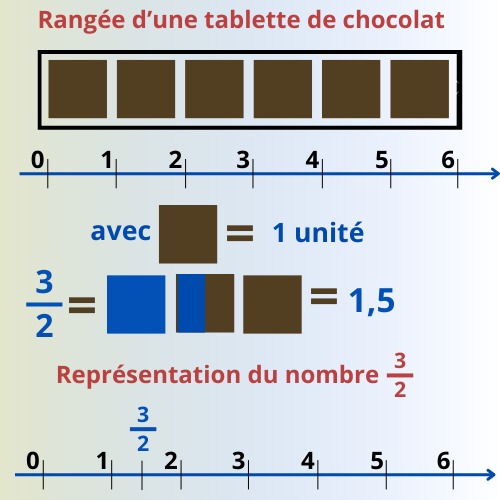
\includegraphics[width=0.60\linewidth]{Tablette de chocolat.png}
    \caption{Illustration de la fraction \(\frac{3}{2}\) comme 1 carré entier et une demi-unité sur la droite graduée.}
    \label{fig:enter-label}
\end{figure}

\subsubsection{\textcolor{green}{Opérations sur les fractions}}

\vspace{0.35cm}

\begin{tcolorbox}[colback=cyan!10!white, colframe=red!75!black, title=\textcolor{white}{Définitions et Règles}, 
                  sharp corners=southwest]
    \textcolor{black}{\textbf{Addition et Soustraction} : 
    Pour additionner ou soustraire des fractions, les dénominateurs doivent être identiques. Si ce n'est pas le cas, il faut trouver un dénominateur commun.}
    
    \vspace{5pt}
    
    \textcolor{black}{\textbf{Multiplication} :
    Pour multiplier deux fractions, multipliez les numérateurs entre eux et les dénominateurs entre eux.}
    
    \vspace{5pt}
    
    \textcolor{black}{\textbf{Division} :
    Pour diviser une fraction par une autre, multipliez la première fraction par l'inverse de la seconde.}
\end{tcolorbox}

\vspace{0.2cm}

\textcolor{purple}{Dans cette sous-section, nous allons explorer les règles et les méthodes pour effectuer des opérations sur les fractions.}

\vspace{0.2cm}

\begin{tcolorbox}[colback=orange!10!white, colframe=orange!75!black, title=\textcolor{white}{Exemples d'opérations}, sharp corners=southwest]
    \textcolor{purple}{\textbf{1. Addition de fractions avec dénominateurs identiques}}
    
    \[
    \frac{1}{4} + \frac{2}{4} = \frac{3}{4}
    \]
    
    \vspace{10pt}
    \textcolor{purple}{\textbf{2. Addition de fractions avec dénominateurs différents}}
    
    Trouvons un dénominateur commun pour \(\frac{1}{3}\) et \(\frac{1}{4}\).
    
    \[
    \frac{1}{3} + \frac{1}{4} = \frac{4}{12} + \frac{3}{12} = \frac{7}{12}
    \]
    
    \vspace{10pt}
    \textcolor{purple}{\textbf{3. Soustraction de fractions}}
    
    \[
    \frac{5}{6} - \frac{2}{6} = \frac{3}{6} = \frac{1}{2}
    \]
    
    \vspace{10pt}
    \textcolor{purple}{\textbf{4. Multiplication de fractions}}
    
    \[
    \frac{2}{3} \times \frac{4}{5} = \frac{8}{15}
    \]
    
    \vspace{10pt}
    \textcolor{purple}{\textbf{5. Division de fractions}}
    
    \[
    \frac{3}{4} \div \frac{2}{5} = \frac{3}{4} \times \frac{5}{2} = \frac{15}{8} = 1 \frac{7}{8}
    \]
    
    \vspace{10pt}
    \textcolor{purple}{\textbf{6. Simplification des fractions après opérations}}
    
    \[
    \frac{6}{8} = \frac{3}{4}
    \]
\end{tcolorbox}

\vspace{0.2cm}

\begin{tcolorbox}[colback=purple!10!white, colframe=yellow!75!black, title=\textcolor{white}{Application directe}, sharp corners=south, boxrule=0.8mm]
    \textbf{1. Addition de fractions avec dénominateurs différents}
    
    \[
    \frac{3}{7} + \frac{2}{5} = \_\_\_\_
    \]
    
    \vspace{10pt}
    
    \textbf{2. Soustraction de fractions}
    
    \[
    \frac{5}{8} - \frac{1}{8} = \_\_\_\_
    \]
    
    \vspace{10pt}
    
    \textbf{3. Multiplication de fractions}
    
    \[
    \frac{4}{9} \times \frac{3}{4} = \_\_\_\_
    \]
    
    \vspace{10pt}
    
    \textbf{4. Division de fractions}
    
    \[
    \frac{7}{10} \div \frac{2}{5} = \_\_\_\_
    \]
    
    \vspace{10pt}
    
    \textbf{5. Simplification après addition}
    
    \[
    \frac{2}{6} + \frac{1}{6} = \frac{3}{6} = \_\_\_\_
    \]
    
    \vspace{10pt}
    
    \textbf{6. Trouver un dénominateur commun}
    
    Additionnez les fractions suivantes :
    
    \[
    \frac{1}{2} + \frac{1}{3} = \_\_\_\_
    \]
    
    \vspace{10pt}
    
    \textbf{7. Multiplication et simplification}
    
    \[
    \frac{3}{5} \times \frac{5}{9} = \_\_\_\_
    \]
    
    \vspace{10pt}
    
    \textbf{8. Division et simplification}
    
    \[
    \frac{6}{7} \div \frac{3}{14} = \_\_\_\_
    \]
    
    \vspace{10pt}
    
    \textbf{9. Addition avec simplification}
    
    \[
    \frac{4}{12} + \frac{2}{12} = \_\_\_\_
    \]
    
    \vspace{10pt}
    
    \textbf{10. Problème pratique}
    
    Si une tarte est divisée en 8 parts égales et que vous en mangez \(\frac{3}{8}\), combien de parts reste-t-il ?
    
    \[
    \frac{3}{8} \text{ de la tarte a été mangée, il reste } \_\_\_\_ \text{ parts}
    \]
\end{tcolorbox}

\vspace{0.2cm}
\begin{tcolorbox}[colback=purple!10!white, colframe=yellow!75!black, title=\textcolor{white}{Exercices d'Application}, sharp corners=south, boxrule=0.8mm]
    \textbf{11.} Dessinez un cercle et divisez-le en 8 parts égales. Coloriez \(\frac{3}{8}\) du cercle en bleu.

    \textbf{12.} Si vous avez une pizza coupée en 12 parts égales et que vous en avez mangé 5, quelle fraction de la pizza reste-t-il?

    \textbf{13.} Complétez les fractions suivantes avec des fractions équivalentes : \(\frac{2}{4} = \_\_\_\_\_\), \(\frac{3}{6} = \_\_\_\_\_\).

    \textbf{14.} Convertissez les fractions suivantes en pourcentages : \(\frac{1}{2}\), \(\frac{3}{4}\), \(\frac{2}{5}\).

    \textbf{15.} Trouvez une fraction équivalente pour chaque fraction donnée : \(\frac{4}{10}\), \(\frac{5}{15}\), \(\frac{9}{12}\).

    \textbf{16.} Additionnez les fractions suivantes et simplifiez votre réponse : \(\frac{1}{4} + \frac{2}{4}\).

    \textbf{17.} Si un gâteau est coupé en 8 parts égales et que vous en mangez \(\frac{5}{8}\), quelle fraction du gâteau reste-t-il?

    \textbf{18.} Multipliez les fractions suivantes : \(\frac{1}{2} \times \frac{3}{5}\), \(\frac{2}{3} \times \frac{4}{7}\).

    \textbf{19.} Divisez \(\frac{3}{4}\) par \(\frac{1}{2}\) et simplifiez votre réponse.

    \textbf{20.} Identifiez les fractions équivalentes suivantes : \(\frac{3}{9} = \_\_\_\_\_\ \).

    \textbf{21.} Représentez la fraction \(\frac{5}{2}\) sur une droite graduée en utilisant une tablette de chocolat de 6 petits carrés alignés. Marquez les unités entières et la demi-unité.

    \textbf{22.} Représentez la fraction \(\frac{7}{3}\) de la même manière sur une droite graduée en plaçant une unité entière et une demi-unité.
\end{tcolorbox}

\vspace{0.2cm}
\begin{tcolorbox}[colback=orange!10!white, colframe=orange!75!black, title=\textcolor{white}{Comparaison des Fractions}, sharp corners=south, boxrule=0.8mm]
    \centering
    \begin{tabular}{|c|c|}
        \hline
        \textbf{Fraction} & \textbf{Proportions} \\
        \hline
        \(\frac{1}{2}\) & 50\% \\
        \hline
        \(\frac{1}{3}\) & 33.33\% \\
        \hline
        \(\frac{1}{4}\) & 25\% \\
        \hline
        \(\frac{1}{5}\) & 20\% \\
        \hline
        \(\frac{1}{6}\) & 16.67\% \\
        \hline
        \(\frac{1}{7}\) & 14.29\% \\
        \hline
        \(\frac{1}{8}\) & 12.5\% \\
        \hline
        \(\frac{1}{9}\) & 11.11\% \\
        \hline
        \(\frac{1}{10}\) & 10\% \\
        \hline
    \end{tabular}
\end{tcolorbox}

\vspace{0.2pt}

\begin{tcolorbox}[colback=blue!10!white, colframe=cyan!75!black, title=\textcolor{white}{Récapitulatif}, sharp corners=south, boxrule=0.8mm]
    En résumé :
    \begin{itemize}
        \item Les fractions représentent une partie d'un tout et sont composées d'un numérateur et d'un dénominateur.
        \item Les illustrations montrent comment les fractions se divisent visuellement dans un cercle.
        \item \textbf{Représentation sur une tablette de chocolat} : Une tablette de chocolat divisée en petits carrés permet de visualiser des fractions sur une droite graduée en utilisant chaque carré comme unité de mesure.
        \item \textbf{Addition et Soustraction} : Assurez-vous que les dénominateurs sont identiques avant d'additionner ou de soustraire les numérateurs.
        \item \textbf{Multiplication} : Multipliez les numérateurs entre eux et les dénominateurs entre eux.
        \item \textbf{Division} : Multipliez la première fraction par l'inverse de la seconde.
        \item \textbf{Simplification} : Réduisez les fractions après les opérations pour obtenir une forme simplifiée.
        \item \textbf{Dénominateur Commun} : Pour additionner ou soustraire des fractions avec des dénominateurs différents, trouvez un dénominateur commun.     
    \end{itemize}
\end{tcolorbox}


\subsection{\textcolor{red}{Proportionnalité}}

\subsubsection{\textcolor{green}{Définitions}}

\begin{tcolorbox}[colback=red!10!white, colframe=red!75!black, title=\textcolor{white}{Définition}, 
                  sharp corners=southwest]
    La \textbf{proportionnalité} est une relation entre deux grandeurs qui varient de manière constante l'une par rapport à l'autre. on dit que deux suites de nombres sont proportionnelles quand, en multipliant (ou en divisant) par une même constante non nulle, les termes de l'une on obtient les termes de l'autre. Le facteur constant entre l'une et l'autre de ces suites est appelé \textbf{coefficient de proportionnalité}.
\end{tcolorbox}

\vspace{0.2cm}

\begin{tcolorbox}[colback=orange!10!white, colframe=orange!75!black, title=\textcolor{white}{Exemples}, 
                  sharp corners=south]
    \textbf{Exemple 1 :} Imaginons que vous ayez une recette pour 4 personnes et qu'elle demande 200 grammes de farine. Si vous souhaitez préparer la recette pour 8 personnes, vous aurez besoin de 400 grammes de farine. Ici, la quantité de farine et le nombre de personnes sont proportionnels.

    \vspace{0.2cm}

    \textbf{Exemple 2 :} Vous conduisez une voiture à une vitesse constante de 60 km/h. Si vous doublez le temps de conduite, vous doublerez également la distance parcourue. La distance parcourue est proportionnelle au temps de conduite.
\end{tcolorbox}

\vspace{0.2cm}

\begin{tcolorbox}[colback=purple!10!white, colframe=purple!75!black, title=\textcolor{white}{Note}, 
                  sharp corners=south]
    \textcolor{purple}{La proportionnalité nous aide à comprendre comment deux choses changent ensemble de manière régulière. C'est comme si on gardait le même rapport entre elles tout le temps.}
\end{tcolorbox}

\vspace{0.2cm}

\begin{tcolorbox}[colback=green!10!white, colframe=green!75!black, title=\textcolor{white}{Remarque}, 
                  sharp corners=south]
    \textcolor{green}{Pour vérifier si deux grandeurs sont proportionnelles, vous pouvez diviser l'une par l'autre et voir si le rapport est toujours le même. Si oui, alors elles sont proportionnelles.}
\end{tcolorbox}

\vspace{0.5cm}

\textcolor{purple}{La proportionnalité est une notion que nous rencontrons fréquemment dans notre vie quotidienne. Par exemple, lorsque nous faisons des courses, nous pouvons comparer les prix des produits en utilisant leur coût par kilo ou par litre. Si deux produits ont le même prix par kilo, cela signifie que leur coût est proportionnel à leur poids.}

\vspace{0.2cm}

\textcolor{purple}{Pour mieux comprendre la proportionnalité, essayons quelques activités simples :}

\vspace{0.2cm}

\textcolor{purple}{\textbf{Activité 1 :} Vous avez une boîte de crayons qui contient 12 crayons pour un prix de 3 euros. Si vous souhaitez acheter 24 crayons, combien devrez-vous payer ? Utilisez la proportionnalité pour trouver la réponse.}

\vspace{0.2cm}

\textcolor{purple}{\textbf{Activité 2 :} Vous regardez un film avec une durée de 90 minutes. Si vous avez regardé 30 minutes du film, quelle fraction du film avez-vous regardée ? Comment pouvez-vous utiliser la proportionnalité pour vérifier votre réponse ?}

\vspace{0.2cm}

\textcolor{purple}{\textbf{Activité 3 :} Si une bouteille de jus de fruit de 1 litre coûte 2 euros, combien coûteront 3 bouteilles ? Vérifiez en utilisant la proportionnalité.}

\vspace{0.2cm}

\textcolor{purple}{Ces activités vous aideront à voir comment la proportionnalité est utilisée dans des situations réelles et comment vous pouvez l'appliquer pour résoudre des problèmes quotidiens.}

\vspace{0.2cm}

\textcolor{purple}{N'oubliez pas que la proportionnalité est une compétence très utile qui vous permet de maintenir un rapport constant entre deux grandeurs. Cela vous aidera non seulement dans vos études mais aussi dans de nombreux aspects de votre vie quotidienne !}

\subsubsection{\textcolor{green}{Tableaux de proportionnalité}}

\vspace{0.2cm}

\begin{tcolorbox}[colback=blue!10!white, colframe=red!75!black, title=\textcolor{white}{Définition}, 
                  sharp corners=south]
    Un \textbf{tableau de proportionnalité} est un outil utilisé pour organiser et résoudre des problèmes de proportionnalité. Il permet de comparer deux grandeurs et de déterminer des valeurs manquantes en utilisant le coefficient de proportionnalité.
\end{tcolorbox}

\vspace{0.2cm}

\textbf{Comment construire un tableau de proportionnalité ?}
\begin{itemize}
    \item Créez un tableau avec deux colonnes, une pour chaque grandeur à comparer.
    \item Inscrivez les valeurs connues dans les cases appropriées.
    \item Utilisez la proportionnalité pour compléter les valeurs manquantes.
\end{itemize}

\vspace{0.2cm}

\begin{tcolorbox}[colback=orange!10!white, colframe=orange!75!black, title=\textcolor{white}{Exemple 1}, 
                  sharp corners=south]
    Un paquet de 4 crayons coûte 2 euros. Nous voulons savoir combien coûteront 10 crayons.

    \[
    \begin{array}{|c|c|}
    \hline
    \text{Nombre de crayons} & \text{Coût (en euros)} \\
    \hline
    4 & 2 \\
    \hline
    10 & ? \\
    \hline
    \end{array}
    \]

    \textbf{Méthode :}
    \begin{itemize}
        \item Calculez le coefficient de proportionnalité : \(\frac{2}{4} = 0.5\) euros par crayon.
        \item Multipliez ce coefficient par le nombre de crayons désiré : \(0.5 \times 10 = 5\) euros.
    \end{itemize}

    \textbf{Tableau Complété :}
    \[
    \begin{array}{|c|c|}
    \hline
    \text{Nombre de crayons} & \text{Coût (en euros)} \\
    \hline
    4 & 2 \\
    \hline
    10 & 5 \\
    \hline
    \end{array}
    \]
\end{tcolorbox}

\vspace{0.2cm}

\begin{tcolorbox}[colback=purple!10!white, colframe=orange!75!black, title=\textcolor{white}{Exemple 2}, 
                  sharp corners=south]
    Un livre de 300 pages coûte 15 euros. Combien coûteront 450 pages ?

    \textbf{Étapes :}
    \begin{itemize}
        \item Créez un tableau pour comparer le nombre de pages et le prix :
    \end{itemize}

    \[
    \begin{array}{|c|c|}
    \hline
    \text{Nombre de pages} & \text{Prix (en euros)} \\
    \hline
    300 & 15 \\
    \hline
    450 & ? \\
    \hline
    \end{array}
    \]

    \textbf{Méthode de Résolution :}
    \begin{itemize}
        \item Calculez le coefficient de proportionnalité : \(\frac{15}{300} = 0.05\) euros par page.
        \item Multipliez ce coefficient par le nombre de pages désiré : \(0.05 \times 450 = 22.5\) euros.
    \end{itemize}

    \textbf{Tableau Complété :}
    \[
    \begin{array}{|c|c|}
    \hline
    \text{Nombre de pages} & \text{Prix (en euros)} \\
    \hline
    300 & 15 \\
    \hline
    450 & 22.5 \\
    \hline
    \end{array}
    \]
\end{tcolorbox}

\vspace{0.2cm}

\begin{tcolorbox}[colback=green!10!white, colframe=yellow!75!black, title=\textcolor{white}{Application directe}, 
                  sharp corners=south]
    \textbf{Exercice 1 :} Un paquet de 8 gommes coûte 4 euros. Complétez le tableau pour savoir combien coûteront 20 gommes.

    \[
    \begin{array}{|c|c|}
    \hline
    \text{Nombre de gommes} & \text{Coût (en euros)} \\
    \hline
    8 & 4 \\
    \hline
    20 & ? \\
    \hline
    \end{array}
    \]

    \textbf{Exercice 2 :} Un ticket de cinéma coûte 7 euros pour 1 film. Complétez le tableau pour savoir combien coûteront les billets pour 5 films.

    \[
    \begin{array}{|c|c|}
    \hline
    \text{Nombre de films} & \text{Coût (en euros)} \\
    \hline
    1 & 7 \\
    \hline
    5 & ? \\
    \hline
    \end{array}
    \]

    \textbf{Exercice 3 :} Un abonnement mensuel à une salle de sport coûte 30 euros pour 1 mois. Complétez le tableau pour savoir combien coûtera un abonnement de 6 mois.

    \[
    \begin{array}{|c|c|}
    \hline
    \text{Nombre de mois} & \text{Coût (en euros)} \\
    \hline
    1 & 30 \\
    \hline
    6 & ? \\
    \hline
    \end{array}
    \]

    \textbf{Exercice 4 :} Un paquet de 3 litres de lait coûte 2.4 euros. Complétez le tableau pour savoir combien coûteront 7 litres de lait.

    \[
    \begin{array}{|c|c|}
    \hline
    \text{Quantité (litres)} & \text{Coût (en euros)} \\
    \hline
    3 & 2.4 \\
    \hline
    7 & ? \\
    \hline
    \end{array}
    \]

    \textbf{Exercice 5 :} Un travailleur gagne 150 euros pour 20 heures de travail. Complétez le tableau pour savoir combien il gagnera pour 35 heures de travail.

    \[
    \begin{array}{|c|c|}
    \hline
    \text{Nombre d'heures} & \text{Salaire (en euros)} \\
    \hline
    20 & 150 \\
    \hline
    35 & ? \\
    \hline
    \end{array}
    \]

    \textbf{Exercice 6 :} Une machine produit 120 pièces en 4 heures. Complétez le tableau pour savoir combien de pièces seront produites en 6 heures.

    \[
    \begin{array}{|c|c|}
    \hline
    \text{Temps (heures)} & \text{Nombre de pièces} \\
    \hline
    4 & 120 \\
    \hline
    6 & ? \\
    \hline
    7 & ? \\
    \hline
    ? & 270 \\
    \hline
    10 & ? \\
    \hline
    \end{array}
    \]
\end{tcolorbox}

\vspace{0.2cm}

\begin{tcolorbox}[colback=blue!10!white, colframe=cyan!75!black, title=\textcolor{white}{Récapitulatif}, 
                  sharp corners=south]

    \begin{itemize}
        \item Un tableau de proportionnalité est un outil pour organiser les valeurs et résoudre des problèmes proportionnels.
        \item Il est constitué de lignes et de colonnes, chaque ligne représentant une paire de valeurs proportionnelles.
        \item Pour compléter un tableau, utilisez le coefficient de proportionnalité, qui est le rapport constant entre les valeurs.
        \item Vérifiez les résultats en calculant le produit du coefficient de proportionnalité par les valeurs connues ou en vérifiant si le rapport reste constant.
    \end{itemize}
\end{tcolorbox}

\vspace{0.25cm}

\subsection{\textcolor{red}{ Exercices et Corrections}}

\begin{tcolorbox}[colback=yellow!10!white, colframe=yellow!75!black, title=\textcolor{white}{\textbf{Exercices}}, sharp corners=south, boxrule=0.8mm]
    
    \textbf{Exercices sur les Fractions :}
    
    \vspace{5pt}
    
    \textbf{1.} Simplifiez les fractions suivantes :
    \[
    \frac{24}{36}, \quad \frac{15}{25}, \quad \frac{9}{12}
    \]
    
    \vspace{10pt}
    
    \textbf{2.} Effectuez les opérations suivantes et simplifiez le résultat :
    \[
    \frac{3}{4} + \frac{2}{4}, \quad \frac{5}{6} - \frac{1}{6}, \quad \frac{2}{3} \times \frac{3}{5}, \quad \frac{4}{7} \div \frac{2}{3}
    \]
    
    \vspace{10pt}
    
    \textbf{3.} Convertissez les fractions suivantes en pourcentages :
    \[
    \frac{1}{2}, \quad \frac{3}{5}, \quad \frac{7}{8}
    \]
    
    \vspace{10pt}
    
    \textbf{4.} Trouvez des fractions équivalentes aux suivantes :
    \[
    \frac{2}{3}, \quad \frac{4}{5}, \quad \frac{6}{9}
    \]
    
    \vspace{20pt}
    
    \textbf{Exercices sur la Proportionnalité :}
    
    \vspace{5pt}
    
    \textbf{5.} Un sac de pommes de terre pèse 5 kg et coûte 15 euros. Combien coûteront 8 kg de pommes de terre au même tarif ?
    
    \vspace{10pt}
    
    \textbf{6.} Une imprimante peut imprimer 180 pages en 3 heures. Combien de pages pourra-t-elle imprimer en 5 heures au même rythme ?
    
    \vspace{10pt}
    
    \textbf{7.} Complétez le tableau de proportionnalité suivant :
    
    \[
    \begin{array}{|c|c|}
    \hline
    \text{Nombre de crayons} & \text{Coût (en euros)} \\
    \hline
    6 & 3 \\
    \hline
    10 & ? \\
    \hline
    15 & 7.5 \\
    \hline
    ? & 12 \\
    \hline
    \end{array}
    \]
    \end{tcolorbox}
    
    \vspace{20pt}

    \begin{tcolorbox}[colback=yellow!10!white, colframe=yellow!75!black, title=\textcolor{white}{\textbf{Exercices}}, sharp corners=south, boxrule=0.8mm]
    
    \textbf{Exercices sur les Tableaux de Proportionnalité :}
    
    \vspace{5pt}
    
    \textbf{8.} Un tableau de proportionnalité est donné pour la relation entre le nombre d'heures travaillées et le salaire gagné. Complétez les cases manquantes.
    
    \[
    \begin{array}{|c|c|}
    \hline
    \text{Heures travaillées} & \text{Salaire (en euros)} \\
    \hline
    4 & 120 \\
    \hline
    6 & ? \\
    \hline
    10 & 300 \\
    \hline
    ? & 450 \\
    \hline
    \end{array}
    \]
    
    \vspace{10pt}
    
    \textbf{9.} Remplissez le tableau de proportionnalité pour la recette de cuisine :
    
    \[
    \begin{array}{|c|c|}
    \hline
    \text{Nombre de personnes} & \text{Quantité de sucre (en grammes)} \\
    \hline
    2 & 100 \\
    \hline
    5 & ? \\
    \hline
    8 & 400 \\
    \hline
    ? & 250 \\
    \hline
    \end{array}
    \]
    
    \vspace{20pt}
    
    \textbf{Exercices Combinés (Fractions et Proportionnalité) :}
    
    \vspace{5pt}
    
    \textbf{10.} Une recette nécessite \(\frac{3}{4}\) de tasse de sucre pour 6 muffins. Combien de tasses de sucre seront nécessaires pour faire 18 muffins ?
    
    \vspace{10pt}
    
    \textbf{11.} Un cycliste parcourt \(\frac{5}{6}\) de la distance totale en 2 heures. Si la distance totale est de 36 km, quelle distance a-t-il parcourue en 2 heures et combien de temps lui faudra-t-il pour parcourir la distance totale au même rythme ?
    
\end{tcolorbox}

\vspace{5pt}

\begin{tcolorbox}[colback=green!10!white, colframe=green!75!black, title=\textcolor{white}{\textbf{Corrections}}, sharp corners=south, boxrule=0.8mm]
    
    \textbf{Corrections des Exercices sur les Fractions :}
    
    \vspace{5pt}
    
    \textbf{1.} Simplifications des fractions :
    \[
    \frac{24}{36} = \frac{2}{3}, \quad \frac{15}{25} = \frac{3}{5}, \quad \frac{9}{12} = \frac{3}{4}
    \]
    
    \vspace{10pt}
    
    \textbf{2.} Résultats des opérations :
    \[
    \frac{3}{4} + \frac{2}{4} = \frac{5}{4} = 1.25, \quad \frac{5}{6} - \frac{1}{6} = \frac{4}{6} = \frac{2}{3}, \quad \frac{2}{3} \times \frac{3}{5} = \frac{6}{15} = \frac{2}{5}, \quad \frac{4}{7} \div \frac{2}{3} = \frac{4}{7} \times \frac{3}{2} = \frac{12}{14} = \frac{6}{7}
    \]
    
    \vspace{10pt}
    
    \textbf{3.} Conversion en pourcentages :
    \[
    \frac{1}{2} = 50\%, \quad \frac{3}{5} = 60\%, \quad \frac{7}{8} = 87.5\%
    \]
    
    \vspace{10pt}
    
    \textbf{4.} Fractions équivalentes :
    \[
    \frac{2}{3} = \frac{4}{6} = \frac{6}{9}, \quad \frac{4}{5} = \frac{8}{10} = \frac{12}{15}, \quad \frac{6}{9} = \frac{12}{18} = \frac{18}{27}
    \]
\end{tcolorbox}

\begin{tcolorbox}[colback=green!10!white, colframe=green!75!black, title=\textcolor{white}{\textbf{Corrections}}, sharp corners=south, boxrule=0.8mm]
    
    \textbf{Corrections des Exercices sur la Proportionnalité :}
    
    \vspace{5pt}
    
    \textbf{5.} Coût pour 8 kg :
    \[
    \text{Prix pour 8 kg} = \left( \frac{15 \, \text{euros}}{5 \, \text{kg}} \right) \times 8 \, \text{kg} = 24 \, \text{euros}
    \]
    
    \vspace{10pt}
    
    \textbf{6.} Pages imprimées en 5 heures :
    \[
    \text{Pages en 5 heures} = \left( \frac{180 \, \text{pages}}{3 \, \text{heures}} \right) \times 5 \, \text{heures} = 300 \, \text{pages}
    \]
    
    \vspace{10pt}
    
    \textbf{7.} Tableau de proportionnalité complété :
    
    \[
    \begin{array}{|c|c|}
    \hline
    \text{Nombre de crayons} & \text{Coût (en euros)} \\
    \hline
    6 & 3 \\
    \hline
    10 & 5 \\
    \hline
    15 & 7.5 \\
    \hline
    10 & 5 \\
    \hline
    \end{array}
    \]
    
    \vspace{20pt}
    
    \textbf{Corrections des Exercices sur les Tableaux de Proportionnalité :}
    
    \vspace{5pt}
    
    \textbf{8.} Tableau complété :
    
    \[
    \begin{array}{|c|c|}
    \hline
    \text{Heures travaillées} & \text{Salaire (en euros)} \\
    \hline
    4 & 120 \\
    \hline
    6 & 180 \\
    \hline
    10 & 300 \\
    \hline
    15 & 450 \\
    \hline
    \end{array}
    \]
    
    \vspace{10pt}
    
    \textbf{9.} Tableau complété pour la recette :
    
    \[
    \begin{array}{|c|c|}
    \hline
    \text{Nombre de personnes} & \text{Quantité de sucre (en grammes)} \\
    \hline
    2 & 100 \\
    \hline
    5 & 250 \\
    \hline
    8 & 400 \\
    \hline
    10 & 500 \\
    \hline
    \end{array}
    \]
    
    \vspace{20pt}
    
    \textbf{Corrections des Exercices Combinés :}
    
    \vspace{5pt}
    
    \textbf{10.} Tasses de sucre pour 18 muffins :
    \[
    \text{Pour 18 muffins} = \frac{3}{4} \times 3 = \frac{9}{4} = 2.25 \, \text{tasses}
    \]
    
    \vspace{10pt}
    
    \textbf{11.} Distance parcourue et temps :
    \[
    \text{Distance parcourue en 2 heures} = \frac{5}{6} \times 36 \, \text{km} = 30 \, \text{km}
    \]
    \[
    \text{Temps pour la distance totale} = \frac{36 \, \text{km}}{15 \, \text{km/h}} = 2.4 \, \text{heures} \approx 2 \, \text{heures} \, 24 \, \text{minutes}
    \]
    
\end{tcolorbox}

\section{\textcolor{blue}{Chapitre 4: Géométrie}}

\subsection{\textcolor{red}{Distances et Droites}}

\subsubsection{\textcolor{green}{Distances}}

\begin{tcolorbox}[colback=red!10!white, colframe=red!75!black, title=\textcolor{white}{Définitions}, sharp corners=south]
    La \textbf{distance} est la longueur entre deux points. Pour trouver cette distance, on utilise la formule :
    \[
    d = \sqrt{(x_2 - x_1)^2 + (y_2 - y_1)^2}
    \]
    où \((x_1, y_1)\) et \((x_2, y_2)\) sont les coordonnées des points.
\end{tcolorbox}

\vspace{0.2cm}

\begin{tcolorbox}[colback=orange!10!white, colframe=orange!75!black, title=\textcolor{white}{Exemple d'application}, sharp corners=south]
    \textbf{Exemple :} Trouvons la distance entre les points \(A(1, 2)\) et \(B(4, 6)\).
    \[
    d = \sqrt{(4 - 1)^2 + (6 - 2)^2} = \sqrt{3^2 + 4^2} = \sqrt{9 + 16} = \sqrt{25} = 5
    \]
\end{tcolorbox}

\vspace{0.2cm}

\begin{tcolorbox}[colback=blue!10!white, colframe=blue!75!black, title=\textcolor{white}{Illustration}, sharp corners=south]
    \begin{center}
    \begin{tikzpicture}[scale=0.8]
        \draw[->] (-1, 0) -- (5, 0) node[right] {\(x\)};
        \draw[->] (0, -1) -- (0, 7) node[above] {\(y\)};
        \foreach \x in {1, 2, 3, 4} \draw (\x, 0) -- (\x, 0.1) node[above] {\x};
        \foreach \y in {1, 2, 3, 4, 5, 6} \draw (0, \y) -- (0.1, \y) node[right] {\y};
        \draw[fill=red] (1, 2) circle (3pt) node[above right] {\(A(1, 2)\)};
        \draw[fill=red] (4, 6) circle (3pt) node[above right] {\(B(4, 6)\)};
        \draw[dashed] (1, 2) -- (4, 6) node[midway, above right] {\(d = 5\)};
        \node at (2.5, 4) {Distance entre \(A\) et \(B\)};
    \end{tikzpicture}
    \end{center}
\end{tcolorbox}

\vspace{0.2cm}

\subsubsection{\textcolor{green}{Droites}}

\begin{tcolorbox}[colback=red!10!white, colframe=red!75!black, title=\textcolor{white}{Définitions}, sharp corners=south]
    Il existe plusieurs types de droites :
    \begin{itemize}
        \item \textbf{Droite :} s'étend indéfiniment dans les deux sens. 
        \item \textbf{Demi-droite :} part d'un point et s'étend indéfiniment dans un sens. 
        \item \textbf{Segment de droite :} a deux points d'extrémité et a une longueur finie.
    \end{itemize}
\end{tcolorbox}

\vspace{0.2cm}

\begin{tcolorbox}[colback=red!10!white, colframe=red!75!black, title=\textcolor{white}{Définitions}, sharp corners=south]
    \begin{itemize}
        \item \textbf{Droites parallèles :} Deux droites sont parallèles si elles ne se rencontrent jamais, quelle que soit leur extension.
        \item \textbf{Droites perpendiculaires :} Deux droites sont perpendiculaires si elles se croisent en formant un angle droit (90°).
        \item \textbf{Droites sécantes :} Deux droites sont sécantes si elles se rencontrent en un point.
        \item \textbf{Droites confondues :} Deux droites sont confondues si elles se superposent exactement, c’est-à-dire qu’elles ont les mêmes points.
    \end{itemize}
\end{tcolorbox}

\vspace{0.2cm}

\begin{tcolorbox}[colback=orange!10!white, colframe=orange!75!black, title=\textcolor{white}{Exemple de traçage}, sharp corners=south]
    \textbf{Exemple :} Pour tracer un segment de droite entre deux points \(A\) et \(B\) :
    \begin{enumerate}
        \item Placez les points \(A\) et \(B\) sur la feuille.
        \item Utilisez une règle pour relier ces deux points par une ligne droite.
    \end{enumerate}
\end{tcolorbox}

\vspace{0.2cm}

\subsubsection{\textcolor{green}{Illustrations des droites parallèles, perpendiculaires, sécantes et confondues}}

\vspace{0.2cm}

\begin{tcolorbox}[colback=blue!10!white, colframe=blue!75!black, title=\textcolor{white}{Illustration des droites parallèles}, sharp corners=south]
    \begin{center}
    \begin{tikzpicture}
        \draw[thick] (0, 0) -- (5, 0) node[below] {\(d_1\)};
        \draw[thick] (0, 1) -- (5, 1) node[below] {\(d_2\)};
        \node at (2.5, 1.5) {Droites parallèles};
    \end{tikzpicture}
    \end{center}
\end{tcolorbox}

\vspace{0.2cm}

\begin{tcolorbox}[colback=blue!10!white, colframe=blue!75!black, title=\textcolor{white}{Illustration des droites perpendiculaires}, sharp corners=south]
    \begin{center}
    \begin{tikzpicture}
        \draw[thick] (0, 0) -- (5, 0) node[below] {\(d_1\)};
        \draw[thick] (2.5, -2) -- (2.5, 2) node[right] {\(d_2\)};
        \node at (3.5, -1.5) {Droites perpendiculaires};
        \node at (2.5, -0.5) {90°};
    \end{tikzpicture}
    \end{center}
\end{tcolorbox}

\vspace{0.2cm}

\begin{tcolorbox}[colback=blue!10!white, colframe=blue!75!black, title=\textcolor{white}{Illustration des droites sécantes}, sharp corners=south]
    \begin{center}
    \begin{tikzpicture}
        \draw[thick] (0, 0) -- (5, 2) node[below] {\(d_1\)};
        \draw[thick] (0, 2) -- (5, 0) node[below] {\(d_2\)};
        \node at (3, 1) {Droites sécantes};
    \end{tikzpicture}
    \end{center}
\end{tcolorbox}

\vspace{0.2cm}

\begin{tcolorbox}[colback=blue!10!white, colframe=blue!75!black, title=\textcolor{white}{Illustration des droites confondues}, sharp corners=south]
    \begin{center}
    \begin{tikzpicture}
        \draw[thick] (0, 0) -- (5, 0) node[below] {\(d_1\)};
        \draw[thick] (0, 0) -- (5, 0) node[above] {\(d_2\)};
        \node at (2.5, 1.5) {Droites confondues};
    \end{tikzpicture}
    \end{center}
\end{tcolorbox}

\vspace{0.2cm}

\begin{tcolorbox}[colback=yellow!10!white, colframe=yellow!75!black, title=\textcolor{white}{Application directe}, sharp corners=south]
    \textbf{Exercice 3 :} Tracez deux droites parallèles \(d_1\) et \(d_2\) et vérifiez qu'elles ne se coupent pas.

    \textbf{Exercice 4 :} Tracez deux droites perpendiculaires et mesurez l'angle entre elles pour vérifier qu'il est de 90°.

    \textbf{Exercice 5 :} Tracez deux droites sécantes et trouvez leur point d'intersection.

    \textbf{Exercice 6 :} Tracez deux droites confondues et expliquez pourquoi elles sont identiques.
\end{tcolorbox}

\vspace{0.5cm}

\subsection{\textcolor{red}{Figures: Carrés, Rectangles, Triangles et Cercles}}

\subsubsection{\textcolor{green}{Carrés et Rectangles}}

\begin{tcolorbox}[colback=red!10!white, colframe=red!75!black, title=\textcolor{white}{Définitions}, sharp corners=south]
    - Un \textbf{carré} a quatre côtés égaux et quatre angles droits (90°). \\
    - Un \textbf{rectangle} a deux paires de côtés égaux et quatre angles droits.
\end{tcolorbox}

\vspace{0.2cm}

\begin{tcolorbox}[colback=orange!10!white, colframe=orange!75!black, title=\textcolor{white}{Exemple de traçage}, sharp corners=south]
    \textbf{Exemple :} Pour tracer un carré de côté 4 cm :
    \begin{enumerate}
        \item Tracez un segment de 4 cm avec une règle.
        \item À chaque extrémité, utilisez l'équerre pour former un angle droit (90°) et tracez 4 cm.
        \item Reliez les points pour former le carré.
    \end{enumerate}
\end{tcolorbox}

\textbf{Résolution :}

\begin{enumerate}
    \item \textbf{Tracez un segment de 4 cm :}
    \begin{itemize}
        \item Prenez une règle et placez-la sur votre feuille.
        \item Marquez un point \(A\) à 0 cm et un point \(B\) à 4 cm.
        \item Reliez les deux points pour obtenir le segment \(AB\).
    \end{itemize}

    \item \textbf{Formez des angles droits :}
    \begin{itemize}
        \item Placez l'équerre à l'une des extrémités (point \(A\)).
        \item Tracez une ligne perpendiculaire au segment \(AB\) en utilisant l'équerre pour créer l'angle droit, jusqu'à 4 cm. Marquez ce point \(C\).
        \item Répétez cette étape à l'autre extrémité (point \(B\)) pour tracer une ligne perpendiculaire jusqu'à 4 cm. Marquez ce point \(D\).
    \end{itemize}

    \item \textbf{Reliez les points :}
    \begin{itemize}
        \item Tracez un segment entre \(C\) et \(D\).
        \item Ensuite, reliez \(C\) à \(D\) pour former le carré. Vous devriez avoir un carré \(ABCD\).
    \end{itemize}
\end{enumerate}

\textbf{Illustration :}
\begin{tcolorbox}[colback=blue!10!white, colframe=blue!75!black, title=\textcolor{white}{Illustration}, sharp corners=south]
    \begin{center}
    \begin{tikzpicture}
        % Tracer le carré
        \draw[thick] (0, 0) -- (4, 0) -- (4, 4) -- (0, 4) -- cycle;
        
        % Points A, B, C, D
        \foreach \x/\y/\name in {0/0/A, 4/0/B, 4/4/C, 0/4/D} 
            \draw[fill=red] (\x, \y) circle (3pt) node[below right] {\textbf{\name}};
        
        % Indication des côtés
        \node at (2, -0.5) {Côté de 4 cm};
        \node at (4.5, 2) {Côté de 4 cm};
        \node at (-0.5, 2) {Côté de 4 cm};
        \node at (2, 4.5) {Côté de 4 cm};
    \end{tikzpicture}
    \end{center}
\end{tcolorbox}

\vspace{0.2cm}

\begin{tcolorbox}[colback=yellow!10!white, colframe=yellow!75!black, title=\textcolor{white}{Application directe}, sharp corners=south]
    \textbf{Exercice 1 :} Tracez un rectangle de longueur 6 cm et de largeur 3 cm.

    \textbf{Exercice 2 :} Tracez un carré de côté 5 cm.
\end{tcolorbox}

\subsubsection{\textcolor{green}{Triangles}}

\begin{tcolorbox}[colback=red!10!white, colframe=red!75!black, title=\textcolor{white}{Définitions}, sharp corners=south]
    Un \textbf{triangle} a trois côtés. La somme de ses angles est toujours égale à 180°.
\end{tcolorbox}

\vspace{0.2cm}

\begin{tcolorbox}[colback=orange!10!white, colframe=orange!75!black, title=\textcolor{white}{Exemple de traçage}, sharp corners=south]
    \textbf{Exemple :} Pour tracer un triangle :
    \begin{enumerate}
        \item Tracez un segment de 5 cm.
        \item Placez un point à 3 cm du premier point et un autre point à 4 cm du second point, formant un triangle.
        \item Reliez les points pour créer le triangle.
    \end{enumerate}
\end{tcolorbox}

\vspace{0.2cm}

\textbf{Résolution :}

\begin{enumerate}
    \item \textbf{Tracez un segment de 5 cm :}
    \begin{itemize}
        \item Prenez votre règle et tracez un segment horizontal de 5 cm. Marquez les extrémités de ce segment par les points \(A\) et \(B\).
        \item Vérifiez que le segment mesure exactement 5 cm pour garantir la précision du triangle.
    \end{itemize}

    \item \textbf{Placez un point à 3 cm du premier point :}
    \begin{itemize}
        \item À partir du point \(A\), mesurez 3 cm à l'aide de votre règle et marquez ce point comme \(C\). 
        \item Ce point \(C\) doit être hors du segment \(AB\) pour que les points puissent former un triangle.
    \end{itemize}

    \item \textbf{Placez un autre point à 4 cm du second point :}
    \begin{itemize}
        \item À partir du point \(B\), mesurez 4 cm pour trouver un point \(D\). Assurez-vous que ce point est également situé de manière à ce que les trois points ne soient pas alignés.
    \end{itemize}

    \item \textbf{Reliez les points pour créer le triangle :}
    \begin{itemize}
        \item Reliez les points \(A\), \(C\), et \(B\) pour former le triangle \(ABC\).
        \item Utilisez une règle pour tracer les segments \(AC\) et \(BC\).
    \end{itemize}
\end{enumerate}

\textbf{Illustration :}
\begin{tcolorbox}[colback=blue!10!white, colframe=blue!75!black, title=\textcolor{white}{Illustration}, sharp corners=south]
    \begin{center}
    \begin{tikzpicture}
        \draw[thick] (0, 0) -- (3, 4) -- (5, 0) -- cycle;
        \foreach \x/\y in {0/0, 3/4, 5/0} \draw[fill=red] (\x, \y) circle (3pt);
        \node at (2.5, 4.5) {Triangle};
        \node at (2.5, -0.5) {La somme des angles = 180°};
        \node at (0, -0.5) {A};
        \node at (3, 4.5) {C};
        \node at (5, -0.5) {B};
    \end{tikzpicture}
    \end{center}
\end{tcolorbox}

\vspace{0.2cm}

\begin{tcolorbox}[colback=yellow!10!white, colframe=yellow!75!black, title=\textcolor{white}{Application directe}, sharp corners=south]
    \textbf{Exercice 1 :} Tracez un triangle équilatéral dont les côtés mesurent 4 cm.

    \textbf{Exercice 2 :} Calculez la somme des angles d’un triangle que vous avez tracé.
\end{tcolorbox}

\vspace{0.5cm}

\subsubsection{\textcolor{green}{Cercle}}

\begin{tcolorbox}[colback=red!10!white, colframe=red!75!black, title=\textcolor{white}{Définitions}, sharp corners=south]
    Un \textbf{cercle} est l'ensemble des points à une distance donnée (le \textbf{rayon}) d'un point central (le \textbf{centre}).
    Le \textbf{diamètre} est le double du rayon et passe par le centre.
\end{tcolorbox}

\vspace{0.2cm}

\begin{tcolorbox}[colback=orange!10!white, colframe=orange!75!black, title=\textcolor{white}{Exemple de traçage}, sharp corners=south]
    \textbf{Exemple :} Pour tracer un cercle :
    \begin{enumerate}
        \item Placez le compas au centre du cercle.
        \item Ouvrez-le à la distance souhaitée pour le rayon.
        \item Faites tourner le compas pour tracer le cercle.
    \end{enumerate}
\end{tcolorbox}

\textbf{Résolution :}

\begin{enumerate}
    \item \textbf{Placez le compas au centre du cercle :}
    \begin{itemize}
        \item Choisissez un point sur votre feuille. Ce point sera le centre du cercle, que nous allons appeler \(O\).
        \item Positionnez la pointe du compas sur ce point \(O\). La pointe doit être stable et ne pas bouger pour assurer un cercle bien tracé.
    \end{itemize}

    \item \textbf{Ouvrez le compas à la distance souhaitée pour le rayon :}
    \begin{itemize}
        \item Écartez les deux branches du compas jusqu'à obtenir la distance souhaitée pour le rayon. Par exemple, si vous voulez un cercle de rayon 3 cm, ouvrez le compas à 3 cm entre la pointe et le crayon.
        \item Vérifiez que le compas est bien ouvert à la bonne mesure pour obtenir un cercle précis.
    \end{itemize}

    \item \textbf{Faites tourner le compas pour tracer le cercle :}
    \begin{itemize}
        \item En gardant la pointe du compas sur le point \(O\), faites tourner doucement le compas à 360° pour tracer le cercle.
        \item Assurez-vous que le crayon reste en contact avec le papier tout au long du mouvement pour former un cercle continu.
    \end{itemize}
\end{enumerate}

\textbf{Illustration :}
\begin{tcolorbox}[colback=blue!10!white, colframe=blue!75!black, title=\textcolor{white}{Illustration}, sharp corners=south]
    \begin{center}
    \begin{tikzpicture}
        % Tracer le cercle
        \draw[thick] (0,0) circle (3cm); % Cercle de rayon 3 cm
        
        % Centre O
        \fill[red] (0,0) circle (3pt) node[below right] {\textbf{O}};
        
        % Indication du rayon
        \draw[->] (0,0) -- (3,0) node[midway, above] {3 cm};
        
        % Indication du compas
        \node at (2, 2) {Compas ouvert};
    \end{tikzpicture}
    \end{center}
\end{tcolorbox}

\vspace{0.2cm}

\begin{tcolorbox}[colback=yellow!10!white, colframe=yellow!75!black, title=\textcolor{white}{Application directe}, sharp corners=south]
    \textbf{Exercice 1 :} Tracez un cercle de rayon 3 cm.

    \textbf{Exercice 2 :} Identifiez le centre et le rayon du cercle que vous avez tracé.
\end{tcolorbox}

\vspace{0.5cm}

\subsection{\textcolor{red}{Angles et Mesures}}

\subsubsection{\textcolor{green}{Définition d'un angle}}

\begin{tcolorbox}[colback=red!10!white, colframe=red!75!black, title=\textcolor{white}{Définition : Angle}, sharp corners=south]
    Un \textbf{angle} est formé par deux demi-droites qui se rencontrent en un point appelé le \textbf{sommet} de l'angle. Les deux demi-droites qui forment l'angle sont appelées les \textbf{côtés} de l'angle. L'ouverture entre les deux côtés est mesurée en \textbf{degrés (°)}.
\end{tcolorbox}

\begin{tcolorbox}[colback=purple!10!white, colframe=purple!75!black, title=\textcolor{white}{Note}, sharp corners=south]
    Il existe plusieurs types d'angles :
    \begin{itemize}
        \item \textbf{Angle aigu} : un angle inférieur à 90°.
        \item \textbf{Angle droit} : un angle exactement égal à 90°.
        \item \textbf{Angle obtus} : un angle supérieur à 90° mais inférieur à 180°.
        \item \textbf{Angle plat} : un angle de 180°.
    \end{itemize}
\end{tcolorbox}

\vspace{0.2cm}

\begin{tcolorbox}[colback=red!10!white, colframe=red!75!black, title=\textcolor{white}{Propriété : Somme des angles dans un triangle}, sharp corners=south]
    Dans un \textbf{triangle}, la somme des mesures des trois angles est toujours égale à \textbf{180°}.
\end{tcolorbox}

\vspace{0.2cm}

\begin{tcolorbox}[colback=orange!10!white, colframe=orange!75!black, title=\textcolor{white}{Exemple de vérification}, sharp corners=south]
    \textbf{Exemple :} Pour vérifier que la somme des angles dans un triangle est bien égale à 180° :
    \begin{enumerate}
        \item Tracez un triangle quelconque avec une règle.
        \item Mesurez les trois angles avec un rapporteur.
        \item Additionnez les trois mesures d'angles. Le résultat doit être égal à 180°.
    \end{enumerate}
\end{tcolorbox}

\vspace{0.2cm}

\subsubsection{\textcolor{green}{Mesurer un angle avec un rapporteur}}

\begin{tcolorbox}[colback=orange!10!white, colframe=orange!75!black, title=\textcolor{white}{Exemple de mesure d'angle}, sharp corners=south]
    \textbf{Exemple :} Pour mesurer un angle avec un rapporteur :
    \begin{enumerate}
        \item Placez le centre du rapporteur sur le sommet de l'angle.
        \item Alignez une des lignes de l'angle avec la ligne de 0° du rapporteur.
        \item Lisez la mesure de l'angle où l'autre ligne de l'angle coupe l'échelle du rapporteur. Cette valeur vous donne la mesure de l'angle en degrés.
    \end{enumerate}
\end{tcolorbox}

\begin{tcolorbox}[colback=blue!10!white, colframe=blue!75!black, title=\textcolor{white}{Illustration : Types d'angles}, sharp corners=south]
    \begin{center}
    \begin{tikzpicture}
        % Angle droit
        \draw[thick] (0,0) -- (2,0);
        \draw[thick] (0,0) -- (0,2);
        \draw (0.4,0.4) node {90°};
        \draw[fill=red] (0,0) circle (3pt);
        \node at (-0.5, 0.2) {Sommet};
        \node at (1, -0.3) {Côté};
        \node at (-0.3, 1) {Côté};

        % Angle aigu
        \draw[thick] (4,0) -- (6,0);
        \draw[thick] (4,0) -- (5.5,1.5);
        \draw (5,0.3) node {60°};
        \draw[fill=red] (4,0) circle (3pt);
        \node at (3.5, 0.2) {Sommet};
        \node at (5, -0.3) {Côté};

        % Angle obtus corrigé à 120 degrés
        \draw[thick] (8,0) -- (10,0);
        \draw[thick] (8,0) -- ++(120:2); % Angle de 120 degrés
        \draw (9.2, 0.7) node {120°};
        \draw[fill=red] (8,0) circle (3pt);
        \node at (7.5, 0.2) {Sommet};
        \node at (9, -0.3) {Côté};
    \end{tikzpicture}
    \end{center}
\end{tcolorbox}

\vspace{0.2cm}

\textbf{Erreurs fréquentes à éviter} :
\begin{itemize}
    \item Ne pas confondre un angle aigu et un angle obtus : l'angle aigu est plus petit que l'angle droit, tandis que l'angle obtus est plus grand.
    \item Lors de la mesure, assurez-vous d'utiliser le bon côté du rapporteur, car il a deux échelles (de 0° à 180° et de 180° à 0°).
\end{itemize}

\vspace{0.2cm}

\begin{tcolorbox}[colback=yellow!10!white, colframe=yellow!75!black, title=\textcolor{white}{Exercice d'application 1}, sharp corners=south]
    \textbf{Exercice 1 :} Mesurez les angles suivants avec un rapporteur et identifiez s'ils sont aigus, droits ou obtus :
    \begin{itemize}
        \item \textbf{Un angle de 45° :}
        \begin{center}
        \begin{tikzpicture}
            \draw[thick] (0,0) -- (3,0) node[right] {};
            \draw[thick] (0,0) -- (2.12,2.12) node[above] {};
            \draw (0.6,0) arc[start angle=0,end angle=45,radius=0.6];
            \node at (1, 0.3) {$45^\circ$};
        \end{tikzpicture}
        \end{center}
        
        \item \textbf{Un angle de 135° :}
        \begin{center}
        \begin{tikzpicture}
            \draw[thick] (0,0) -- (3,0) node[right] {};
            \draw[thick] (0,0) -- (-2,2) node[above] {};
            \draw (0.6,0) arc[start angle=0,end angle=135,radius=0.6];
            \node at (1.1, 0.4) {$135^\circ$};
        \end{tikzpicture}
        \end{center}
    \end{itemize}
\end{tcolorbox}


\begin{tcolorbox}[colback=yellow!10!white, colframe=yellow!75!black, title=\textcolor{white}{Exercice d'application 2}, sharp corners=south]
    \textbf{Exercice 2 :} Tracez deux angles droits, un angle aigu et un angle obtus. Utilisez un rapporteur pour vérifier les mesures.
\end{tcolorbox}

\vspace{0.2cm}

\begin{tcolorbox}[colback=yellow!10!white, colframe=yellow!75!black, title=\textcolor{white}{Exercice d'application 3}, sharp corners=south]
    \textbf{Exercice 3 :} Tracez un triangle équilatéral (trois côtés égaux). Mesurez ses angles. Que remarquez-vous ?
\end{tcolorbox}

\begin{tcolorbox}[colback=cyan!10!white, colframe=cyan!75!black, title=\textcolor{white}{Récapitulatif}, sharp corners=south]
    - Un \textbf{angle} est formé de deux côtés partant d'un même point appelé sommet. \\
    - Les angles se mesurent en \textbf{degrés (°)}. \\
    - Les principaux types d'angles sont : \textbf{angle aigu} (moins de 90°), \textbf{angle droit} (90°), et \textbf{angle obtus} (plus de 90°). \\
    - La \textbf{somme des angles dans un triangle} est toujours égale à \textbf{180°}. \\
    - Pour mesurer un angle, on utilise un \textbf{rapporteur}. \\
    - Utilisez toujours une règle et un rapporteur pour tracer et vérifier les angles.
\end{tcolorbox}

\subsection{\textcolor{red}{Géométrie de l'Espace: Solides et Volumes}}

\subsubsection{\textcolor{green}{Solides de base}}

\begin{tcolorbox}[colback=red!10!white, colframe=red!75!black, title=\textcolor{white}{Définition : Solide}, sharp corners=south]
    Un \textbf{solide} est une figure géométrique en trois dimensions qui occupe un espace. Les solides ont une longueur, une largeur et une hauteur.
\end{tcolorbox}

Les solides les plus courants en géométrie de l'espace sont le cube, le pavé droit, la pyramide, le cylindre, le cône et la sphère. Ces solides ont des propriétés spécifiques que nous allons découvrir.

\begin{tcolorbox}[colback=orange!10!white, colframe=orange!75!black, title=\textcolor{white}{Exemples de solides}, sharp corners=south]
    \begin{enumerate}
        \item \textbf{Le cube} : Toutes ses faces sont des carrés, et ses arêtes ont la même longueur.
        \item \textbf{Le pavé droit} : C'est un solide ayant des faces rectangulaires.
        \item \textbf{La pyramide} : Elle a une base polygonale et des faces triangulaires qui se rejoignent à un sommet.
        \item \textbf{Le cylindre} : Il a deux bases circulaires identiques et une surface latérale courbe.
        \item \textbf{Le cône} : Il a une base circulaire et une face courbe qui rejoint un sommet.
        \item \textbf{La sphère} : C'est un solide parfaitement rond, comme une balle.
    \end{enumerate}
\end{tcolorbox}

\begin{figure}[H]
    \centering
    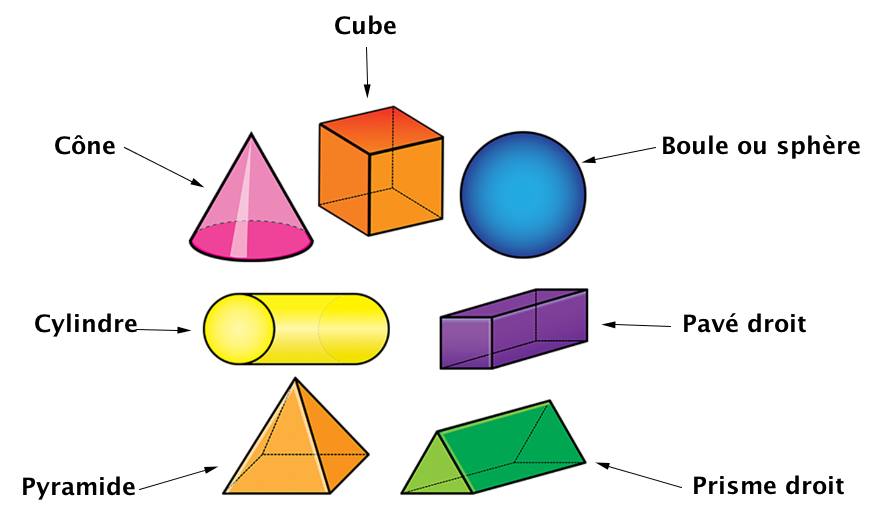
\includegraphics[width=0.75\linewidth]{les_solides.png}
    \caption{Les solides de base}
    \label{fig:enter-label}
\end{figure}

\subsubsection{\textcolor{green}{Volumes des solides}}

\begin{tcolorbox}[colback=red!10!white, colframe=red!75!black, title=\textcolor{white}{Définition : Volume}, sharp corners=south]
    Le \textbf{volume} d'un solide est la quantité d'espace qu'il occupe. Il se mesure en unités cubiques (cm$^3$, m$^3$, etc.).
\end{tcolorbox}

\vspace{0.1cm}

\begin{tcolorbox}[colback=purple!10!white, colframe=purple!75!black, title=\textcolor{white}{Note}, sharp corners=south]
    Pour calculer le volume d'un solide, il faut appliquer des formules spécifiques en fonction du type de solide :
    \begin{itemize}
        \item Volume du cube = côté $\times$ côté $\times$ côté.
        \item Volume du pavé droit = longueur $\times$ largeur $\times$ hauteur.
        \item Volume d'un cylindre = aire de la base $\times$ hauteur.
        \item Volume d'une pyramide = $\frac{1}{3}$ aire de la base $\times$ hauteur.
    \end{itemize}
\end{tcolorbox}

\vspace{0.1cm}

\begin{tcolorbox}[colback=yellow!10!white, colframe=yellow!75!black, title=\textcolor{white}{Exercice d'application 1}, sharp corners=south]
    \textbf{Exercice 1 :} Calculez le volume des solides suivants :
    \begin{itemize}
        \item Un cube de côté 3 cm.
        \item Un pavé droit de longueur 5 cm, largeur 4 cm et hauteur 3 cm.
        \item Un cylindre de rayon 2 cm et de hauteur 5 cm.
    \end{itemize}
\end{tcolorbox}

\begin{tcolorbox}[colback=yellow!10!white, colframe=yellow!75!black, title=\textcolor{white}{Exercice d'application 2}, sharp corners=south]
    \textbf{Exercice 2 :} Parmi les solides suivants, identifiez lesquels ont un volume plus grand et expliquez pourquoi :
    \begin{itemize}
        \item Une pyramide de base carrée avec un côté de 4 cm et une hauteur de 6 cm.
        \item Un cube de côté 5 cm.
    \end{itemize}
\end{tcolorbox}

\vspace{0.1cm}

\begin{tcolorbox}[colback=cyan!10!white, colframe=cyan!75!black, title=\textcolor{white}{Récapitulatif}, sharp corners=south]
    - Un \textbf{solide} est une figure en trois dimensions. Les solides courants incluent le cube, le pavé droit, la pyramide, le cylindre, le cône et la sphère. \\
    - Le \textbf{volume} mesure l'espace occupé par un solide et se calcule avec des formules spécifiques. \\
    - Utilisez les propriétés des solides pour calculer leur volume, et n'oubliez pas que le volume se mesure en unités cubiques.
\end{tcolorbox}

\begin{tcolorbox}[colback=pink!10!white, colframe=pink!75!black, title=\textcolor{white}{Conseils Pédagogiques}, sharp corners=south]
    
    \begin{itemize}
        \item \textbf{Pratique avec les outils :} Encouragez les élèves à utiliser correctement les outils géométriques (\textit{règle}, \textit{équerre}, \textit{compas}) pour garantir la précision dans le traçage des figures et la mesure des angles.
        
        \item \textbf{Vérification des résultats :} Après chaque exercice, il est important de vérifier les réponses avec les élèves pour s'assurer de leur compréhension et corriger les éventuelles erreurs.
        
        \item \textbf{Illustrations :} Utilisez des schémas et des illustrations pour chaque exercice lorsque cela est possible, afin de rendre les concepts plus visuels et concrets.
    \end{itemize}

\end{tcolorbox}


\subsection{\textcolor{red}{ Exercices et Corrections}}

\begin{tcolorbox}[colback=yellow!10!white, colframe=yellow!75!black, title=\textcolor{white}{Exercices}, sharp corners=south]
    
    \textbf{Exercices sur les Distances et Droites :}
    
    \vspace{5pt}
    
    \textbf{Exercice 1 :} Calculez la distance entre les points \(A(2, 3)\) et \(B(5, 7)\).
    
    \textbf{Exercice 2 :} Tracez une demi-droite à partir du point \(C(1, 1)\) qui passe par le point \(D(4, 5)\).
    
    \textbf{Exercice 3 :} Tracez un segment de droite entre les points \(E(-2, 3)\) et \(F(1, -1)\).
    
    \vspace{10pt}
    
    \textbf{Exercices sur les Figures Géométriques :}
    
    \vspace{5pt}
    
    \textbf{Exercice 4 :} Tracez un carré de côté 5 cm en suivant les étapes ci-dessous :
    \begin{enumerate}
        \item Tracez un segment de 5 cm avec une règle.
        \item À chaque extrémité, utilisez une équerre pour former un angle droit (90°) et tracez un autre segment de 5 cm.
        \item Reliez les points pour compléter le carré.
    \end{enumerate}
    
    \textbf{Exercice 5 :} Tracez un rectangle de longueur 6 cm et de largeur 3 cm.
    
    \textbf{Exercice 6 :} Tracez un triangle équilatéral dont les côtés mesurent 4 cm.
    
    \textbf{Exercice 7 :} Tracez un cercle de rayon 3 cm en utilisant un compas.
    
    \vspace{10pt}
    
    \textbf{Exercices sur les Angles et Mesures :}
    
    \vspace{5pt}
    
    \textbf{Exercice 8 :} Mesurez les angles suivants avec un rapporteur et identifiez s'ils sont aigus, droits ou obtus :
    \begin{itemize}
        \item Un angle de 45°
        \item Un angle de 90°
        \item Un angle de 135°
    \end{itemize}
    
    \textbf{Exercice 9 :} Tracez deux angles droits, un angle aigu de 60° et un angle obtus de 120°. Utilisez un rapporteur pour vérifier les mesures.
    
    \vspace{10pt}
    
    \textbf{Exercices sur la Géométrie de l'Espace: Solides et Volumes :}
    
    \vspace{5pt}
    
    \textbf{Exercice 10 :} Calculez le volume des solides suivants :
    \begin{itemize}
        \item Un cube de côté 3 cm.
        \item Un pavé droit de longueur 5 cm, largeur 4 cm et hauteur 3 cm.
        \item Un cylindre de rayon 2 cm et de hauteur 5 cm.
    \end{itemize}
    
    \textbf{Exercice 11 :} Parmi les solides suivants, identifiez lesquels ont un volume plus grand et expliquez pourquoi :
    \begin{itemize}
        \item Une pyramide de base carrée avec un côté de 4 cm et une hauteur de 6 cm.
        \item Un cube de côté 5 cm.
    \end{itemize}
    
    \textbf{Exercice 12 :} Dessinez le patron d'un cube (déplié) et découpez-le pour le replier en cube.
    
    \textbf{Exercice 13 :} Dessinez le patron d'un cylindre (déplié) et découpez-le pour le replier en cylindre.
    
    \vspace{10pt}
    
    \textbf{Exercices Combinés :}
    
    \vspace{5pt}
    
    \textbf{Exercice 14 :} Tracez un carré de 4 cm de côté et mesurez tous ses angles. Vérifiez que la somme des angles dans le carré est bien égale à 360°.
    
    \textbf{Exercice 15 :} Tracez un triangle avec un angle aigu de 50°, un angle droit de 90°, et un angle obtus de 40°. Vérifiez la somme de ces angles.
    
\end{tcolorbox}

\begin{tcolorbox}[colback=green!10!white, colframe=green!75!black, title=\textcolor{white}{Corrections }, sharp corners=south]

    \vspace{2pt}

    \textbf{Exercices sur les Distances et Droites :}

    \begin{itemize}
        \item \textbf{Exercice 1 :} 
            \[
            d = \sqrt{(5 - 2)^2 + (7 - 3)^2} = \sqrt{3^2 + 4^2} = \sqrt{9 + 16} = \sqrt{25} = 5 \text{ cm}
            \]

        \item \textbf{Exercice 2 :} 
            \begin{itemize}
                \item Tracez une demi-droite à partir du point \(C(1, 1)\) vers le point \(D(4, 5)\) en utilisant une règle. Prolongez la ligne au-delà de D.
            \end{itemize}

        \item \textbf{Exercice 3 :} 
            \begin{itemize}
                \item Tracez le segment de droite entre \(E(-2, 3)\) et \(F(1, -1)\) à l'aide d'une règle.
            \end{itemize}
    \end{itemize}

    \vspace{4pt}

    \textbf{Exercices sur les Figures Géométriques :}

    \begin{itemize}
        \item \textbf{Exercice 4 :} 
            \begin{itemize}
                \item Pour tracer un carré de 5 cm : 
                    \begin{enumerate}
                        \item Tracez un segment de 5 cm.
                        \item À chaque extrémité, tracez un angle droit et tracez des segments de 5 cm.
                        \item Reliez les points pour compléter le carré.
                    \end{enumerate}
            \end{itemize}

        \item \textbf{Exercice 5 :} 
            \begin{itemize}
                \item Tracez un rectangle de 6 cm de long et 3 cm de large, en utilisant une règle et une équerre pour former des angles droits.
            \end{itemize}

        \item \textbf{Exercice 6 :} 
            \begin{itemize}
                \item Tracez un triangle équilatéral dont chaque côté mesure 4 cm. Utilisez un compas pour vérifier les longueurs.
            \end{itemize}

        \item \textbf{Exercice 7 :} 
            \begin{itemize}
                \item Pour tracer un cercle de rayon 3 cm : 
                    \begin{enumerate}
                        \item Placez le compas au centre.
                        \item Ouvrez-le à 3 cm.
                        \item Tracez le cercle.
                    \end{enumerate}
            \end{itemize}
    \end{itemize}

    \vspace{4pt}

    \textbf{Exercices sur les Angles et Mesures :}

    \begin{itemize}
        \item \textbf{Exercice 8 :} 
            \begin{itemize}
                \item Un angle de 45° (aigu), un angle de 90° (droit), et un angle de 135° (obtus).
            \end{itemize}

        \item \textbf{Exercice 9 :} 
            \begin{itemize}
                \item Tracez deux angles droits (90°), un angle aigu de 60° et un angle obtus de 120°. Vérifiez les mesures avec un rapporteur.
            \end{itemize}
    \end{itemize}

    \vspace{10pt}

    \textbf{Exercices sur la Géométrie de l'Espace: Solides et Volumes :}

    \begin{itemize}
        \item \textbf{Exercice 10 :} 
            \begin{itemize}
                \item Volume du cube : 
                    \[
                    V = c^3 = 3^3 = 27 \text{ cm}^3
                    \]
                \item Volume du pavé droit : 
                    \[
                    V = L \times l \times h = 5 \times 4 \times 3 = 60 \text{ cm}^3
                    \]
                \item Volume du cylindre : 
                    \[
                    V = \pi r^2 h \approx 3.14 \times 2^2 \times 5 \approx 25.12 \text{ cm}^3
                    \]
            \end{itemize}
    \end{itemize}        
\end{tcolorbox}

\begin{tcolorbox}[colback=green!10!white, colframe=green!75!black, title=\textcolor{white}{Corrections }, sharp corners=south]

    \begin{itemize}
        \item \textbf{Exercice 11 :} 
            \begin{itemize}
                \item Volume de la pyramide : 
                    \[
                    V = \frac{1}{3} \times \text{base} \times \text{hauteur} = \frac{1}{3} \times 4^2 \times 6 = \frac{1}{3} \times 16 \times 6 = 32 \text{ cm}^3
                    \]
                \item Volume du cube : 
                    \[
                    V = 5^3 = 125 \text{ cm}^3
                    \]
                \item Conclusion : Le cube a un volume plus grand que la pyramide (125 cm³ > 32 cm³).
            \end{itemize}

        \item \textbf{Exercice 12 :} 
            \begin{itemize}
                \item Le patron d'un cube se compose de 6 carrés. Découpez-le et pliez-le pour former un cube.
            \end{itemize}

        \item \textbf{Exercice 13 :} 
            \begin{itemize}
                \item Le patron d'un cylindre comprend un rectangle et deux cercles. Découpez-le et pliez-le pour former un cylindre.
            \end{itemize}
    \end{itemize}

    \vspace{10pt}

    \textbf{Exercices Combinés :}

    \begin{itemize}
        \item \textbf{Exercice 14 :} 
            \begin{itemize}
                \item Vérifiez que la somme des angles dans le carré est égale à 360° : \(90° + 90° + 90° + 90° = 360°\).
            \end{itemize}

        \item \textbf{Exercice 15 :} 
            \begin{itemize}
                \item Somme des angles : \(50° + 90° + 40° = 180°\). 
            \end{itemize}
    \end{itemize}

\end{tcolorbox}

\newpage
\section{\textcolor{blue}{Chapitre 5: Symétrie}}

\subsection{\textcolor{red}{Symétrie Axiale}}

\subsubsection{\textcolor{green}{Définitions}}

\begin{tcolorbox}[colback=red!10!white, colframe=red!75!black, title=\textcolor{white}{Définition :}, sharp corners=south]
     Deux figures sont dites \textbf{symétriques} par rapport à une droite (d) si elles se superposent par pliage le long de la droite (d).
\end{tcolorbox}

\begin{figure}[H]
    \centering
    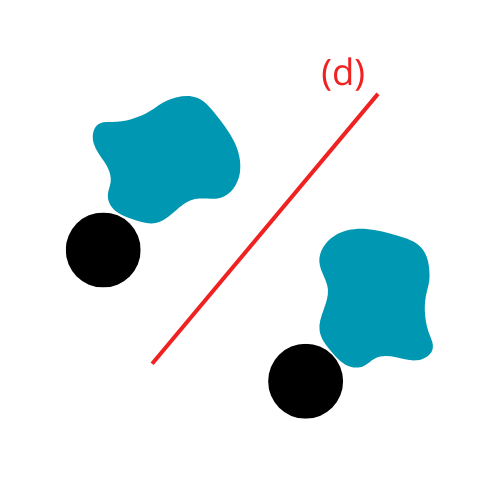
\includegraphics[width=0.70\linewidth]{symetrie_axiale.png}
    \caption{Symétrie axiale par rappot à la droite (d)}
    \label{fig:enter-label}
\end{figure}

\begin{tcolorbox}[colback=purple!10!white, colframe=pink!75!black, title=\textcolor{white}{Vocabulaire}, sharp corners=south]
    \begin{itemize}
        \item \textbf{Axe de symétrie} : Droite par rapport à laquelle la symétrie est effectuée.
        \item \textbf{Point symétrique} : Point obtenu par la symétrie d'un autre point par rapport à l'axe de symétrie.
        \item \textbf{Médiatrice} : Droite qui coupe un segment en son milieu et est perpendiculaire à ce segment.
    \end{itemize}
\end{tcolorbox}

\vspace{0.2cm}

\begin{tcolorbox}[colback=purple!10!white, colframe=purple!75!black, title=\textcolor{white}{Note}, sharp corners=south]
Deux figures symétriques ont les mêmes formes et dimensions.
\end{tcolorbox}

\vspace{0.35cm}

\subsubsection{\textcolor{green}{Les propriétés de la symétrie axiale}}

\vspace{0.3cm}

\begin{tcolorbox}[colback=blue!10!white, colframe=red!75!black, title=\textcolor{white}{Propriétés}, sharp corners=south]
    Voici les principales propriétés de la symétrie axiale :
    \begin{itemize}
        \item \textbf{Conservation des longueurs :} La symétrie axiale conserve la longueur des segments.
        \item \textbf{Conservation des angles :} Elle conserve aussi les mesures des angles.
        \item \textbf{Conservation des aires :} Les figures symétriques ont la même aire.
        \item \textbf{Conservation de l'alignement :} Si trois points sont alignés, leurs symétriques le sont aussi.
        \item \textbf{Symétrique d'une droite :} Le symétrique d'une droite par rapport à un axe est une droite.
        \item \textbf{Symétrique d'un cercle :} Le symétrique d'un cercle est un cercle de même rayon.
    \end{itemize}
\end{tcolorbox}

\vspace{0.3cm}

\begin{tcolorbox}[colback=orange!10!white, colframe=orange!75!black, title=\textcolor{white}{Exemple : Symétrie axiale d'un point}, sharp corners=south]
    Pour construire le symétrique d'un point \(A\) par rapport à une droite \(d\), il suffit de :
    \begin{enumerate}
        \item Tracer la perpendiculaire à la droite \(d\) passant par \(A\).
        \item Mesurer la distance entre \(A\) et \(d\), et reporter cette distance de l'autre côté de \(d\) pour obtenir le point \(A'\), symétrique de \(A\).
    \end{enumerate}
\end{tcolorbox}

\vspace{0.2cm}

Pour construire le symétrique d'une figure, on construit le symétrique de chacun des points qui la définissent et on reproduit la forme.

\begin{figure}[H]
    \centering
    \includegraphics[width=0.65\linewidth]{symétrique_figure.png}
    \caption{La construction du symétrique d'une figure}
    \label{fig:enter-label}
\end{figure}

\subsection{\textcolor{red}{Les axes de symétrie d'une figure}}

\subsubsection{\textcolor{green}{Symétrie d'une figure}}

\vspace{0.2cm}

\begin{tcolorbox}[colback=red!10!white, colframe=red!75!black, title=\textcolor{white}{Définition : Symétrie d'une figure}, sharp corners=south]
    Une figure possède un axe de symétrie si, lorsqu'on la plie le long de cet axe, ses deux parties se superposent exactement. La droite de symétrie est appelée \textit{axe de symétrie}. 
    La symétrie axiale est une transformation géométrique qui conserve les distances, les angles, les aires et les longueurs.
\end{tcolorbox}

\vspace{0.35cm}

Une figure peut avoir plusieurs axes de symétrie, comme un carré, qui en possède quatre (les deux axes diagonaux et les deux axes passant par les milieux de ses côtés opposés), ou bien aucun axe de symétrie, comme certaines figures irrégulières. 

\begin{itemize}
    \item **Cercle** : Le cercle possède une infinité d'axes de symétrie. Chaque diamètre constitue un axe de symétrie.
    \item **Triangle équilatéral** : Un triangle équilatéral possède trois axes de symétrie, chacun passant par un sommet et le milieu du côté opposé.
    \item **Rectangle (non carré)** : Un rectangle possède deux axes de symétrie, les deux axes passant par les milieux des côtés opposés.
    \item **Triangle scalène** : Un triangle scalène, sans côtés égaux, ne possède aucun axe de symétrie.
\end{itemize}

\vspace{0.35cm}

\begin{tcolorbox}[colback=red!10!white, colframe=blue!75!black, title=\textcolor{white}{Illustration : Figures avec et sans axes de symétrie}, sharp corners=south]
\begin{center}
    \begin{tikzpicture}
        % Dessin d'un carré avec 4 axes de symétrie
        \draw[thick] (-2,-2) rectangle (2,2);
        \draw[dashed, thick] (0,-2.5) -- (0,2.5); % Axe vertical
        \draw[dashed, thick] (-2.5,0) -- (2.5,0); % Axe horizontal
        \draw[dashed, thick] (-2.5,-2.5) -- (2.5,2.5); % Axe diagonal 1
        \draw[dashed, thick] (2.5,-2.5) -- (-2.5,2.5); % Axe diagonal 2
        \node at (0,-3) {Carré avec 4 axes de symétrie};

        % Décalage pour la deuxième figure
        \begin{scope}[shift={(7,0)}]
            % Dessin d'une forme irrégulière sans symétrie
            \draw[thick] (0,0) -- (1.5,1) -- (3,0.5) -- (2,-2) -- (0.5,-1.5) -- cycle;
            \node at (1,-3) {Figure irrégulière sans symétrie};
        \end{scope}
    \end{tikzpicture}
\end{center}
\end{tcolorbox}

\vspace{0.2cm}

\subsubsection{\textcolor{green}{Médiatrice d'un segment}}

\vspace{0.2cm}

\begin{tcolorbox}[colback=red!10!white, colframe=red!75!black, title=\textcolor{white}{Définition : }, sharp corners=south]
    \textbf{La médiatrice} d'un segment est la droite qui coupe ce segment en son milieu et qui est perpendiculaire à ce segment. Chaque point situé sur la médiatrice est équidistant des deux extrémités du segment. Elle est également l'axe de symétrie du segment.
\end{tcolorbox}

\vspace{0.2cm}

\begin{figure}[H]
    \centering
    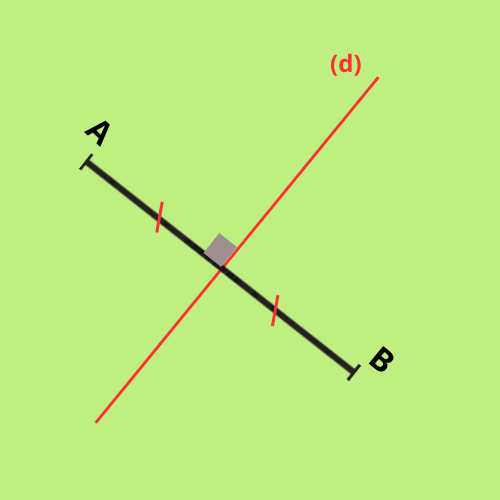
\includegraphics[width=0.47\linewidth]{segment_AB.png}
    \caption{La droite (d) et la médiatrice du segment[AB]}
    \label{fig:enter-label}
\end{figure}

\begin{tcolorbox}[colback=red!10!white, colframe=red!75!black, title=\textcolor{white}{Propriété }, sharp corners=south]
    La médiatrice d'un segment est l'axede symétrie de ce segment. Si (d) est la médiatrice du segment [AB], on dit que le point B est le symétrique du point A rapport à (d).
    Inversement, le symétrique du point A par rapport à une droite (d) est le point B tel que (d) soit la médiatrice du segment [AB]. SI le point A est sur la droite (d), son symétrique est lui-même: le point A est alors dit invariant. 
\end{tcolorbox}

\begin{tcolorbox}[colback=red!10!white, colframe=red!75!black, title=\textcolor{white}{Propriété}, sharp corners=south]
   Si un point est sur la médiatrice d'un segment, il est à égale distance des extrémités de ce segment.
\end{tcolorbox}

\begin{figure}[H]
    \centering
    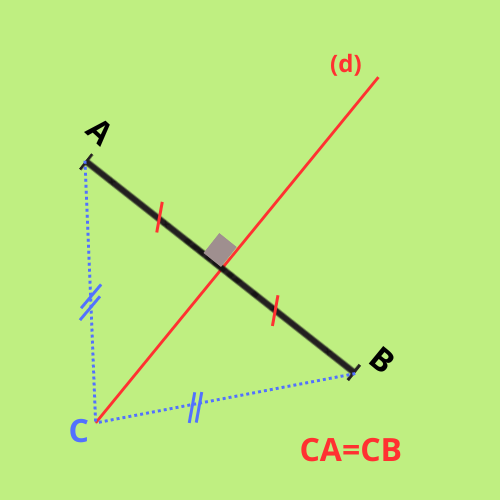
\includegraphics[width=0.47\linewidth]{egale_distance.png}
    \caption{Équidistance d'un point sur la Médiatrice d'un segment}
    \label{fig:enter-label}
\end{figure}

\begin{tcolorbox}[colback=red!10!white, colframe=red!75!black, title=\textcolor{white}{Propriété}, sharp corners=south]

Inversement, si un point est à égale distance des extrémités d'un segment, il appartient à la médiatrice de ce segment.
\end{tcolorbox}

\vspace{0.35cm}

\subsubsection{\textcolor{green}{Cerfs-volants}}

\vspace{0.2cm}

\begin{tcolorbox}[colback=red!10!white, colframe=red!75!black, title=\textcolor{white}{Définition : Cerf-volant}, sharp corners=south]
    Un cerf-volant est un quadrilatère dont une diagonale est un axe de symétrie.
\end{tcolorbox}

\vspace{0.2cm}

\begin{figure}[H]
    \centering
    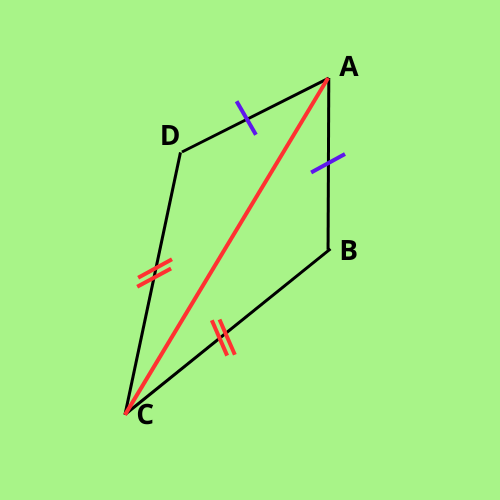
\includegraphics[width=0.5\linewidth]{cerf-volant.png}
    \caption{l'axe de symétrie dans le cerf-volant}
    \label{fig:enter-label}
\end{figure}

\vspace{0.2cm}

Le cerf-volant est un exemple de figure qui possède exactement un axe de symétrie. Les propriétés géométriques de cette figure sont importantes dans les études sur les quadrilatères particuliers.

\vspace{0.2cm}

\begin{tcolorbox}[colback=red!10!white, colframe=red!75!black, title=\textcolor{white}{Définition : Bissectrice}, sharp corners=south]
Dans un cerf-volant \( ABCD \) d'axe de symétrie \( (AC) \):
\begin{itemize}
    \item \( AB = AC \)
    \item \( CB = CD \)
    \item \( \widehat{ABC} = \widehat{ADC} \)
    \item \( AC \perp BD \)
\end{itemize}
\end{tcolorbox}

\subsubsection{\textcolor{green}{Bissectrice d'un angle}}

\vspace{0.2cm}

\begin{tcolorbox}[colback=red!10!white, colframe=red!75!black, title=\textcolor{white}{Définition : }, sharp corners=south]
    \textbf{La bissectrice} d'un angle est la demi-droite qui partage cet angle en deux angles de meme mesre. Chaque point de la bissectrice est équidistant des deux côtés de l'angle. Elle est aussi un axe de symétrie pour cet angle.
\end{tcolorbox}

\vspace{0.2cm}

\begin{figure}[H]
    \centering
    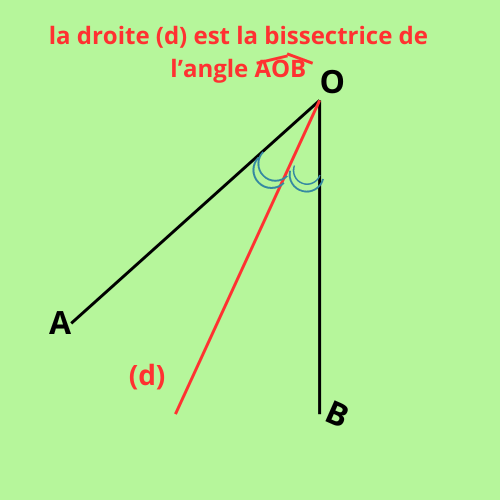
\includegraphics[width=0.5\linewidth]{bissectrice.png}
    \caption{Bissectrice d'un angle}
    \label{fig:enter-label}
\end{figure}

\vspace{0.2cm}

La bissectrice est une droite fondamentale dans la géométrie, notamment dans la construction des angles égaux et la résolution de problèmes géométriques impliquant la distance à des côtés d'un angle.

\vspace{0.2cm}

\begin{tcolorbox}[colback=blue!10!white, colframe=blue!75!black, title=\textcolor{white}{Récapitulatif }, sharp corners=south]
    \begin{itemize}
        \item La symétrie axiale consiste à superposer deux figures par rapport à une droite appelée \textbf{axe de symétrie}.
        \item Le \textbf{point symétrique} d’un point \( A \) par rapport à une droite \( d \) est obtenu en traçant une perpendiculaire à \( d \) depuis \( A \) et en mesurant la distance de \( A \) à \( d \).
        \item Les figures symétriques conservent leurs longueurs, angles et aires.
        \item Les axes de symétrie d’une figure peuvent varier. Par exemple :
            \begin{itemize}
                \item Un cercle a une infinité d'axes de symétrie.
                \item Un triangle équilatéral en a trois.
                \item Un rectangle a deux axes de symétrie.
                \item Un triangle scalène n’en a aucun.
            \end{itemize}
        \item La \textbf{médiatrice} d’un segment est la droite qui coupe ce segment en son milieu et est perpendiculaire à celui-ci. Chaque point sur la médiatrice est à la même distance des extrémités du segment.
    \end{itemize}
\end{tcolorbox}

\subsection{\textcolor{red}{Exercices et corrections}}

\vspace{0.2cm}

\begin{tcolorbox}[colback=yellow!10!white, colframe=yellow!75!black, title=\textcolor{white}{Exercices}, sharp corners=south]
    \begin{enumerate}
        \item \textbf{Exercice 1 :} Tracer le symétrique du point \( A(2, 3) \) par rapport à la droite \( d: y = 1 \). Donnez les coordonnées du point symétrique \( A' \).
        
        \item \textbf{Exercice 2 :} Considérez le triangle suivant avec les sommets \( A(1, 2) \), \( B(5, 6) \) et \( C(3, 8) \). Trouvez les coordonnées des points symétriques \( A' \), \( B' \) et \( C' \) par rapport à l'axe \( d: x = 4 \).

        \item \textbf{Exercice 3 :} Montrer que le rectangle \( R \) avec les sommets \( A(1, 1) \), \( B(1, 4) \), \( C(5, 4) \), et \( D(5, 1) \) a deux axes de symétrie. Indiquez ces axes.

        \item \textbf{Exercice 4 :} Donnez un exemple d'une figure qui n'a aucun axe de symétrie et expliquez pourquoi.

        \item \textbf{Exercice 5 :} Trouver la médiatrice du segment \( [PQ] \) avec \( P(-2, 1) \) et \( Q(4, 1) \). Quelle est la relation entre la médiatrice et les points \( P \) et \( Q \) ?

        \item \textbf{Exercice 6 :} Construisez le symétrique d'un cercle de centre \( O(3, 2) \) et de rayon 2 par rapport à une droite \( d: x = 5 \).

        \item \textbf{Exercice 7 :} Tracer un triangle isocèle dont un axe de symétrie est la droite \( d: x = 0 \). Indiquez les coordonnées des sommets du triangle et tracez son symétrique.

        \item \textbf{Exercice 8 :} Un trapèze \( ABCD \) a deux bases parallèles \( AB \) et \( CD \), avec \( AB = 2 \) cm, \( CD = 4 \) cm, et la hauteur \( h = 3 \) cm. Tracer le symétrique du trapèze par rapport à sa hauteur.

        \item \textbf{Exercice 9 :} Soit un hexagone régulier inscrit dans un cercle de centre \( O \) et de rayon 5 cm. Trouvez le nombre d'axes de symétrie de cet hexagone et expliquez votre démarche.

        \item \textbf{Exercice 10 :} Tracer un cerf-volant \( ABCD \) où \( AB = AC \) et \( BD \) est perpendiculaire à \( AC \). Indiquez l'axe de symétrie de la figure et vérifiez la propriété de la bissectrice.
        
        \item \textbf{Exercice 11 :} Soit le triangle équilatéral \( ABC \) avec \( AB = BC = CA = 4 \) cm. Trouvez les trois axes de symétrie du triangle, et vérifiez si le centre du cercle circonscrit au triangle coïncide avec le point d'intersection de ces axes.

        \item \textbf{Exercice 12 :} Dans un carré \( ABCD \), tracez ses deux diagonales \( AC \) et \( BD \). Montrez que ces diagonales sont des axes de symétrie du carré et vérifiez que \( AC \perp BD \). Trouvez également le point d'intersection des diagonales.

        \item \textbf{Exercice 13 :} Un losange \( ABCD \) a pour diagonales \( AC \) et \( BD \), qui se coupent perpendiculairement en leur milieu. Montrez que chaque diagonale est un axe de symétrie de la figure.
    \end{enumerate}
\end{tcolorbox}

\begin{tcolorbox}[colback=yellow!10!white, colframe=brown!75!black, title=\textcolor{white}{Pour allez plus loin}, sharp corners=south]

    \begin{enumerate}
        \item \textbf{Exercice 14 :} Tracez un rectangle dont les sommets sont \( A(0, 0) \), \( B(6, 0) \), \( C(6, 4) \), et \( D(0, 4) \). Trouvez les deux axes de symétrie du rectangle et vérifiez si l'intersection des diagonales est un point de symétrie.

        \item \textbf{Exercice 15 :} Soit un pentagone régulier inscrit dans un cercle de centre \( O \). Trouvez les axes de symétrie du pentagone et expliquez comment ils se relient à la symétrie axiale du cercle. Justifiez votre réponse en utilisant les propriétés de la médiatrice.
    \end{enumerate}
\end{tcolorbox}

\begin{tcolorbox}[colback=green!10!white, colframe=green!75!black, title=\textcolor{white}{Corrections des Exercices avec Graphiques}, sharp corners=south]

        \textbf{Exercice 1 :} Le symétrique du point \( A(2, 3) \) par rapport à la droite \( d : y = 1 \) :
        \begin{itemize}
            \item Le point symétrique \( A'(2, -1) \) est situé à une distance égale de la droite \( d \).
        \end{itemize}

        \begin{center}
        \begin{tikzpicture}[scale=1]
            % Axes
            \draw[->] (-1,0) -- (4,0) node[right] {$x$};
            \draw[->] (0,-3) -- (0,4) node[above] {$y$};
            
            % La droite d
            \draw[dashed, thick] (-1,1) -- (4,1) node[below right] {$d: y = 1$};

            % Points A et A'
            \filldraw[blue] (2,3) circle (2pt) node[right] {$A(2,3)$};
            \filldraw[red] (2,-1) circle (2pt) node[right] {$A'(2,-1)$};

            % Ligne de symétrie
            \draw[dashed] (2,3) -- (2,-1);
        \end{tikzpicture}
        \end{center}
        
        \textbf{Exercice 2 :} Symétrie des points \( A(1, 2) \), \( B(5, 6) \), \( C(3, 8) \) par rapport à l'axe \( x = 4 \) :
        \begin{itemize}
            \item \( A(1, 2) \rightarrow A'(7, 2) \)
            \item \( B(5, 6) \rightarrow B'(3, 6) \)
            \item \( C(3, 8) \rightarrow C'(5, 8) \)
        \end{itemize}

        \begin{center}
        \begin{tikzpicture}[scale=0.8]
            % Axes
            \draw[->] (-1,0) -- (8,0) node[right] {$x$};
            \draw[->] (0,-1) -- (0,9) node[above] {$y$};
            
            % La droite de symétrie
            \draw[dashed, thick] (4,-1) -- (4,9) node[above right] {$x = 4$};

            % Points A, B, C et leurs symétriques
            \filldraw[blue] (1,2) circle (2pt) node[below left] {$A(1,2)$};
            \filldraw[red] (7,2) circle (2pt) node[below right] {$A'(7,2)$};

            \filldraw[blue] (5,6) circle (2pt) node[above left] {$B(5,6)$};
            \filldraw[red] (3,6) circle (2pt) node[above left] {$B'(3,6)$};

            \filldraw[blue] (3,8) circle (2pt) node[above left] {$C(3,8)$};
            \filldraw[red] (5,8) circle (2pt) node[above right] {$C'(5,8)$};
        \end{tikzpicture}
        \end{center}
        
 
\end{tcolorbox}

\begin{tcolorbox}[colback=green!10!white, colframe=green!75!black, title=\textcolor{white}{Corrections des Exercices avec Graphiques}, sharp corners=south]

        \textbf{Exercice 3 :} Le rectangle \( R \) avec les sommets \( A(1, 1), B(1, 4), C(5, 4), D(5, 1) \) a deux axes de symétrie :
        \begin{itemize}
            \item L'axe vertical \( x = 3 \),
            \item L'axe horizontal \( y = 2.5 \).
        \end{itemize}

        \begin{center}
        \begin{tikzpicture}[scale=0.8]
            % Axes
            \draw[->] (-1,0) -- (6,0) node[right] {$x$};
            \draw[->] (0,-1) -- (0,5) node[above] {$y$};
            
            % Rectangle
            \draw[thick] (1,1) -- (1,4) -- (5,4) -- (5,1) -- cycle;

            % Sommets
            \filldraw[blue] (1,1) circle (2pt) node[below left] {$A(1,1)$};
            \filldraw[blue] (1,4) circle (2pt) node[above left] {$B(1,4)$};
            \filldraw[blue] (5,4) circle (2pt) node[above right] {$C(5,4)$};
            \filldraw[blue] (5,1) circle (2pt) node[below right] {$D(5,1)$};

            % Axes de symétrie
            \draw[dashed, thick] (3,-1) -- (3,5) node[above right] {$x = 3$};
            \draw[dashed, thick] (-1,2.5) -- (6,2.5) node[below right] {$y = 2.5$};
        \end{tikzpicture}
        \end{center}

        \textbf{Exercice 4 :} Un triangle scalène n'a pas d'axe de symétrie car ses côtés et ses angles sont tous différents.

\begin{center}
\begin{tikzpicture}[scale=0.8]
    % Axes
    \draw[->] (-1,0) -- (6,0) node[right] {$x$};
    \draw[->] (0,-1) -- (0,6) node[above] {$y$};
    
    % Triangle scalène
    \draw[thick] (1,1) -- (5,2) -- (3,4.5) -- cycle;

    % Sommets
    \filldraw[blue] (1,1) circle (2pt) node[below left] {$(1,1)$};
    \filldraw[blue] (5,2) circle (2pt) node[below right] {$(5,2)$};
    \filldraw[blue] (3,4.5) circle (2pt) node[above right] {$(3,4.5)$};
\end{tikzpicture}
\end{center}


        \textbf{Exercice 5 :} La médiatrice du segment \( [PQ] \) avec \( P(-2, 1) \) et \( Q(4, 1) \) est la droite \( x = 1 \).

        \begin{center}
        \begin{tikzpicture}[scale=0.8]
            % Axes
            \draw[->] (-3,0) -- (5,0) node[right] {$x$};
            \draw[->] (0,-1) -- (0,3) node[above] {$y$};
            
            % Segment PQ
            \draw[thick] (-2,1) -- (4,1);

            % Points P et Q
            \filldraw[blue] (-2,1) circle (2pt) node[below left] {$P(-2,1)$};
            \filldraw[blue] (4,1) circle (2pt) node[below right] {$Q(4,1)$};

            % Milieu du segment PQ
            \filldraw[red] (1,1) circle (2pt) node[above right] {$M(1,1)$};

            % Médiatrice
            \draw[dashed, thick] (1,-1) -- (1,3) node[above right] {$x = 1$};
        \end{tikzpicture}
        \end{center}

    La relation entre les points \( P \) et \( Q \) et leur médiatrice signifie que chaque point du segment \( [PQ] \) est à égale distance des deux points \( P \) et \( Q \), et la médiatrice est une droite perpendiculaire passant par le milieu de ce segment.

\end{tcolorbox}

\begin{tcolorbox}[colback=green!10!white, colframe=green!75!black, title=\textcolor{white}{Corrections des Exercices avec Graphiques}, sharp corners=south]

        \textbf{Exercice 6 :} Le cercle symétrique du cercle de centre \( O(3,2) \) et de rayon 2 par rapport à la droite \( d : x = 5 \) est le cercle de centre \( O'(7,2) \) et de rayon 2.

\begin{center}
\begin{tikzpicture}[scale=0.6]
    % Axes
    \draw[->] (-1,0) -- (10,0) node[right] {$x$};
    \draw[->] (0,-1) -- (0,6) node[above] {$y$};
    
    % La droite d : x = 5
    \draw[dashed, thick] (5,-1) -- (5,6) node[above right] {$x = 5$};
    
    % Cercle original de centre O(3,2) et de rayon 2
    \draw[thick, blue] (3,2) circle (2);
    \filldraw[blue] (3,2) circle (2pt) node[below left] {$O(3,2)$};
    
    % Cercle symétrique de centre O'(7,2) et de rayon 2
    \draw[thick, red] (7,2) circle (2);
    \filldraw[red] (7,2) circle (2pt) node[below right] {$O'(7,2)$};

    % Ligne de symétrie entre O et O'
    \draw[dashed] (3,2) -- (7,2);
\end{tikzpicture}
\end{center}



        \textbf{Exercice 7 :} Le triangle original a pour sommets \( A(-2,4) \), \( B(-1,1) \), \( C(-5,1) \) et son symétrique par rapport à la droite \( d : x = 0 \) a pour sommets \( A'(2,4) \), \( B'(1,1) \), et \( C'(5,1) \).


        \begin{center}
\begin{tikzpicture}[scale=0.8]
    % Axes
    \draw[->] (-6,0) -- (6,0) node[right] {$x$};
    \draw[->] (0,-1) -- (0,6) node[above] {$y$};

    % Axe de symétrie d
    \draw[dashed, thick] (0,-1) -- (0,6) node[above right] {$d : x = 0$};

    % Triangle original
    \filldraw[blue] (-3,4) circle (2pt) node[above left] {$A(-2,4)$};
    \filldraw[blue] (-1,1) circle (2pt) node[below right] {$B(-1,1)$};
    \filldraw[blue] (-5,1) circle (2pt) node[below left] {$C(-5,1)$};
    \draw[thick, blue] (-3,4) -- (-1,1) -- (-5,1) -- cycle;

    % Symétrique du triangle par rapport à d
    \filldraw[red] (3,4) circle (2pt) node[above right] {$A'(2,4)$};
    \filldraw[red] (1,1) circle (2pt) node[below right] {$B'(1,1)$};
    \filldraw[red] (5,1) circle (2pt) node[below right] {$C'(5,1)$};
    \draw[thick, red, dashed] (3,4) -- (1,1) -- (5,1) -- cycle;

    % Lignes reliant les sommets originaux et leurs symétriques
    \draw[dashed] (-3,4) -- (3,4);
    \draw[dashed] (-1,1) -- (1,1);
    \draw[dashed] (-5,1) -- (5,1);
\end{tikzpicture}
\end{center}

        \textbf{Exercice 8 :} Soit un trapèze \( ABCD \) avec les sommets \( A(-4,3) \), \( B(-2,3) \), \( C(-1,1) \), \( D(-5,1) \), où \( AB = 2 \) cm et \( CD = 4 \) cm. Le symétrique de ce trapèze par rapport à la hauteur passant par \( x = -1 \) est le trapèze \( A'B'C'D' \) avec les sommets \( A'(0,3) \), \( B'(2,3) \), \( C'(3,1) \), \( D'(-1,1) \).

\begin{center}
\begin{tikzpicture}[scale=0.8]
    % Axes
    \draw[->] (-6,0) -- (6,0) node[right] {$x$};
    \draw[->] (0,-1) -- (0,6) node[above] {$y$};

    % Axe de symétrie
    \draw[dashed, thick] (-1,-1) -- (-1,6) node[above right] {$\text{axe de symétrie } x = -1$};

    % Trapèze original
    \coordinate (A) at (-4,3); % Point A
    \coordinate (B) at (-2,3); % Point B
    \coordinate (C) at (-1,1); % Point C
    \coordinate (D) at (-5,1); % Point D

    % Trapèze original points and lines
    \filldraw[blue] (A) circle (2pt) node[above left=4pt] {$A(-4,3)$};
    \filldraw[blue] (B) circle (2pt) node[above right=4pt] {$B(-2,3)$};
    \filldraw[blue] (C) circle (2pt) node[below left=4pt] {$C(-1,1)$};
    \filldraw[blue] (D) circle (2pt) node[below left=4pt] {$D(-5,1)$};
    \draw[thick, blue] (A) -- (B) -- (C) -- (D) -- cycle;

    % Trapèze symétrique
    \coordinate (A') at (0,3); % Point A'
    \coordinate (B') at (2,3); % Point B'
    \coordinate (C') at (3,1); % Point C'
    \coordinate (D') at (-1,1); % Point D'

    % Trapèze symétrique points and lines
    \filldraw[red] (A') circle (2pt) node[above right=4pt] {$A'(0,3)$};
    \filldraw[red] (B') circle (2pt) node[above right=4pt] {$B'(2,3)$};
    \filldraw[red] (C') circle (2pt) node[below right=4pt] {$C'(3,1)$};
    \filldraw[red] (D') circle (2pt) node[below right=4pt] {$D'(-1,1)$};
    \draw[thick, red, dashed] (A') -- (B') -- (C') -- (D') -- cycle;

    % Lignes reliant les sommets originaux et leurs symétriques
    \draw[dashed] (A) -- (A');
    \draw[dashed] (B) -- (B');
    \draw[dashed] (C) -- (C');
    \draw[dashed] (D) -- (D');

    % Hauteur en vert
    \draw[thick, green] (-1,1) -- (-1,3) node[midway, left=5pt] {$h = 3 \, \text{cm}$};

\end{tikzpicture}
\end{center}
\end{tcolorbox}

\begin{tcolorbox}[colback=green!10!white, colframe=green!75!black, title=\textcolor{white}{Corrections des Exercices avec Graphiques}, sharp corners=south]

        \textbf{Exercice 9 :} Soit un hexagone régulier inscrit dans un cercle de centre \( O \) et de rayon 5 cm.

        \begin{figure}[H]
            \centering
            \includegraphics[width=0.3\linewidth]{axes de symétries.png}
            \caption{L'hexagone régulier inscrit dans un cercle}
            \label{fig:enter-label}
        \end{figure}

        Un hexagone régulier inscrit dans un cercle a 6 axes de symétrie, comprenant 3 axes passant par les sommets et 3 axes passant par les milieux des côtés. Chaque axe de symétrie divise l'hexagone en deux parties égales et superposables. Par conséquent, un hexagone régulier a un total de 6 axes de symétrie.

        \vspace{0.3cm}

       \begin{multicols}{2} % Crée une colonne pour le texte et une pour le schéma

\textbf{Exercice 10 :} Dans un cerf-volant \( ABCD \) d'axe de symétrie \( (BD) \):
\begin{itemize}
    \item \( AB = BC \)
    \item \( AD = CD \)
    \item \( \widehat{BAD} = \widehat{BCD} \)
    \item \( AC \perp BD \)
\end{itemize}

\columnbreak % Passe à la colonne suivante pour le schéma

\begin{center}
\begin{tikzpicture}[scale=0.6]
    % Axes
    \draw[->] (-2,0) -- (6,0) node[right] {$x$};
    \draw[->] (0,-2) -- (0,6) node[above] {$y$};
    
    % Cerf-volant ABCD
    \draw[thick] (1,2) -- (3,4) -- (5,2) -- (3,-1) -- cycle;

    % Sommets
    \filldraw[blue] (1,2) circle (2pt) node[below left] {$A(1,2)$};
    \filldraw[blue] (3,4) circle (2pt) node[above left] {$B(3,4)$};
    \filldraw[blue] (5,2) circle (2pt) node[above right] {$C(5,2)$};
    \filldraw[blue] (3,-1) circle (2pt) node[below right] {$D(3,-1)$};

    % Axes de symétrie
    \draw[dashed, thick] (1,2) -- (5,2) node[above left] {$y = 2$};
    \draw[dashed, thick] (3,4) -- (3,-1) node[above left] {$x = 3$};
\end{tikzpicture}
\end{center}

\end{multicols}

    \textbf{Exercice 11 :} Le triangle \( ABC \) a pour sommets \( A(1, 1) \), \( B(5, 1) \), \( C(3, 4.5) \). Son centre de gravité \( G \) est donné par les coordonnées 
    \[
    G\left( \frac{1+5+3}{3}, \frac{1+1+4.5}{3} \right) = G(3, \frac{13}{6}) \simeq G(3, 2.16).
    \]

    \begin{center}
    \begin{tikzpicture}[scale=0.6]
        % Axes
        \draw[->] (-1,0) -- (6,0) node[right] {$x$};
        \draw[->] (0,-1) -- (0,6) node[above] {$y$};
        
        % Triangle
        \draw[thick] (1,1) -- (5,1) -- (3,4.5) -- cycle;

        % Sommets
        \filldraw[blue] (1,1) circle (2pt) node[below left] {$(1,1)$};
        \filldraw[blue] (5,1) circle (2pt) node[below right] {$(5,1)$};
        \filldraw[blue] (3,4.5) circle (2pt) node[above right] {$(3,4.5)$};
        \filldraw[red] (3,2.16) circle (2pt) node[above right] {$G(3,2.16)$};

        % Cercle circonscrit
        \draw[red, thick] (3, 2.16) circle (2.5); % Cercle circonscrit

        % Axes de symétrie
        \draw[blue, dashed] (3,0) -- (3,5); % Axe vertical passant par G
        \draw[blue, dashed] (1,1) -- (6,4); % Axe de symétrie passant par A et C
        \draw[blue, dashed] (5,1) -- (0,4); % Axe de symétrie passant par B et C
    \end{tikzpicture}
    \end{center}

\end{tcolorbox}


\begin{tcolorbox}[colback=green!10!white, colframe=green!75!black, title=\textcolor{white}{Corrections des Exercices avec Graphiques}, sharp corners=south]

        \textbf{Exercice 12 :} \textbf{Axes de symétrie :} Dans un carré \(ABCD\), les diagonales \( AC \) et \( BD \) divisent la figure en deux parties identiques. Ainsi, chaque diagonale est un axe de symétrie du carré. Toute rotation de \( 180^\circ \) autour du point \( O \) ou toute réflexion le long de l’une des diagonales laisse le carré inchangé.

        \vspace{0.2cm}

       \textbf{Perpendicularité des diagonales :} Les diagonales \( AC \) et \( BD \) sont perpendiculaires. Comme le carré est une figure régulière avec des angles droits, ses diagonales se croisent toujours à angle droit.


\begin{center}
\begin{tikzpicture}[scale=1.5]
    % Carré ABCD
    \coordinate (A) at (0,0);
    \coordinate (B) at (2,0);
    \coordinate (C) at (2,2);
    \coordinate (D) at (0,2);
    
    % Tracé du carré
    \draw[thick] (A) -- (B) -- (C) -- (D) -- cycle;
    
    % Etiquettes des sommets
    \node[below left] at (A) {\( A \)};
    \node[below right] at (B) {\( B \)};
    \node[above right] at (C) {\( C \)};
    \node[above left] at (D) {\( D \)};
    
    % Tracé des diagonales
    \draw[dashed, blue] (A) -- (C);
    \draw[dashed, blue] (B) -- (D);
    
    % Point d'intersection des diagonales
    \coordinate (O) at (intersection of A--C and B--D);
    \filldraw[red] (O) circle (1.5pt) node[below right] {\( O \)};

\end{tikzpicture}
\end{center}

\textbf{Point d'intersection :} Les diagonales se croisent au centre du carré, que nous notons \( O \). Ce point \( O \) est aussi le centre du cercle circonscrit au carré et se situe à égale distance des sommets \( A \), \( B \), \( C \), et \( D \).

\vspace{0.3cm}

        \textbf{Exercice 13 :} Pour démontrer que chaque diagonale est un axe de symétrie du losange \( ABCD \), considérons ses diagonales \( AC \) et \( BD \), qui se coupent perpendiculairement en leur milieu \( O \). Chacune d'elles divise le losange en deux triangles superposables : \( AC \) sépare le triangle \( ABC \) et le triangle \( ADC \), tandis que \( BD \) sépare le triangle \( ABD \) et le triangle \( CBD \). Ainsi, \( AC \) et \( BD \) sont des axes de symétrie du losange, et leur intersection perpendiculaire au point \( O \) confirme cette propriété de symétrie.

\begin{center}
\begin{tikzpicture}[scale=1.5]
    % Losange ABCD
    \coordinate (A) at (0,1.5);
    \coordinate (B) at (2,0);
    \coordinate (C) at (0,-1.5);
    \coordinate (D) at (-2,0);
    
    % Tracé du losange
    \draw[thick] (A) -- (B) -- (C) -- (D) -- cycle;
    
    % Etiquettes des sommets
    \node[above] at (A) {\( A \)};
    \node[right] at (B) {\( B \)};
    \node[below] at (C) {\( C \)};
    \node[left] at (D) {\( D \)};
    
    % Tracé des diagonales
    \draw[dashed, blue] (A) -- (C);
    \draw[dashed, blue] (B) -- (D);
    
    % Point d'intersection des diagonales
    \coordinate (O) at (intersection of A--C and B--D);
    \filldraw[red] (O) circle (1.5pt) node[below right] {\( O \)};
    
    % Marque l'angle droit entre les diagonales
    \draw[red] (O) ++(0.15,0) -- ++(0,0.15) -- ++(-0.15,0);
\end{tikzpicture}
\end{center}
\end{tcolorbox}

\newpage
\section{\textcolor{blue}{Chapitre 6: Programmation}}

La programmation est un moyen de donner des instructions à un ordinateur pour qu'il exécute des tâches spécifiques. C'est un peu comme un chef qui suit une recette pour préparer un plat. Dans cette section, nous allons découvrir ce qu'est un algorithme, explorer les différentes manières de déplacer des objets à l'écran, et enfin, nous allons écrire notre premier algorithme.

\subsection{\textcolor{red}{Algorithme}}

Un algorithme est une suite d'étapes à suivre pour résoudre un problème ou accomplir une tâche. Pense à un algorithme comme une recette de cuisine : il te dit quoi faire, dans quel ordre et avec quels ingrédients. Par exemple, pour préparer un gâteau, tu as besoin d'une liste d'ingrédients et d'étapes précises à suivre.

\subsubsection{\textcolor{green}{Définitions et Algorithmes élémentaires}}

Pour bien comprendre ce qu'est un algorithme, voici quelques définitions importantes :

\begin{tcolorbox}[colback=red!10!white, colframe=red!75!black, title=\textcolor{white}{Définitions}]
\begin{itemize}
    \item \textbf{Instruction} : C'est une action que l'ordinateur doit réaliser. Par exemple, additionner deux nombres ou afficher un message à l'écran.
    \item \textbf{Entrée} : Ce sont les données que l'utilisateur fournit à l'algorithme. Par exemple, les deux nombres que tu veux additionner ou le nombre dont tu veux afficher la table de multiplication.
    \item \textbf{Sortie} : C'est le résultat que l'algorithme produit après avoir traité les entrées. Par exemple, la somme de ces deux nombres ou les résultats de la multiplication.
\end{itemize}
\end{tcolorbox}

Pour illustrer ces concepts, regardons un exemple d'un algorithme simple pour additionner deux nombres :

\begin{tcolorbox}[colback=orange!10!white, colframe=orange!75!black, title=\textcolor{white}{Exemple d'Addition}]
\begin{algorithm}[H]
\caption{Addition de deux nombres}
\begin{algorithmic}[1]
\State \textbf{Entrée} : Deux nombres \( a \) et \( b \)
\State \( S \gets a + b \)
\State \textbf{Sortie} : \( S \)
\end{algorithmic}
\end{algorithm}
Cet algorithme dit d'abord de prendre deux nombres, puis d'additionner ces deux nombres, et enfin de donner le résultat.
\end{tcolorbox}

Cet exemple montre comment un algorithme fonctionne : il prend des entrées, effectue des calculs, puis donne une sortie.


\begin{tcolorbox}[colback=orange!10!white, colframe=orange!75!black, title=\textcolor{white}{Exemple de Multiplication}]
\begin{algorithm}[H]
\caption{Multiplication de deux nombres}
\begin{algorithmic}[1]
\State \textbf{Entrée} : Deux nombres \( a \) et \( b \)
\State \textbf{Initialisation} : \( P \gets 0 \)
\State \textbf{ Pour \( i \) allant de \(1 \) à \( b \)} \textbf{faire}  
    \State \( P \gets P + a \)
\State \textbf{Fin pour}
\State \textbf{Sortie} : \( P \)
\end{algorithmic}
\end{algorithm}
\end{tcolorbox}

Cet algorithme commence par initialiser le produit \( P \) à 0, puis utilise une boucle pour additionner \( a \) à lui-même \( b \) fois, produisant ainsi le produit \( P \).

\vspace{0.15cm}

Dans la programmation, il est souvent nécessaire de déplacer un objet à l'écran. Ces déplacements peuvent être :

\begin{tcolorbox}[colback=red!10!white, colframe=red!75!black, title=\textcolor{white}{Définitions}]
\begin{itemize}
    \item \textbf{Déplacements absolus} : Cela signifie que tu dis exactement où aller. Par exemple, "Va à la position \( (5, 3) \)" signifie que l'objet doit se rendre exactement à cette position sur l'écran.
    \item \textbf{Déplacements relatifs} : Cela signifie que tu dis combien tu veux bouger par rapport à ta position actuelle. Par exemple, "Déplace-toi de 3 vers la droite" signifie que tu commences à partir de ta position actuelle et que tu te déplaces vers la droite.
\end{itemize}
\end{tcolorbox}

Pour mieux comprendre, imagine que tu joues à un jeu vidéo. Si tu veux que ton personnage se déplace à un endroit précis sur la carte, tu utiliserais un déplacement absolu. En revanche, si tu veux que ton personnage avance de quelques pas par rapport à sa position actuelle, tu utiliserais un déplacement relatif.

\subsubsection{\textcolor{green}{Mon premier Algorithme}}

Écrivons ensemble notre premier algorithme ! Imaginons que nous voulons calculer la table de multiplication d'une variable quelconque \( a \). Voici comment cela se présente :

\begin{tcolorbox}[colback=brown!10!white, colframe=brown!75!black, title=\textcolor{white}{Mon premier Algorithme}]

\begin{algorithm}[H]
    \caption{Calcul de la table de multiplication de \( a \)}
    \begin{algorithmic}[1]
        \State \textbf{Entrée} : Nombre \( a \)
        \State \textbf{Initialisation} : \( i \gets 1 \)
        \State \textbf{tant que}  \( i \leq 10 \) \textbf{faire} 
            \State Résultat \( \gets a \times i \)
            \State Afficher \( a \times i = \text{Résultat} \)
            \State \( i \gets i + 1 \)
        \State Fin tant que
        \State \textbf{Sortie} : Les résultats affichés
    \end{algorithmic}
\end{algorithm}
\end{tcolorbox}

Cet algorithme commence par demander à l'utilisateur de saisir un nombre \( a \), initialise une variable \( i \) à 1, puis utilise une boucle pour multiplier \( a \) par \( i \) et afficher les résultats de la multiplication de 1 à 10.


\begin{tcolorbox}[colback=cyan!10!white, colframe=cyan!75!black, title=\textcolor{white}{Récapitulatif}]
Dans cette section, nous avons appris que :
\begin{itemize}
    \item Un algorithme est une suite d'étapes pour accomplir une tâche, similaire à une recette.
    \item Les instructions, entrées et sorties sont des éléments clés d'un algorithme.
    \item Les déplacements peuvent être absolus (position exacte) ou relatifs (par rapport à la position actuelle).
    \item Nous avons écrit notre premier algorithme pour calculer la table de multiplication d'une variable \( a \).
    \item Nous avons également vu un algorithme pour multiplier deux nombres.
\end{itemize}
\end{tcolorbox}

\subsection{\textcolor{red}{Exercices et Corrections}}

\begin{tcolorbox}[colback=green!10!white, colframe=yellow!75!black, title=\textcolor{white}{Exercices}]

\textbf{Exercice 1 : Compréhension d'un algorithme simple}

\textbf{Énoncé :} \\
Écris un algorithme qui prend deux nombres comme entrée et affiche leur différence.

\textbf{Consignes :}
\begin{itemize}
    \item L'algorithme doit demander à l'utilisateur deux nombres \( x \) et \( y \).
    \item Il doit calculer la différence \( D = x - y \).
    \item L'algorithme doit afficher \( D \).
\end{itemize}

\textbf{Exemple :}
\begin{verbatim}
Entrée : 10 et 5
Sortie : 5
\end{verbatim}

\vspace{0.5cm}

\textbf{Exercice 2 : Déplacement relatif}

\textbf{Énoncé :} \\
Supposons que tu sois en train de programmer un robot qui se déplace sur une grille en 2D. Écris un algorithme qui déplace le robot de manière relative.

\textbf{Consignes :}
\begin{itemize}
    \item Le robot commence à la position \( (0, 0) \).
    \item À chaque étape, donne une direction de déplacement (Haut, Bas, Gauche, Droite) et de combien de cases il doit bouger.
    \item L'algorithme doit afficher la nouvelle position après chaque déplacement.
\end{itemize}

\textbf{Exemple :}
\begin{verbatim}
Position initiale : (0, 0)
Déplacement : Haut de 2
Nouvelle position : (0, 2)
Déplacement : Droite de 3
Nouvelle position : (3, 2)
\end{verbatim}

\vspace{0.5cm}

\textbf{Exercice 3 : Calcul de la somme des \( n \) premiers nombres}

\textbf{Énoncé :} \\
Écris un algorithme qui calcule et affiche la somme des \( n \) premiers nombres entiers, où \( n \) est fourni par l'utilisateur.

\textbf{Consignes :}
\begin{itemize}
    \item L'algorithme doit demander à l'utilisateur un nombre \( n \).
    \item Il doit utiliser une boucle pour calculer la somme des entiers de 1 à \( n \).
    \item L'algorithme doit afficher la somme totale.
\end{itemize}

\textbf{Exemple :}
\begin{verbatim}
Entrée : 5
Sortie : 15 (car 1 + 2 + 3 + 4 + 5 = 15)
\end{verbatim}

\end{tcolorbox}

\begin{tcolorbox}[colback=green!10!white, colframe=yellow!75!black, title=\textcolor{white}{Exercices}]

\textbf{Exercice 4 : Algorithme de déplacement absolu}

\textbf{Énoncé :} \\
Écris un algorithme qui déplace un point à une position absolue sur une grille.

\textbf{Consignes :}
\begin{itemize}
    \item L'utilisateur donne les coordonnées \( x \) et \( y \) où il souhaite déplacer le point.
    \item L'algorithme doit afficher la nouvelle position.
\end{itemize}

\textbf{Exemple :}
\begin{verbatim}
Entrée : 4 et 7
Sortie : Position : (4, 7)
\end{verbatim}

\vspace{0.5cm}

\textbf{Exercice 5 : Algorithme de multiplication sans utiliser l'opérateur \(*\)}

\textbf{Énoncé :} \\
Écris un algorithme qui calcule le produit de deux nombres sans utiliser directement l'opérateur de multiplication (\(*\)).

\textbf{Consignes :}
\begin{itemize}
    \item L'algorithme doit demander à l'utilisateur deux nombres \( a \) et \( b \).
    \item Il doit utiliser une boucle pour additionner \( a \) à lui-même \( b \) fois.
    \item L'algorithme doit afficher le produit \( a \times b \).
\end{itemize}

\textbf{Exemple :}
\begin{verbatim}
Entrée : 4 et 3
Sortie : 12 (car 4 + 4 + 4 = 12)
\end{verbatim}

\vspace{0.5cm}

\textbf{Exercice 6 : Table de multiplication}

\textbf{Énoncé :} \\
Modifie l'algorithme pour calculer la table de multiplication d'un nombre, mais cette fois-ci, l'algorithme doit demander à l'utilisateur le nombre maximum pour lequel la table de multiplication doit être calculée.

\textbf{Consignes :}
\begin{itemize}
    \item L'utilisateur entre le nombre \( a \) pour lequel il veut calculer la table de multiplication et un nombre maximum \( n \).
    \item L'algorithme affiche la table de multiplication de \( a \) jusqu'à \( a \times n \).
\end{itemize}

\textbf{Exemple :}
\begin{verbatim}
Entrée : 3 et 5
Sortie :
3 x 1 = 3
3 x 2 = 6
3 x 3 = 9
3 x 4 = 12
3 x 5 = 15
\end{verbatim}
\end{tcolorbox}

\begin{tcolorbox}[colback=green!10!white, colframe=yellow!75!black, title=\textcolor{white}{Exercices}]

\textbf{Exercice 7 : Trouver le plus grand de trois nombres}

\textbf{Énoncé :} \\
Écris un algorithme qui trouve et affiche le plus grand de trois nombres.

\textbf{Consignes :}
\begin{itemize}
    \item L'algorithme doit demander à l'utilisateur trois nombres \( a \), \( b \), et \( c \).
    \item Il doit comparer les trois et afficher le plus grand.
\end{itemize}

\textbf{Exemple :}
\begin{verbatim}
Entrée : 12, 7 et 9
Sortie : Le plus grand est 12
\end{verbatim}

\vspace{0.5cm}

\textbf{Exercice 8 : Compteur de boucles}

\textbf{Énoncé :} \\
Écris un algorithme qui demande à l'utilisateur un nombre \( n \) et utilise une boucle pour afficher un message \( n \) fois.

\textbf{Consignes :}
\begin{itemize}
    \item L'algorithme demande à l'utilisateur un nombre \( n \).
    \item Il doit afficher "Ceci est la boucle numéro \( i \)" pour chaque itération de 1 à \( n \).
\end{itemize}

\textbf{Exemple :}
\begin{verbatim}
Entrée : 3
Sortie :
Ceci est la boucle numéro 1
Ceci est la boucle numéro 2
Ceci est la boucle numéro 3
\end{verbatim}
\end{tcolorbox}

\vspace{0.2cm}

\begin{tcolorbox}[colback=green!10!white, colframe=green!75!black, title=\textcolor{white}{  Corrections}]

\textbf{Exercice 1 : Compréhension d'un algorithme simple}

\textbf{Correction :} \\
L'algorithme demande deux nombres à l'utilisateur et affiche leur différence.

\begin{verbatim}
Début
   Lire x, y
   D = x - y
   Afficher D
Fin
\end{verbatim}

Exemple d'exécution :
\begin{verbatim}
Entrée : 10 et 5
Sortie : 5
\end{verbatim}

\end{tcolorbox}

\begin{tcolorbox}[colback=green!10!white, colframe=green!75!black, title=\textcolor{white}{  Corrections}]

\textbf{Exercice 2 : Déplacement relatif}

\textbf{Correction :} \\
Le robot se déplace sur une grille à partir de la position \( (0, 0) \). Après chaque déplacement, sa position est mise à jour et affichée.

\begin{verbatim}
Début
   Position = (0, 0)
   Tant que l'utilisateur veut se déplacer faire
      Lire direction, nb_cases
      Si direction = "Haut" alors
         Position.y = Position.y + nb_cases
      Sinon si direction = "Bas" alors
         Position.y = Position.y - nb_cases
      Sinon si direction = "Gauche" alors
         Position.x = Position.x - nb_cases
      Sinon si direction = "Droite" alors
         Position.x = Position.x + nb_cases
      Fin Si
      Afficher Position
   Fin Tant que
Fin
\end{verbatim}

Exemple d'exécution :
\begin{verbatim}
Position initiale : (0, 0)
Déplacement : Haut de 2
Nouvelle position : (0, 2)
Déplacement : Droite de 3
Nouvelle position : (3, 2)
\end{verbatim}

\vspace{0.5cm}

\textbf{Exercice 3 : Calcul de la somme des \( n \) premiers nombres}

\textbf{Correction :} \\
L'algorithme calcule la somme des \( n \) premiers nombres entiers.

\begin{verbatim}
Début
   Lire n
   Somme = 0
   Pour i allant de 1 à n faire
      Somme = Somme + i
   Fin Pour
   Afficher Somme
Fin
\end{verbatim}

Exemple d'exécution :
\begin{verbatim}
Entrée : 5
Sortie : 15
\end{verbatim}

\end{tcolorbox}

\begin{tcolorbox}[colback=green!10!white, colframe=green!75!black, title=\textcolor{white}{  Corrections}]

\textbf{Exercice 4 : Algorithme de déplacement absolu}

\textbf{Correction :} \\
L'algorithme demande les coordonnées \( x \) et \( y \) et affiche la position absolue.

\begin{verbatim}
Début
   Lire x, y
   Afficher "Position : (", x, ",", y, ")"
Fin
\end{verbatim}

Exemple d'exécution :
\begin{verbatim}
Entrée : 4 et 7
Sortie : Position : (4, 7)
\end{verbatim}

\vspace{0.5cm}

\textbf{Exercice 5 : Algorithme de multiplication sans utiliser l'opérateur \(*\)}

\textbf{Correction :} \\
L'algorithme utilise une boucle pour additionner un nombre à lui-même plusieurs fois, correspondant au produit des deux nombres.

\begin{verbatim}
Début
   Lire a, b
   Produit = 0
   Pour i allant de 1 à b faire
      Produit = Produit + a
   Fin Pour
   Afficher Produit
Fin
\end{verbatim}

Exemple d'exécution :
\begin{verbatim}
Entrée : 4 et 3
Sortie : 12
\end{verbatim}

\vspace{0.5cm}

\textbf{Exercice 6 : Table de multiplication}

\textbf{Correction :} \\
L'algorithme calcule la table de multiplication jusqu'à \( n \) pour un nombre donné.

\begin{verbatim}
Début
   Lire a, n
   Pour i allant de 1 à n faire
      Afficher a, " x ", i, " = ", a * i
   Fin Pour
Fin
\end{verbatim}

Exemple d'exécution :
\begin{verbatim}
Entrée : 3 et 5
Sortie :
3 x 1 = 3
3 x 2 = 6
3 x 3 = 9
3 x 4 = 12
3 x 5 = 15
\end{verbatim}

\end{tcolorbox}

\begin{tcolorbox}[colback=green!10!white, colframe=green!75!black, title=\textcolor{white}{  Corrections}]

\textbf{Exercice 7 : Trouver le plus grand de trois nombres}

\textbf{Correction :} \\
L'algorithme compare trois nombres et affiche le plus grand.

\begin{verbatim}
Début
   Lire a, b, c
   Si a > b et a > c alors
      Afficher a
   Sinon si b > a et b > c alors
      Afficher b
   Sinon
      Afficher c
   Fin Si
Fin
\end{verbatim}

Exemple d'exécution :
\begin{verbatim}
Entrée : 12, 7 et 9
Sortie : Le plus grand est 12
\end{verbatim}

\vspace{0.5cm}

\textbf{Exercice 8 : Compteur de boucles}

\textbf{Correction :} \\
L'algorithme utilise une boucle pour afficher un message un nombre spécifique de fois.

\begin{verbatim}
Début
   Lire n
   Pour i allant de 1 à n faire
      Afficher "Ceci est la boucle numéro ", i
   Fin Pour
Fin
\end{verbatim}

Exemple d'exécution :
\begin{verbatim}
Entrée : 3
Sortie :
Ceci est la boucle numéro 1
Ceci est la boucle numéro 2
Ceci est la boucle numéro 3
\end{verbatim}
\end{tcolorbox}

\newpage
\section{\textcolor{blue}{Chapitre 7: Statistiques}}

\subsection{\textcolor{red}{Définitions (Effectifs et Fréquences)}}

Les statistiques nous aident à organiser et analyser des données. Cela peut être utile pour mieux comprendre des informations comme des résultats d'examen, des enquêtes, ou même des préférences personnelles. Pour commencer, deux notions essentielles en statistiques sont l'effectif et la fréquence. 

Voyons ensemble ce que ces termes signifient.

\subsubsection{\textcolor{green}{Tableaux d'effectifs}}

\tcbset{colback=red!10!white, colframe=red!75!black, title=\textcolor{white}{Définition}}
\begin{tcolorbox}
\textbf{ L'effectif} d'une donnée est le nombre de fois où cette donnée apparaît dans un ensemble. Il représente donc une quantité ou une occurrence. En d'autres termes, c'est le nombre total d'éléments que l'on peut compter pour une catégorie donnée.
\end{tcolorbox}

\tcbset{colback=orange!10!white, colframe=orange!75!black, title=\textcolor{white}{Exemple}}
\begin{tcolorbox}
\textbf{Exemple :} \\  
Imaginons que tu fasses un sondage dans ta classe pour connaître le nombre d'élèves qui possèdent un animal de compagnie. Voici ce que tu trouves :
\begin{itemize}
    \item 5 élèves ont un chien.
    \item 3 élèves ont un chat.
    \item 2 élèves ont un poisson.
\end{itemize}
Le tableau d'effectifs se présente ainsi :

\begin{center}
\begin{tabular}{|c|c|}
\hline
Animal & Effectif \\
\hline
Chien & 5 \\
Chat & 3 \\
Poisson & 2 \\
\hline
\end{tabular}
\end{center}

Ici, l'effectif pour chaque animal correspond au nombre d'élèves ayant cet animal comme compagnon.
\end{tcolorbox}

\subsubsection{\textcolor{green}{Tableaux de fréquences}}

Maintenant que nous comprenons l'effectif, passons à la fréquence.

\tcbset{colback=red!10!white, colframe=red!75!black, title=\textcolor{white}{Définition}}
\begin{tcolorbox}
\textbf{La fréquence} indique la proportion ou le pourcentage d'une catégorie par rapport à l'ensemble des données. Elle se calcule en divisant l'effectif d'une catégorie par le nombre total d'éléments. La fréquence nous donne une idée de la part que représente chaque catégorie.
\end{tcolorbox}

\vspace{0.15cm}

\tcbset{colback=purple!10!white, colframe=purple!75!black, title=\textcolor{white}{Note pédagogique}}
\begin{tcolorbox}
\textbf{Note :} \\
L'effectif donne le nombre exact de données pour une catégorie, tandis que la fréquence indique sa proportion dans le total. La somme des fréquences doit toujours être égale à 1 (ou 100\% si on parle en pourcentage).
\end{tcolorbox}

\tcbset{colback=orange!10!white, colframe=orange!75!black, title=\textcolor{white}{Exemple}}
\begin{tcolorbox}
\textbf{Exemple :} \\  
Reprenons l'exemple des animaux. Il y a 10 élèves au total dans la classe (5 ont un chien, 3 ont un chat, 2 ont un poisson). La fréquence de chaque animal est calculée ainsi :

\begin{itemize}
    \item Fréquence des élèves ayant un chien : \( \frac{5}{10} = 0,5 \), soit 50\%.
    \item Fréquence des élèves ayant un chat : \( \frac{3}{10} = 0,3 \), soit 30\%.
    \item Fréquence des élèves ayant un poisson : \( \frac{2}{10} = 0,2 \), soit 20\%.
\end{itemize}

Le tableau de fréquences se présente ainsi :

\begin{center}
\begin{tabular}{|c|c|}
\hline
Animal & Fréquence \\
\hline
Chien & 50\% \\
Chat & 30\% \\
Poisson & 20\% \\
\hline
\end{tabular}
\end{center}

Les fréquences nous aident à mieux comprendre la répartition des animaux dans la classe. Par exemple, 50\% des élèves ont un chien, ce qui signifie que la moitié des élèves possèdent un chien.
\end{tcolorbox}

\tcbset{colback=purple!10!white, colframe=purple!75!black, title=\textcolor{white}{Note pédagogique}}
\begin{tcolorbox}
\textbf{Astuce :} \\
Lorsque tu calcules une fréquence, il suffit de diviser l'effectif par le nombre total de données. Ensuite, tu peux multiplier le résultat par 100 pour obtenir un pourcentage. Par exemple, pour calculer la fréquence en pourcentage d'une catégorie avec un effectif de 4 sur 20 éléments au total, tu fais \( \frac{4}{20} \times 100 = 20\% \).
\end{tcolorbox}

\vspace{0.15cm}

\tcbset{colback=cyan!10!white, colframe=cyan!75!black, title=\textcolor{white}{Récapitulatif}}
\begin{tcolorbox}
\textbf{Ce qu'il faut retenir :}
\begin{itemize}
    \item L'effectif est le nombre de fois où une donnée apparaît dans un ensemble.
    \item La fréquence est la proportion de cette donnée par rapport au total des données.
    \item Les tableaux d'effectifs et de fréquences nous aident à organiser et comprendre les données.
    \item La somme des fréquences doit toujours être égale à 1 ou 100\%.
\end{itemize}
\end{tcolorbox}

\subsection{\textcolor{red}{Exercices et Corrections}}

\begin{tcolorbox}[colback=green!10!white, colframe=yellow!75!black, title=\textcolor{white}{Exercices}]

\textbf{Exercice 1 : Calculer l'effectif}

Un professeur demande à ses élèves leur fruit préféré. Voici les réponses obtenues :
\begin{itemize}
    \item 6 élèves préfèrent la pomme.
    \item 4 élèves préfèrent la banane.
    \item 3 élèves préfèrent l'orange.
    \item 2 élèves préfèrent la poire.
\end{itemize}

\textbf{Questions :}
\begin{enumerate}
    \item Complète le tableau d'effectifs correspondant.
    
\begin{center}
\begin{tabular}{|c|c|}
\hline
Fruit & Effectif \\
\hline
Pomme &  \\
Banane &  \\
Orange &  \\
Poire &  \\
\hline
\end{tabular}
\end{center}

    \item Combien y a-t-il d'élèves en tout ?
\end{enumerate}

\vspace{0.35cm}

\textbf{Exercice 2 : Calculer les fréquences}

À partir des effectifs trouvés dans l'Exercice 1, calcule la fréquence de chaque fruit en pourcentage.

\textbf{Questions :}
\begin{enumerate}
    \item Quelle est la fréquence des élèves qui préfèrent la pomme ?
    \item Quelle est la fréquence des élèves qui préfèrent la banane ?
    \item Quelle est la fréquence des élèves qui préfèrent l'orange ?
    \item Quelle est la fréquence des élèves qui préfèrent la poire ?
\end{enumerate}

\textbf{Indice :} Divise l'effectif de chaque fruit par le total des élèves et multiplie par 100 pour obtenir la fréquence en pourcentage.

\vspace{0.35cm}

\textbf{Exercice 3 : Compléter un tableau de fréquences}

Complète le tableau suivant à partir des données de l'Exercice 1 et 2.

\begin{center}
\begin{tabular}{|c|c|c|}
\hline
Fruit & Effectif & Fréquence (\%) \\
\hline
Pomme & 6 &  \\
Banane & 4 &  \\
Orange & 3 &  \\
Poire & 2 &  \\
\hline
\end{tabular}
\end{center}

\vspace{0.35cm}

\textbf{Exercice 4 : Analyse des fréquences}

En observant le tableau de l'Exercice 3 :
\begin{enumerate}
    \item Quel est le fruit préféré par la majorité des élèves ?
    \item Quel est le fruit le moins préféré ?
    \item La somme des fréquences est-elle bien égale à 100\% ?
\end{enumerate}

\end{tcolorbox}

\begin{tcolorbox}[colback=green!10!white, colframe=yellow!75!black, title=\textcolor{white}{Exercices}]

\textbf{Exercice 5 : Inventer des données}

Invente un sondage sur un autre thème (par exemple, les couleurs préférées ou les sports préférés). Crée un tableau d'effectifs et de fréquences pour ces données.
\begin{itemize}
    \item Choisis 4 catégories différentes.
    \item Attribue un effectif pour chaque catégorie.
    \item Calcule les fréquences en pourcentage.
\end{itemize}

\vspace{0.35cm}

\textbf{Exercice 6 : Analyser des données de classe}

Dans une classe, les élèves ont choisi leurs jeux préférés. Les résultats sont les suivants :
\begin{itemize}
    \item 5 élèves préfèrent le football.
    \item 3 élèves préfèrent le basket.
    \item 4 élèves préfèrent les jeux vidéo.
    \item 3 élèves préfèrent les jeux de société.
\end{itemize}

\textbf{Questions :}
\begin{enumerate}
    \item Complète le tableau d'effectifs correspondant.
    
\begin{center}
\begin{tabular}{|c|c|}
\hline
Jeu & Effectif \\
\hline
Football &  \\
Basket &  \\
Jeux vidéo &  \\
Jeux de société &  \\
\hline
\end{tabular}
\end{center}

    \item Combien d'élèves y a-t-il au total ?
\end{enumerate}

\vspace{0.35cm}

\textbf{Exercice 7 : Calculer les fréquences pour les jeux}

À partir des effectifs trouvés dans l'Exercice 6, calcule la fréquence de chaque jeu en pourcentage.

\textbf{Questions :}
\begin{enumerate}
    \item Quelle est la fréquence des élèves qui préfèrent le football ?
    \item Quelle est la fréquence des élèves qui préfèrent le basket ?
    \item Quelle est la fréquence des élèves qui préfèrent les jeux vidéo ?
    \item Quelle est la fréquence des élèves qui préfèrent les jeux de société ?
\end{enumerate}

\textbf{Indice :} Utilise le même principe que dans l'Exercice 2.

\vspace{0.35cm}

\textbf{Exercice 8 : Comparer deux catégories}

À partir des résultats de l'Exercice 6, réponds aux questions suivantes :
\begin{enumerate}
    \item Quel jeu est le plus populaire dans la classe ?
    \item Quel jeu est le moins populaire ?
    \item Si un nouvel élève rejoint la classe et préfère le basket, quelle serait alors la nouvelle fréquence pour le basket ?
\end{enumerate}
\end{tcolorbox}

\begin{tcolorbox}[colback=green!10!white, colframe=green!75!black, title=\textcolor{white}{Exercices}]

  \textbf{Exercice 1 : Calculer l'effectif}
\begin{enumerate}
    \item Complète le tableau d'effectifs :
    
    \begin{center}
    \begin{tabular}{|c|c|}
    \hline
    Fruit & Effectif \\
    \hline
    Pomme & 6 \\
    Banane & 4 \\
    Orange & 3 \\
    Poire & 2 \\
    \hline
    \end{tabular}
    \end{center}

    \item Total des élèves : 
    \[
    6 + 4 + 3 + 2 = 15 \text{ élèves}
    \]
\end{enumerate}

\vspace{0.5cm}

\textbf{Exercice 2 : Calculer les fréquences}
\begin{enumerate}
    \item Fréquence des élèves qui préfèrent la pomme :
    \[
    \frac{6}{15} \times 100 = 40\%
    \]
    
    \item Fréquence des élèves qui préfèrent la banane :
    \[
    \frac{4}{15} \times 100 \approx 26.67\%
    \]

    \item Fréquence des élèves qui préfèrent l'orange :
    \[
    \frac{3}{15} \times 100 = 20\%
    \]

    \item Fréquence des élèves qui préfèrent la poire :
    \[
    \frac{2}{15} \times 100 \approx 13.33\%
    \]
\end{enumerate}

\vspace{0.5cm}

\textbf{Exercice 3 : Compléter un tableau de fréquences}
\begin{center}
\begin{tabular}{|c|c|c|}
\hline
Fruit & Effectif & Fréquence (\%) \\
\hline
Pomme & 6 & 40\% \\
Banane & 4 & 26.67\% \\
Orange & 3 & 20\% \\
Poire & 2 & 13.33\% \\
\hline
\end{tabular}
\end{center}

\vspace{0.5cm}

\textbf{Exercice 4 : Analyse des fréquences}
\begin{enumerate}
    \item Le fruit préféré par la majorité des élèves est la pomme (40\%).
    
    \item Le fruit le moins préféré est la poire (13.33\%).
    
    \item La somme des fréquences :
    \[
    40\% + 26.67\% + 20\% + 13.33\% = 100\%
    \]
    Donc, oui, la somme des fréquences est bien égale à 100\%.
\end{enumerate}

\end{tcolorbox}

\begin{tcolorbox}[colback=green!10!white, colframe=green!75!black, title=\textcolor{white}{Exercices}]

\textbf{Exercice 5 : Inventer des données}
Les réponses peuvent varier. Voici un exemple :

- Thème : Couleurs préférées
\begin{itemize}
    \item 5 élèves préfèrent le bleu.
    \item 4 élèves préfèrent le rouge.
    \item 3 élèves préfèrent le vert.
    \item 3 élèves préfèrent le jaune.
\end{itemize}

**Tableau d'effectifs :**
\begin{center}
\begin{tabular}{|c|c|}
\hline
Couleur & Effectif \\
\hline
Bleu & 5 \\
Rouge & 4 \\
Vert & 3 \\
Jaune & 3 \\
\hline
\end{tabular}
\end{center}

**Calcul des fréquences :**
\begin{itemize}
    \item Fréquence du bleu : \( \frac{5}{15} \times 100 = 33.33\% \)
    \item Fréquence du rouge : \( \frac{4}{15} \times 100 \approx 26.67\% \)
    \item Fréquence du vert : \( \frac{3}{15} \times 100 = 20\% \)
    \item Fréquence du jaune : \( \frac{3}{15} \times 100 = 20\% \)
\end{itemize}

\vspace{0.5cm}

\textbf{Exercice 6 : Analyser des données de classe}
\begin{enumerate}
    \item Complétion du tableau d'effectifs :
    
    \begin{center}
    \begin{tabular}{|c|c|}
    \hline
    Jeu & Effectif \\
    \hline
    Football & 5 \\
    Basket & 3 \\
    Jeux vidéo & 4 \\
    Jeux de société & 3 \\
    \hline
    \end{tabular}
    \end{center}

    \item Total des élèves :
    \[
    5 + 3 + 4 + 3 = 15 \text{ élèves}
    \]
\end{enumerate}

\vspace{0.5cm}

\textbf{Exercice 7 : Calculer les fréquences pour les jeux}
\begin{enumerate}
    \item Fréquence des élèves qui préfèrent le football :
    \[
    \frac{5}{15} \times 100 = 33.33\%
    \]
    
    \item Fréquence des élèves qui préfèrent le basket :
    \[
    \frac{3}{15} \times 100 = 20\%
    \]

    \item Fréquence des élèves qui préfèrent les jeux vidéo :
    \[
    \frac{4}{15} \times 100 \approx 26.67\%
    \]

    \item Fréquence des élèves qui préfèrent les jeux de société :
    \[
    \frac{3}{15} \times 100 = 20\%
    \]
\end{enumerate}

\end{tcolorbox}

\begin{tcolorbox}[colback=green!10!white, colframe=green!75!black, title=\textcolor{white}{Exercices}]

\textbf{Exercice 8 : Comparer deux catégories}
\begin{enumerate}
    \item Le jeu le plus populaire dans la classe est le football (33.33\%).
    
    \item Le jeu le moins populaire est le basket et les jeux de société (20\% chacun).
    
    \item Si un nouvel élève rejoint la classe et préfère le basket, alors le nouvel effectif pour le basket sera 4, et le nouveau total d'élèves sera 16. La nouvelle fréquence pour le basket :
    \[
    \frac{4}{16} \times 100 = 25\%
    \]
\end{enumerate}
\end{tcolorbox}

\newpage
\section{\textcolor{blue}{Annexe}}
\subsection{\textcolor{red}{Bibliographie}}

\begin{itemize}
    \item \textbf{Bourguignon, A.} (2018). \textit{Statistiques pour les Jeunes}. Paris : Éditions Scolaires.
    \item \textbf{Durand, M.} (2020). \textit{Introduction aux Statistiques}. Lyon : Presses Universitaires.
    \item \textbf{Legrand, P.} (2019). \textit{Les Mathématiques au Collège}. Marseille : Éditions Mathématiques.
    \item \textbf{Smith, J.} (2017). \textit{Understanding Statistics}. New York : Educational Publishers.
    \item \textbf{Ministère de l'Éducation Nationale}. (2023). \textit{Programmes Officiels de Mathématiques pour le Collège}.
    \item \textbf{Kartable}. (n.d.). \textit{La Symétrie Axiale}. Récupéré de \url{https://www.kartable.fr/ressources/mathematiques/cours/la-symetrie-axiale/2555#65374}
    \item \textbf{Maxicours}. (n.d.). \textit{Les Solides : Définitions et Propriétés}. Récupéré de \url{https://www.maxicours.com/se/cours/les-solides-definitions-et-proprietes/}
\end{itemize}


\end{document}


